% -*- coding: utf-8 -*-
\errorcontextlines=200
\documentclass[11pt,dvipdfmx,b5paper]{book}

\usepackage{times}
\usepackage{courier}
\usepackage{comment}
\usepackage{subfig}
\usepackage{graphicx}

\usepackage{enumitem}
\usepackage{url}
\usepackage{listings}
\usepackage{lstlang0}
\usepackage{tikz}
\usepackage{xcolor}

%%%%%%%%%%%%%%%%%%%%%
% Math
\usepackage{amsmath}
\usepackage{amsthm}
\usepackage{amssymb}
\usepackage{mathtools}
\DeclarePairedDelimiter\ceil{\lceil}{\rceil}
\DeclarePairedDelimiter\floor{\lfloor}{\rfloor}

%%%%%%%%%%%%%%%%%%%%%
% Format
\usepackage[Bjornstrup]{fncychap}
\usepackage{titlesec}
\usepackage[framemethod=TikZ]{mdframed}
\usepackage{booktabs}

\setcounter{secnumdepth}{3}
\renewcommand{\baselinestretch}{1.15}

\usepackage{appendix}
\usepackage[dvipdfmx]{hyperref}
\usepackage{pxjahyper}
\usepackage{makeidx}
\makeindex


%%%%%%%%%%%%%%%%%%%%
% Algorithm
\usepackage[boxruled,linesnumbered,noend]{algorithm2e}
\SetKwInOut{Input}{Input}
\SetKwInOut{Output}{Output}
\SetKwInOut{Side}{Side effect}
\SetKwComment{Comment}{$\triangleright$}{}

\DeclareMathOperator*{\argmax}{arg\,max}
\DeclareMathOperator*{\argmin}{arg\,min}


\titleformat{\section}
  {\bfseries\Large}{\thesection}{1em}{}[\vspace{-1em}\rule{\textwidth}{0.5pt}]

\newcounter{DefCounter}
\setcounter{DefCounter}{1}
\newcommand{\ddef}[2]
{
\begin{mdframed}[roundcorner=5pt,
linecolor=red,
linewidth=2pt,
backgroundcolor=red!6]
\vspace{1mm}
{\bf 定義 \theDefCounter} (#1): {\it #2}
\stepcounter{DefCounter}
\end{mdframed}
}

\newcounter{TheoremCounter}
\setcounter{TheoremCounter}{1}
\newcommand{\dtheorem}[1]
{
\begin{mdframed}[roundcorner=5pt,
linecolor=blue,
linewidth=2pt,
backgroundcolor=blue!6]
{\bf 定理 \theTheoremCounter}:
#1
\stepcounter{TheoremCounter}
\end{mdframed}
}

\newcommand{\dproof}[1]
{
\begin{mdframed}[topline=false,
bottomline=false,
rightline=false,
linewidth=12pt,
linecolor=blue!6]
{\bf 証明}:
#1
\end{mdframed}
}

\newcommand{\pnt}[2]
{
\begin{mdframed}[roundcorner=1pt, backgroundcolor=white]
\vspace{1mm}
{\bf ポイント} (#1): {#2}
\end{mdframed}
}

% TODO: Example?



%%%%%%%%%%%%%%%%%%%
% Macros
\newcommand{\define}[3]{{\bf #1} (#2) \index{#2} \index{#3@#1}}
\newcommand{\TODO}[1]{{\bf TODO:} #1}


% Acronyms
\newcommand{\ZHDA}{ZHDA*}


% Environments
\newenvironment{abst}[0]
	{
	\begin{quote}
	}
    {
	\end{quote}
	}



%%%%%%%%%%%%%%%%
% Style names
%%%%%%%%%%%%%%%%
\renewcommand{\contentsname}{目次}
\renewcommand{\chaptername}{チャプター}
\renewcommand{\figurename}{図}
\renewcommand{\tablename}{表}
\renewcommand{\algorithmcfname}{アルゴリズム}
\renewcommand{\bibname}{参考文献}
\renewcommand{\indexname}{索引}

\title{ヒューリスティック探索入門}
\author{陣内 佑}


\begin{document}

\maketitle

\tableofcontents

% -*- coding: utf-8 -*-


% -*- coding: utf-8 -*-
\chapter{イントロダクション}
\label{ch:introduction}

朝起きて、ごはんをよそい、味噌汁を作る。
ご飯を食べて、職場に向かう。最寄駅まで歩き、電車に乗って職場への電車に乗る。

何故、人はごはんをよそうことが出来るのだろうか?
ごはんをよそうためにしゃもじを右手にとり、茶碗を左手に持つ。
炊飯器を空けて、ごはんをかき混ぜる。
かき混ぜたらごはんをしゃもじの上に乗せて、茶碗の上に持っていく。
しゃもじを回転させると、ごはんは茶碗に落ちる。

とても、とても難しいことをやっていると思わないだろうか?
不思議なことに、我々は「ごはんをよそう」と頭にあるだけ(と自覚している)だけなのに、何故かそのために必要な行動を列挙し、一つずつ実行していけるのである。

何故、我々は殆ど頭を(自覚的に)使わずにこのような計画を立てることが出来るのだろうか?何故ごはんをよそうためにお湯を沸かしたり、最寄り駅まで歩いたりする必要はないと分かるのだろうか?
それは我々が無限に近い可能な行動の集合の中から{\bf 直感} (ヒューリスティック)的に目的を達成するために必要そうな行動を絞り込むことが出来るからである。

この直感をコンピュータに実装することこそが高度な先読みをし、高度な行動計画を行い実行の出来るシステム、人工知能に肝要なのではないか。
本書で扱う{\bf ヒューリスティック探索}はその仮説に基づき、直感を用いた行動計画を行う研究分野である。

%人は様々な問題を探索によって解決している。
%例えば飛行機で成田からロンドンに行く安い/速い方法などを計画するのは探索の一つである。
%一昔前は探索こそが人類の知であるという価値観が広くあり、囲碁、将棋、チェスなどのゲームはそれを競う競技であるとして。
%あるいは囲碁、将棋、チェスなどのゲームも、ある手を選んだ時にどのような局面につながるのかを先読みし、選ぶべき次の一手を探索する。
%このような様々な問題はグラフ探索問題として統合してモデルすることが出来る。
%もちろん、それぞれの問題はそれぞれの特徴があり、それぞれで効率的な解法が異なる。

%\captionlistentry[todo]{Introduction: なんかいい感じの絵}
%{\TODO いい感じの絵}


\section{何故人工知能に探索が必要なのか}
\label{sec:why-search}

グラフ探索アルゴリズムは人工知能に限らず情報科学に多岐に渡って有用な手法である。
本書では特に人工知能の要素技術としての問題を扱うために解説する。

人工知能とは何か、と考えることは本書の主眼ではない。
人工知能の教科書として有名なArtificial Intelligence: Modern Approach \cite{russelln03}では人工知能と呼ばれる研究は主に以下の4つの目標を目指していると説明している。

\begin{mdframed}[backgroundcolor=gray!10, roundcorner=10pt]
\begin{enumerate}
\item Think Rationally (合理的に考える)
\item Think Humanly (人間的に考える)
\item Act Rationally (合理的に行動する)
\item Act Humanly (人間的に行動する)
\end{enumerate}
\end{mdframed}

グラフ探索アルゴリズムは主にThink Rationallyを実現するための技術である\footnote{探索は4つ全てに強く関係しているが本書は主にThink Rationallyに注視する}。
探索によって\define{先読み}{lookahead}{さきよみ}をし、最も合理的な手を選ぶというのが目的である。

先読みをするという点が機械学習によるThink Rationallyと異なる点である。
機械学習は過去に学習した経験を元に合理的な行動を選ぶというアイディアである。
それに対して、探索は未来にどういう経験をするかを先読みして合理的な行動を選ぶ。

探索技術の大きな課題・欠点は世界のモデルを必要とする点である。
モデルがないと未来にどういう経験をするかを先読みすることができない。
例えば将棋であれば各コマがどのように動き、敵の王を詰ますと勝ち、といった情報を与えなければならない。加えてどの場面の時にどちらがどのくらい有利なのかという場面の評価値がないと強いエージェントは作れない。
モデルは完璧である必要はないが、先読みをするためには有用なものでなくてはならない。

%探索は特に学習データを得ることが難しい・不可能なシステムに用いられてきた。
なので、探索は世界のモデルが容易に得られる問題において用いられてきた。
例えば経路探索問題など地図があればおおよその距離が推定できる。
今後のNASAなどによる宇宙開発でも探索技術が重要であり続けると考えられている。NASAのウェブページを見ると過去と現在の探索技術を用いたプロジェクトがたくさん紹介されている \footnote{\url{https://ti.arc.nasa.gov/tech/asr/planning-and-scheduling/}}。


探索と機械学習は組み合わせて用いることでより賢い行動が出来るようになると考えられ、研究されている。
モンテカルロ木探索とディープラーニングを組み合わせてプロ棋士に勝利したAlphaGoなどはまさに探索と機械学習を組み合わせたエージェントの強力さを体現しているといえるだろう \cite{silver2016mastering}。これはディープラーニングによって場面と次の一手の評価値を機械学習で学び、それと探索を組み合わせて良い評価値の場面につながるような手を選んでいくということをしている。
もう一つの組み合わせ方としては機械学習によってモデルを学習し、それを使って探索をするという方法がある。前述のように探索にはモデルが必要であるというのが重要な問題である。例えばAtariでディープラーニングを使って探索のためのモデルを学習する研究がある \cite{oh2015action,silver2016predictron,chiappa2017recurrent}。

このように、探索アルゴリズムは人工知能技術を理解する上で欠かせない分野の一つである。
特に最近大きなブレイクスルーのあった機械学習・深層学習とも強いシナジーを持っているため、これから大きな進展があると期待される分野の一つであると言えるだろう。

%Think RationallyとAct Rationallyの間には大きなギャップが存在する。

\begin{comment}
\section{アルゴリズムの概略図}
\label{sec:cheatsheet}

ここでは大まかに問題の特徴に対してどのようなアルゴリズムを最初に試すべきかの概略を示す。
ここで紹介する手法が常に優れているわけではない。が、最初に考慮する価値はあるだろう。
つまり、ここではその問題に当てはまらないとされた手法だからといって有用ではないということはない。
各章を読んでみて、適用可能かを読んでみたい。

\begin{enumerate}
\item 同じ状態に至る経路がたくさんある
	\begin{enumerate}
	\item YES: グラフ探索アルゴリズム
	\item NO: 木探索アルゴリズム (e.g. IDA*)
	\item SOSO: IDA* with transposition table
	\end{enumerate}
	
\item 問題の特徴がある程度分かっておりヒューリスティック関数が作れる
	\begin{enumerate}
	\item YES: ヒューリスティック探索
	\item NO: ブラインド探索
	\end{enumerate}

\item 最適解ではなくある程度良い解なら十分である
	\begin{enumerate}
	\item YES: 局所探索、weighted A*
	\item NO: A*
	\end{enumerate}

\item 最適解と比べてどのくらい良い解かの保証が必要である
	\begin{enumerate}
	\item YES: weighted A*
	\item NO: Greedy best first search
	\end{enumerate}

\item 実行時間が足りない
	\begin{enumerate}
	\item YES: 局所探索、IDA*、weighted A*、並列探索
	\end{enumerate}

\item メモリが足りない
	\begin{enumerate}
	\item YES: 深さ優先探索、IDA*、並列探索、外部メモリ探索、
	\end{enumerate}

\item 状態空間に似たような状態がたくさんある
	\begin{enumerate}
	\item YES: Novelty-based Pruning
	\end{enumerate}

\item 最適解のコストの上界が求められる
	\begin{enumerate}
	\item YES: branch-and-bound
	\end{enumerate}

\item コスト(ノード間距離)は連続値である
	\begin{enumerate}
	\item YES: 二分木によるプライオリティキュー
	\item NO: (離散値) nested bucketによるプライオリティキュー
	\end{enumerate}

\item 分枝数が大きい
	\begin{enumerate}
	\item YES: 遅延重複検出
	\end{enumerate}

\item いろいろな種類の問題を解かなければならない
	\begin{enumerate}
	\item YES: PDDL、自動行動計画問題
	\end{enumerate}

%解を一つではなく全列挙したい
%YES: Symbolic Search?

%あるアクションの後に実行すると有益なアクションが分かっている
%YES: マクロアクション
\end{enumerate}
\end{comment}


\section{本書の射程}
\label{sec:coverage}

本書では\define{状態空間問題}{state-space problem}{じょうたいくうかんもんだい}を主な対象として扱う。
グラフ探索アルゴリズムはこれに限らず様々な場面で使われるがこの本では状態空間問題に注目する。
状態空間問題は与えられたゴールに到達するための行動の列、\define{プラン}{plan}{プラン}を発見する問題である。

本書が主に扱うの状態空間問題のうち
\define{完全情報}{perfect information}{かんぜんじょうほう}かつ\define{決定論的}{deterministic}{けっていろんてき}モデルである(\ref{ch:state-space-problem}~\ref{ch:heuristic-search-variants}章
)。

世界を正確に表現することは不可能である。
よって、殆どの問題はより解きやすい問題に{\bf モデル化}され、モデル化された問題を解くことによって解きたい問題を解決するというのがエンジニアリングである。

どのように世界をモデルするかは非常に難しい問題である。
モデルを簡単なものにすればするほど解きやすくなるが、簡単で正しいモデルをデザインする・自動生成することは非常に難しい。
それだけでなくモデルが人間にとって理解しやすいものであるか、似たような他の問題にも適用可能か、様々なモデルの「良さ」が考えられる。

完全情報とは、エージェントが世界の状態を全て観察できるモデルである。神の目線に立っている。
これに対して\define{不完全情報}{partial infomation}{ふかんぜんじょうほう}モデルではエージェントは世界の状態を知ることは出来ず、代わりに\define{観察}{observation}{かんさつ}をすることで世界の状態の一部を知ることが出来る。
実世界で動くロボットなどを考えると不完全情報モデルの方が現実的であるが、多くの問題が完全情報で十二分に表現することが出来る。

決定論的とはエージェントの行動によって世界の状態がどのように遷移するかが一意に(決定論的)に定まることである。
非決定論的モデルでは遷移が一意に定まらない。同じ状態から同じアクションを取ったとしても、世界がどのように変化するかは一意に定まらない。
非決定論的モデルにおける探索問題は本書では扱わない。興味があれば強化学習の教科書を読むと良い\cite{sutton1998introduction}。

%モデルを自動生成する方法については\ref{sec:domain-acquisition}章でも簡単に触れるが、本書の主眼ではない。

本書が扱う完全情報決定論的モデルはシンプルなモデルである。
これを対象としてグラフ探索アルゴリズムの解説をする。
%より複雑なモデルに対してはより複雑なアルゴリズムを考える必要がある
%これを不完全情報、非決定論的モデルとすることでより元の問題も表現しやすくなることがあるが、一方でモデルのシンプルさを失うことになる。



% TODO: グラフの用語を定義する?


% -*- coding: utf-8 -*-

\chapter{状態空間問題 (State-Space Problem)}
\label{ch:state-space-problem}

% This chapter is ...
この章ではまず、\ref{sec:state-space-problem}節ではグラフ探索手法が用いられる問題として状態空間問題を定義する。
次に\ref{sec:search-problem}節で状態空間問題の例をいくつか紹介する。
経路探索問題や倉庫番問題など、応用がありつつ、かつ分かりやすい問題を選んだ。これらの問題はすべてヒューリスティック探索研究でベンチマークとして広く使われているものである。

\ref{sec:state-space-problem}節における定式化は\cite{russelln03}、\cite{pearl84}、\cite{edelkamp:2010:hst:1875144}などを参考にしている。本文は入門の内容であるので、研究の詳細が知りたい方はこれらの教科書を読むべきである。

%\captionlistentry[todo]{状態空間問題の例示}

\section{状態空間問題 (State-Space Problem)}
\label{sec:state-space-problem}

この本では主に初期状態とゴール条件が与えられたとき、ゴール条件を満たすための経路を返す問題を探索する手法を考える。
特に本書の主眼は\ref{ch:state-space-problem}章から\ref{ch:heuristic-search-variants}章までで扱う\define{状態空間問題}{state-space problem}{じょうたいくうかんもんだい}である。

\ddef{ユニットコスト状態空間問題、state-space problem}{
	ユニットコスト状態空間問題$P = (S, A, s, T)$は状態の集合$S$、初期状態$s \in S$、ゴール集合$T \in S$、アクション集合$A = {a_1, ....,a_n}$、$a_i : S \rightarrow S$が与えられ、初期状態$s$からゴール状態へ遷移させるアクションの列を返す問題である。
}

% \TODO{状態空間問題の例。それをグラフ問題に帰着させる例。}

\begin{figure}[htb]
  \centering
  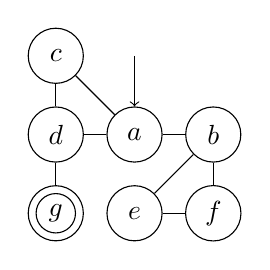
\begin{tikzpicture}[scale=0.5]
    % MDP i
\node [draw, circle, minimum size=0.7cm] (a) at (2, 2) {$a$};
\node [draw, circle, minimum size=0.7cm] (b) at (4, 2) {$b$};
\node [draw, circle, minimum size=0.7cm] (c) at (0, 4) {$c$};
\node [draw, circle, minimum size=0.7cm] (d) at (0, 2) {$d$};
\node [draw, circle, minimum size=0.7cm] (e) at (2, 0) {$e$};
\node [draw, circle, minimum size=0.7cm] (f) at (4, 0) {$f$};
\node [draw, circle, minimum size=0.7cm] (g) at (0, 0) {$g$};
\node [draw, circle, minimum size=0.5cm] at (0, 0) {};

\coordinate[above of=a] (init);

\draw[->] (init) -- (a);
\draw[-] (a) -- (b);
\draw[-] (a) -- (c);
\draw[-] (a) -- (d);
\draw[-] (b) -- (e);
\draw[-] (b) -- (f);
\draw[-] (c) -- (d);
\draw[-] (d) -- (g);
\draw[-] (e) -- (f);
\draw[-] (d) -- (g);

  \end{tikzpicture}
  \caption{状態空間問題の例。エージェントはスタート地点$a$からゴール地点$g$を目指す。
  }
  \label{fig:ssp-graph}
\end{figure}


ユニットコスト状態空間問題はグラフにモデルすることで考えやすくなる。
ユニットコスト状態空間問題を表す\define{状態空間グラフ}{state-space graph}{じょうたいくうかんぐらふ}は以下のように定義される。

\ddef{状態空間グラフ、State-space graph}{
問題グラフ$G = (V, E, s, T)$は状態空間問題$P = (S, A, s, T)$に対して以下のように定義される。ノード集合 $V = S$、初期ノード$s \in S$、ゴールノード集合$T$、エッジ集合$E\subseteq V \times V$。エッジ$u,v\in E$は$a(u) = v$となる$a\in A$が存在する場合に存在し、そしてその場合にのみ存在する(iff)。
}

状態空間問題の\define{解}{solution}{かい}は以下の定義である。

\ddef{解、Solution}{
解$\pi = (a_1,a_2...,a_k)$はアクション$a_i \in A$の(順序付)配列であり、初期状態$s$からゴール状態$t \in T$へ遷移させる。すなわち、$u_i \in S$,$i \in \{0,1,...,k\}$, $u_0 = s, u_k = t$が存在し、$u_i = a_i(u_{i-1})$となる。
}

どのような解を見つけたいかは問題に依存する。
多くの問題では\define{経路コスト}{path cost}{けいろこすと}の合計を小さくすることを目的とする。

%すなわち、アクションに対してコストが定義されており、経路

\ddef{状態空間問題、Weighted state-space problem}{
	状態空間問題$P = (S, A, s, T, w)$はユニットコスト状態空間問題の定義に加え、コスト関数$w: A \rightarrow \mathbb{R}$がある。経路$(a_1,...,a_k)$のコストは$\sum^k_{i=1}w(a_i)$と定義される。
}

%ある解が可能なすべての解の中でコストが最小である場合、その解を最適解(optimal cost solution)であると言う。
本書ではこの状態空間問題を主に扱う。
状態空間問題のうちコストが定数関数である場合がユニットコスト状態空間問題である。
状態空間問題は重み付き(コスト付き)グラフとしてモデルすることが出来る。すなわち、$G = (V, E, s, T, w)$は状態空間グラフの定義に加え、エッジの重み$w: E \rightarrow \mathbb{R}$を持つ。

\ref{ch:blind-search}章で詳解するが、探索アルゴリズムは状態空間グラフのノード・エッジ全てを保持する必要はない。
全てのノード・エッジを保持した状態空間グラフを特に\define{明示的状態空間グラフ}{explicit state-space graph}{めいじてきじょうたいくうかんぐらふ}と呼ぶとする。このようなグラフは、例えば隣接行列を用いて表すことが出来る。隣接行列$M$は行と列の大きさが$|V|$である正方行列であり、エッジ$(v_i, v_j)$が存在するならば$M_{i,j}=1$、なければ$M_{i,j}=0$とする行列である。
このような表現方法の問題点は行列の大きさが$|V|^2$であるため、大きな状態空間を保持することが出来ないことである。
例えば、\ref{sec:search-problem}節で紹介する15-puzzleは状態の数が$|V|=15!/2$であるため、隣接行列を保持することは現在のコンピュータでは非常に困難である。

そこで、探索アルゴリズムは多くの場合初期ノードとノード展開関数による\define{非明示的状態空間グラフ}{implicit state-space graph}{ひめいじてきじょうたいくうかんぐらふ}で表せられる。

\ddef{非明示的状態空間グラフ、Implicit state-space graph}{
	非明示的状態空間グラフ $(s, Goal, Expand, w)$は初期状態$s \in V$、ゴール条件Goal: $V \rightarrow B = \{false, true\}$、ノード展開関数Expand: $V \rightarrow 2^V$、コスト関数$w: V \times V \rightarrow \mathbb{R}$によって与えられる\footnote{$2^V$はノード集合$V$のべき集合である。}。
}

非明示的状態空間グラフも状態空間問題に対して定義できる。明示的状態空間グラフとの違いは次状態の情報が隣接行列ではなくノード展開関数Expandの形に表現されている点である。Expandはある状態からの可能な次の状態の集合を返す関数である。Expand関数は明示的に与えられるのではなく、ルールによって与えられることが多い。例えば将棋であれば、将棋のルールによって定められる合法手によって得られる次の状態の集合がExpand関数によって得られる。多くの場合このノード展開関数は隣接行列よりも小さな情報で表現できる。

本書ではすべてのノードの分枝数が有限であると仮定する (局所有限グラフ、locally finite graph)。% また、コスト関数$w$は非負値であるとする。
また、特に断りがない場合簡単のため$w \geq 0$を仮定する。

% 本書で紹介するアルゴリズムは無限グラフでも完全なものがあるが、局所有限ではないグラフでも完全なものはない。



\section{状態空間問題の例}
\label{sec:search-problem}

状態空間問題の例をいくつか紹介する。
これらの問題はヒューリスティック探索研究でベンチマークとして広く使われているものである。

%グリッド経路探索問題など、応用がありつつ、かつ分かりやすい問題を選んだ。
%グラフ探索アルゴリズムによって効率的に解くことが出来ると知られているドメインをいくつか紹介する。
%ここで詳解する問題はグラフ探索以外の手法でも解くことが出来る。


\subsection{グリッド経路探索 (Grid Path-Finding)}
%\captionlistentry[todo]{Grid Pathfinding: なんかいい感じの絵}
%{\TODO Grid Pathfinding: なんかいい感じの絵}

\define{グリッド経路探索問題}{grid path-finding problem}{グリッドけいろたんさくもんだい}は2次元 (あるいはもっと高次元でもよい) のグリッド上で初期配置からゴール位置までの経路を求める問題である\cite{yap2002grid}。グリッドには障害物がおかれ、通れない箇所がある。エージェントが移動できる方向は4方向($A= \{up, down, left, right\}$)か8方向(4方向に加えて斜め移動)とする場合が多い。自由方向(Any Angle)の問題を扱う研究も存在する\cite{nash2007theta}。

\begin{figure}
        \centering
	% 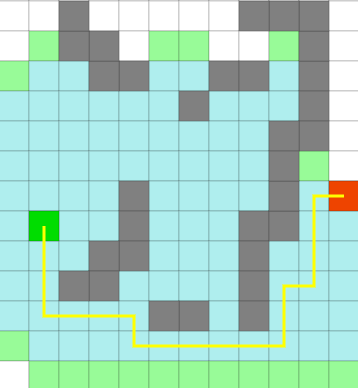
\includegraphics[width=0.5\textwidth]{figures/grid-astar.png}
        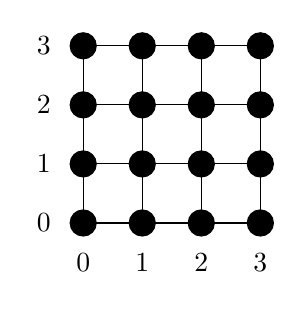
\begin{tikzpicture}[scale=0.5]
          % Grid pathfinding

\foreach \x in {0,...,3}
  \foreach \y in {0,...,3}
    {\node [draw, circle, fill=black] (\x\y) at (1.5*\x, 1.5*\y) {};}

\foreach \x in {0,...,3}
  \foreach \y in {0,...,2}
           {\draw (1.5 * \x, 1.5 * \y) -- (1.5 * \x, 1.5 * \y + 1.5);}

\foreach \y in {0,...,3}
  \foreach \x in {0,...,2}
           {\draw (1.5 * \x, 1.5 * \y) -- (1.5 * \x + 1.5, 1.5 * \y);}
           
\foreach \x in {0,...,3}
         {\node at (1.5 * \x, -1) {\x};
          \node at (-1, 1.5 * \x) {\x};
         }

        \end{tikzpicture}
	\caption{グリッド経路探索問題}
	\label{fig:grid-pathfinding}
\end{figure}


Web上に簡単に試せるデモがあるので、参照されたい\footnote{\url{http://qiao.github.io/PathFinding.js/visual/}}。この本で説明する様々なグラフ探索手法をグリッド経路探索に試すことが出来る。% この本の画像の一部はこのデモをもとに作成している。

グリッド経路探索はロボットのモーションプランニングやゲームAIなどで応用される\cite{algfoor2015comprehensive}。ストラテジーゲームなどでユニット(エージェント)を動かすために使われる \cite{cui2011based,sturtevant2012benchmarks}。% よく使われるベンチマーク問題集にもStarcraftのゲームのマップが含まれている\cite{sturtevant2012benchmarks}.
またグリッドは様々な問題を経路探索に帰着して解くことができるという意味でも重要である。例えば後述する多重整列問題 (Multiple Sequence Alignment)はグリッド経路探索に帰着して解くことが出来る(節 \ref{sec:msa})。
ロボットのモーションプランニングも経路探索問題に帰着することが出来ることがある \cite{barraquand91}。この問題では複数個の関節の角度を変えながら、現在状態から目的の状態 (Configuration)にたどり着けることが目的となる。各関節の角度をグリッドの各次元で表し、ロボットの物理的な構造のために不可能な角度の組み合わせを障害物の置かれたグリッドとすることでグリッド経路探索問題に帰着することができる。このようにモデルを作ると、グリッド上で障害物を避けた経路を計算することで現在状態から目的状態へ関節をうまく動かすモーションプランが発見できる。


\subsection{スライディングタイル (Sliding-tile Puzzle)}

多くの一人ゲームはグラフ探索問題に帰着することが出来る。スライディングタイルはその例であり、ヒューリスティック探索研究においてメジャーなベンチマーク問題でもある (図\ref{fig:15-puzzle}) \cite{johnson1879notes}。
$1$から$(n^2)-1$までの数字が振られたタイルが$n\times n$の正方形に並べられている。正方形には一つだけ{\it ブランク}と呼ばれるタイルのない位置があり、四方に隣り合うタイルのいずれかをその位置に移動する(スライドする)ことが出来る。スライディングタイル問題は、与えられた初期状態からスライドを繰り返し、ゴール状態にたどり着く経路を求める問題である。

\begin{figure}
\centering
% 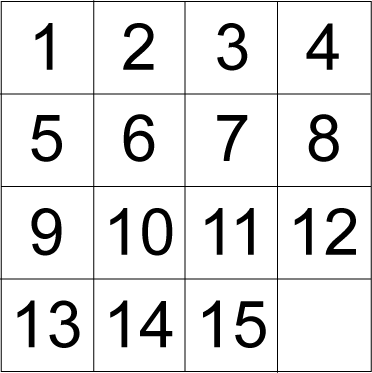
\includegraphics[bb=0 0 372 373,width=0.5\textwidth]{figures/15-puzzle.png}
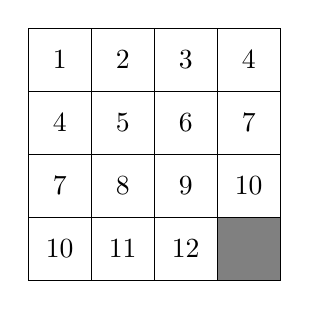
\begin{tikzpicture}[scale=0.8]
  % Sliding tile puzzle

\draw (0, 0) grid (4, 4);

\foreach \x in {0,...,3}
  \foreach \y in {0,...,3}
  {
        \pgfmathsetmacro{\val}{int(\x+3*\y+1)}
        \ifthenelse{\x=3 \AND \y=3}{;}{
          \node at (\x + 0.5, 3 - \y + 0.5) {\val};
        }
  }

\draw[fill=gray] (3,0) rectangle (4, 1);

\end{tikzpicture}
\caption{15パズルのゴール状態の例}
\label{fig:15-puzzle}
\end{figure}


スライディングタイルの到達可能な状態の数は$|V| = (n^2)!/2$\footnote{スライディングタイルは偶奇性があり、到達不可能な状態がある\cite{johnson1879notes}。}であり、$n$に対して指数的に増加する。
可能なアクションは$A= \{up, down, left, right\}$の4つであり、アクションにかかるコストはすべて同じとする。

後述するが、ヒューリスティック探索のためには状態からゴール状態までの距離(コスト)の下界(lower bound)が計算できると有用である。
スライディングタイルにおける下界の求め方として最もシンプルなものは{\it マンハッタン距離ヒューリスティック}である。マンハッタン距離ヒューリスティックは各タイルの現在状態の位置とゴール状態の位置のマンハッタン距離の総和を取る。可能なアクションはすべて一つしかタイルを動かさないので、一回のアクションでマンハッタン距離は最大で1しか縮まらない。よって、マンハッタン距離はゴールまでの距離の下界である。

%ちなみに、スライディングタイルはpermutation problemの一つである。

\subsection{多重整列問題 (Multiple Sequence Alignment)}
\label{sec:msa}
生物学・進化学では遺伝子配列・アミノ酸配列の編集距離(edit distance)を比較することでニ個体がどれだけ親しいかを推定することが広く研究されている。
\define{多重整列問題}{Multiple Sequence Alignment}{たじゅうせいれつもんだい} (MSA)は複数の遺伝子・アミノ酸配列が与えられた時、それらの配列間の編集距離とその時出来上がった配列を求める問題である。
2つの配列に対してそれぞれコストの定義された編集操作を繰り返し、同一の配列に並べ替える手続きをアライメントと呼ぶ。
2つの配列の\define{編集距離}{edit distance}{へんしゅうきょり}は編集操作の合計コストの最小値である。
3つ以上の配列における距離の定義は様々考えられるが、例えば全ての配列のペアの編集距離の総和を用いられる。

MSAにおける可能な編集操作は置換と挿入である。置換は配列のある要素(DNAかアミノ酸)を別の要素に入れ替える操作であり、挿入は配列のある位置に要素を挿入する操作である。例えば(ATG, TGC, AGC)の3つの配列のアライメントを考える。表\ref{tbl:msa-cost}は置換と編集に対するコストの例である。-は欠損を示し、対応する要素が存在しないことを表す。% アミノ酸配列における有名なコスト表としてPAM250\cite{pearson1990}があるが、ここでは簡単のため仮のコスト表を用いる。
表\ref{tbl:msa}はこのコスト表を用いたアライメントの例である。
このとき、例えば配列ATG-と-TGCの編集距離は(A,-)、 (T,T)、 (G,G)、 (-,C)のコストの総和であるので、表\ref{tbl:msa-cost}を参照し、$3+0+0+3=6$である。同様に(ATG-, A-GC)の距離は$9$, (-TGC, A-GC)の距離は$6$であるので、3配列の編集距離は$6+9+6=21$である。

$n$配列のMSAは$n$次元のグリッドの経路探索問題に帰着することが出来る\cite{korf:2000}。
図\ref{tbl:msa-to-grid}は(ATG)と(TGC)の2つの配列によるMSAをグリッド経路探索問題に帰着した例である。
状態$s = (x_1, x_2,...,x_n)$の各変数$x_i$は配列$i$のどの位置までアライメントを完了したかを表す変数であり、配列$i$の長さを$l_i$とすると定義域は$0 \leq x_0 \leq l_0$である。
全てのアライメントが完了した状態$s=(l_1, l_2,...,l_n)$がゴール状態である。
可能なアクション$a=(b_1, b_2, ..., b_n), (b_i=0, 1)$は配列$i$に対してそれぞれ欠損を挿入するか否かであり、配列$i$に対して欠損を挿入する場合に$b_i=0$、挿入しない場合は$b_i=1$となる。
状態$s$に対してアクション$a$を適用した後の状態$s'$は$s'=(x_1+b_1, x_2+b_2,..., x_n+b_n)$となる。図\ref{tbl:msa-to-grid}は初期状態$s=(0,0)$に対して$a=(1,0)$を適用している。これは(A), (-)までアライメントを進めた状態に対応する。次に$a=(1,1)$が適用され、アライメントは(A,T), (-,T)という状態に遷移する。このようにして$(0, 0)$から$(l_1, l_2)$までたどり着くまでの最小コストを求める。

MSAは可能なアクションの数が配列の数$n$に対して指数的に増える ($2^n-1$)点が難しい。アミノ酸配列が対象である場合はコストの値が幅広い点も難しい \cite{pearson1990}。
MSAは生物学研究に役立つというモチベーションから非常に熱心に研究されており、様々な定式化による解法が知られている。
詳しくは\cite{waterman1995introduction,
gusfield1997algorithms,edgar2006multiple}を参照されたい。

\begin{table}
  \centering
  \caption{多重配列問題 (MSA)}
  \begin{tabular}{c|cccc}
    \toprule
	Sequence1 & A & T & G & - \\
	Sequence2 & - & T & G & C \\
	Sequence3 & A & - & G & C \\
        \bottomrule
\end{tabular}
\label{tbl:msa}
\end{table}

\begin{table}
  \centering
\caption{MSAの塩基配列のコスト表}
\begin{tabular}{c|ccccc}
  \toprule
	  & A & T & G & C & - \\ \midrule
	A & 0 & 3 & 3 & 3 & 3 \\
	T & 3 & 0 & 3 & 3 & 3 \\
	G & 3 & 3 & 0 & 3 & 3 \\
	C & 3 & 3 & 3 & 0 & 3 \\
	- & 3 & 3 & 3 & 3 & 0 \\
        \bottomrule
\end{tabular}
\label{tbl:msa-cost}
\end{table}

\begin{table}
  \centering
\caption{MSAのグリッド経路探索問題への帰着}
\begin{tabular}{c|cccc}
  \toprule
	  & A & T & G & - \\ \midrule
	T & $\rightarrow$ & $\searrow$ &   &   \\
	G &   &   & $\searrow$ &   \\
	C &   &   &   & $\downarrow$ \\
        \bottomrule
\end{tabular}
\label{tbl:msa-to-grid}
\end{table}


\subsection{倉庫番 (Sokoban)}
倉庫番(Sokoban)は倉庫の荷物を押していくことで指定された位置に置くというパズルゲームである。現在でも様々なゲームの中で親しまれている \cite{junghanns1997sokoban,culberson:97}。
プレイヤーは「荷物の後ろに回って押す」ことしか出来ず、引っ張ったり、横から動かしたりすることが出来ない。また、荷物の上を通ることも出来ない。
PSPACE-completeであることが知られている\cite{culberson:97}。

%     ####
% #####  #
% #   $  #
% #  .#  #
% ## ## ##
% #      #
% # @#   #
% #  #####
% ####

\begin{figure}
\centering
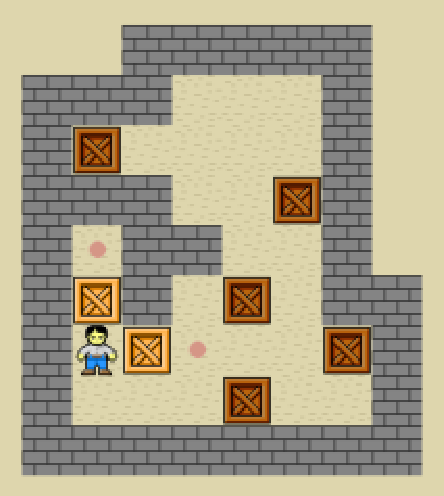
\includegraphics[bb=0 0 213 238,width=0.4\textwidth]{figures/sokoban.pdf}
\caption{倉庫番}
\label{fig:sokoban}
\end{figure}

状態の表現方法は2通りあり、一つはグリッドの各位置に何が置いてあるかを変数とする方法である。もうひとつはプレイヤー、各荷物の位置に対してそれぞれ変数を割り当てる方法である。
可能なアクションは{\tt move-up}, {\tt move-left}, {\tt move-down}, {\tt move-right}, {\tt push-up}, {\tt push-left}, {\tt push-down}, {\tt push-right} の8通りである。{\tt move-*}はプレイヤーが動くアクションに対応し、コストは0である。{\tt push-*}は荷物を押すアクションであり、正のアクションコストが割当てられている。よって、倉庫番はなるべく荷物を押す回数を少なくして荷物を目的の位置に動かすことが目的となる。

グラフ探索問題として倉庫番を考えるときに重要であるのは、倉庫番は\define{不可逆なアクション}{irreversible action}{ふかぎゃくなアクション}が存在することである。
全てのアクション$a \in A$に対して$a^{-1} \in A$が存在し、$a(a^{-1}(s)) = s$かつ$a^{-1}(a(s)) = s$となる場合、問題は\define{可逆}{reversible}{かぎゃく}であると呼ぶ。
例えばグリッド経路探索やスライディングタイルは可逆である。
可逆な問題は対応するアクションのコストが同じであれば無向グラフとしてモデルすることもでき、初期状態から到達できる状態は、すべて初期状態に戻ることが出来る。
一方、不可逆な問題ではこれが保証されず、デッドエンドにはまる可能性がある (\ref{sec:difficulity}節)。

倉庫番では荷物を押すことは出来ても引っ張ることが出来ないため、不可逆な問題である。例えば、荷物を部屋の隅に置いてしまうと戻すことが出来ないため、詰み状態に陥る可能性がある問題である。
このような性質を持つ問題では特にグラフ探索による先読みが効果的である。

倉庫番のもうひとつ重要な性質は\define{ゼロコストアクション}{zero-cost action}{ゼロコストアクション}の存在である。ゼロコストアクションはコストが0のアクションである。%TODO
倉庫番のアクションのうち{\tt move-up}, {\tt move-left}, {\tt move-down}, {\tt move-right}はコストゼロ($w(e)=0$)のアクションである。ヘタなアルゴリズムを実行すると無限に無駄なアクションを繰り返し続けるということもありうるだろう。


\subsection{巡回セールスパーソン問題 (Traveling Salesperson Problem, TSP)}

\begin{figure}
\centering
% 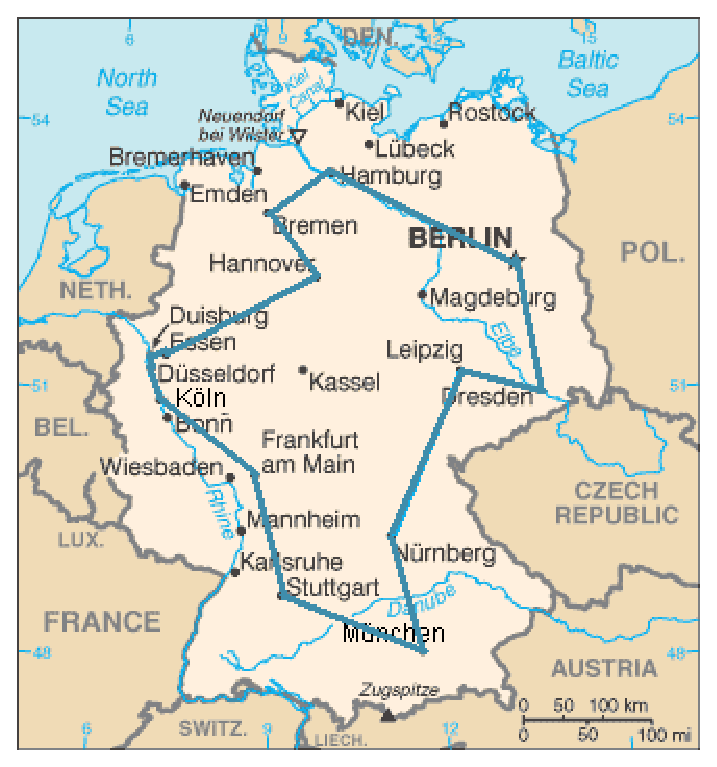
\includegraphics[bb=0 0 328 352,width=0.5\textwidth]{figures/tsp.eps}%TODO 
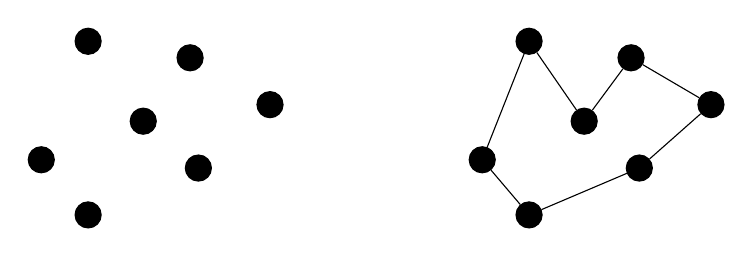
\begin{tikzpicture}[scale=0.7]
  \foreach \x in {0, 8}
  {
    \pgfmathsetmacro{\noise}{0.15}           
\node[draw,circle,fill=black] (1\x) at (\x+0, 0) {};
\node[draw,circle,fill=black] (2\x) at (\x+2, 1-\noise) {};
\node[draw,circle,fill=black] (3\x) at (\x+3+2*\noise, 2) {};
\node[draw,circle,fill=black] (4\x) at (\x+2-\noise, 3-\noise) {};
\node[draw,circle,fill=black] (5\x) at (\x+1, 2-2*\noise) {};
\node[draw,circle,fill=black] (6\x) at (\x+0, 3+\noise) {};
\node[draw,circle,fill=black] (7\x) at (\x-1+\noise, 1) {};
}

\foreach \a in {1,...,6}
  {
    \pgfmathsetmacro{\n}{int(\a+1)}
    \draw[-] (\a8) -- (\n8);
  }

\draw[-] (78) -- (18);

\end{tikzpicture}
\caption{巡回セールスパーソン問題}
\label{fig:tsp}
\end{figure}


巡回セールスパーソン問題は、地図上にある都市を全て回り最初の都市に戻るときの最短距離の経路を求める問題である \cite{applegate2006traveling}。
$n$個の都市があるとすると(非最適解含む)解の数は$(n-1)!/2$個である。
可能なアクションは「都市$i \in \{1..n\}$を訪れる」であり、一度訪れた都市には行けない。
TSPのゴール条件はすべての都市を訪れることである。よって、何も考えずに$n$回アクションを実行すれば、とりあえず解を得ることが出来る。しかし最適解を得ることは難しく、NP完全問題であることが知られている。
TSPはヒューリスティック探索に限らず、様々なアプローチで研究されている実用的に非常に重要なドメインである\cite{applegate2006traveling}。TSPについて特に詳しく知りたい方はそちらの教科書を参照されたい。


\section{問題の性質・難しさ}
\label{sec:difficulity}

本書で定義した状態空間問題は小さなモデルである。
完全情報であり、状態遷移は決定論的である。
% 最小コスト経路探索は
それでもNP困難問題であり、難しい問題は難しい。
この節は問題の難しさがどのような要素に左右されるかを列挙する。

\begin{enumerate}
\item {\bf 状態空間の大きさ}

状態空間の大きさ$|S|$は大きい程概して問題は難しくなる。
特に状態空間が無限である場合深さ優先探索などのアルゴリズムは停止しない場合がある。
例えば状態変数に実数が含まれる場合、状態空間の大きさは無限になる。
% 状態空間の大きさがそのまま問題の難しさに直結するわけではない。

\item {\bf 分枝度}

ある状態$s$の\define{分枝度}{branching factor}{ぶんしど}はそのノードの子ノードの数を指す。
特に状態空間問題の分枝度は、すべての状態の分枝度の平均を指す。ただし多くの場合平均を厳密に求めることはなく、おおよその平均を指して分枝度をすることが多い。
分枝度が大きいほど問題は難しいとは限らない。
分枝度が多いほどグラフが密である、つまりエッジの数が多いことに対応する。
%エッジが多い程解の候補となる経路が多くなる。
分枝度を$b$とすると、あるノード$s$の子ノードの数は$b$個であり、孫ノードの数は$b^2$である。$s$からの深さ$d$のノードは$b^d$個である。

\item {\bf デッドエンド}

問題によってはある状態に到達するともう問題を解くことは出来ないというシチュエーションがある。例えば倉庫番は荷物を角においてしまうともう動かすことができない。これによってもう問題がクリアできなくなるということがある。このような問題では状態空間を広く探索し、デッドエンド状態のみを探索し続けるということをうまく避ける必要がある。例えば\ref{sec:greedy-best-first-search}節の貪欲最良優先探索はデッドエンドに入ってしまうとなかなか抜け出せないかもしれない。
% あるいはデッドエンドを検知する手法も考えられる。
概してデッドエンドがある問題では状態空間を広く探索する手法、探索済みの状態を記録する手法が有利であり、局所探索手法はうまくいかないことがある。
%このような問題では局所探索アルゴリズムではうまくいかないことがある。局所探索アルゴリズムは

\item {\bf 解の存在}

当然解が存在しない問題もありうる。
本書で紹介するアルゴリズムは解が存在しない場合非常に時間がかかるものが多い\footnote{一般にどのようなアルゴリズムを使っても解が存在しない状態空間問題は難しい。}。
一部のアルゴリズムは解が存在しない場合永遠に停止しない場合がある。
そのような場合、アルゴリズムは解が存在しないと示せれば理想的である。
そのため解が存在しないことを検出するアルゴリズムの研究もされている \cite{backstrom2013fast,hoffmann2014distance}。

\end{enumerate}


\section{まとめ}

{\it 状態空間問題}は初期状態とゴール条件が与えられたとき、ゴール条件を満たすための{\it プラン} (行動の列) を見つける問題である。状態空間問題はグラフ上の経路探索問題に帰着できる。このときのグラフを{\it 状態空間グラフ}と呼ぶ。
状態空間グラフを初期ノードとそのノードと隣接するノードを返す{\it ノード展開関数}によって表現することができる。これを{\it 非明示的状態空間グラフ}と呼ぶ。

状態空間問題ではしばしば行動に{\it コスト}が定義されていて、プラン全体の行動コストの総和を最小化することが求められる。
特に全ての行動のコストが同じである場合は{\it ユニットコスト状態空間問題}と呼ぶ。

\section{練習問題}

\begin{enumerate}
  \item ルービックキューブを状態空間問題で表現するとする。このとき、何を状態とするべきか?何を行動とするべきか?
  
  \item スライディングタイル問題でタイルの大きさが$3 \times 3$の時の状態の数はいくつか?$4 \times 4$の時は?
  (ヒント: スライディングタイルには偶奇性があるため、ゴール状態に到達できない盤面がある。)
  
  \item 障害物のない5x5の2次元空間上で上下左右に移動が出来るグリッド経路探索問題を考える。この状態空間における分枝度はいくつか?

  \item (難問) 3x3のスライディングタイル問題における分枝度はいくつかを正確に計算することはできるか?
  
  \item (難問) 状態空間問題として表現することが難しい問題の例を2, 3挙げてみよう。それらの問題を表現するにはどのように状態空間問題を拡張するべきか?
\end{enumerate}


\section{関連文献}

本章で扱うヒューリスティック探索は主にここで定義した状態空間問題への適用を前提として書かれている。
そのため状態空間問題よりも広い問題を解くためには少し工夫が必要になることが多い。

状態空間問題は完全情報であり状態遷移が決定論的であることを仮定した。
状態遷移が決定論的ではなく確率的であると仮定したモデルは\define{マルコフ過程問題}{Markov Decision Process Problem}{マルコフかていもんだい} (MDP)と呼ばれている \cite{puterman2014markov}。
MDP$(S, A, P, R)$は状態集合$S$、アクション集合$A$、状態遷移確率$P$、報酬$R$からなる。
状態空間問題は状態遷移が決定論的であるのに対してMDPのそれは確率的である。
また、MDPはコストを最小化するのではなく報酬の総和の期待値を最大化する問題として定義されることが多い。
状態空間問題はMDPのうち状態遷移が常に決定的であるものである。
MDPは\define{強化学習}{reinforcement learning}{きょうかがくしゅう}における問題モデルとしても広く使われている \cite{sutton:99}。
状態遷移が決定論的であれば、状態遷移は一つの状態から一つの状態へのエッジによって表すことができる。状態遷移が確率的である場合は可能な次状態を列挙するAND-OR木 \cite{luger1997artificial}でモデルすることが出来る。
MDPを解くには動的計画法 \cite{puterman2014markov,barto1995learning}やモンテカルロ木探索 \cite{browne2012survey,kocsis2006bandit}が使われることが多い。

MDPからさらに不完全情報問題に拡張したものを\define{部分観測マルコフ過程問題}{partially observable Markov decision process problem}{ぶぶんかんそくマルコフかていもんだい} (POMDP)と呼ぶ \cite{kaelbling1998planning}。
POMDPにおけるプランニング問題の厳密解はBelief space \cite{kaelbling1998planning}上を探索することで求められるが、多くの場合厳密計算は困難なのでモンテカルロ木探索などの近似手法が用いられる。
POMDPは非常に計算が難しいモデルであるので、仮にPOMDPが与えられた問題をもっとも正確に表せられるモデルであったとしても近似的にMDPを使った方がうまくいくかもしれない。

囲碁やチェスなどの敵対するエージェントがいる問題も探索が活躍するドメインであり、特に二人零和ゲームでの研究が盛んである。
このような問題では敵プレイヤーの取るアクションが事前に分からないのでAND-OR木でモデルすることが多い。
敵対ゲームを解くための手法としてはMiniMax木、$\alpha$-$\beta$木\cite{pearl84}やモンテカルロ木探索などがある。近年では強化学習によってヒューリスティック関数を学習するアプローチが盛んに研究されている \cite{sutton:99}。

ヒューリスティック探索はゲームやロボティクスの応用の中で現れる経路探索問題を解くために特によく使われる。
ゲームに探索を使う場合問題になるのは計算にかかる時間である。
たとえば次の一手を計算するために一日以上かかるチェスAIとプレイしたい人は少ないだろう。
このような応用では解のコストだけでなく、解を得るために使う時間も評価しなければならない。
このような問題をリアルタイム探索と呼ぶ \cite{korf90,barto1995learning}。
リアルタイム探索にはLearning real-time A* (LRTA*) \cite{korf90,koenig2001minimax}やReal-time adaptive A* (RTAA*) \cite{koenig2006real}などが使われる。

本書ではノードの次数が有限 (局所有限グラフ)である問題を対象としたアルゴリズムを紹介している。
一見自然な仮定だが、この仮定ではアクションや状態空間の大きさが無限である連続空間問題を解くことができない。そのためロボティクスで現れる連続空間問題を解くためには工夫が必要になる。
例えばグリッド経路探索問題で任意の角度を取ることが出来るAny-angle path planning問題は本書では扱わないが、ヒューリスティック探索の派生アルゴリズムで解くことができる\cite{lavalle2006planning,lavalle2001rapidly,daniel2010theta,nash2013any}。

状態空間問題は制約充足問題の一種であり、Boolean satisfiability problem (SAT)として書くことができる \cite{garey1979computers}。それを利用してSATによって状態空間問題を解くアプローチも広く研究されている \cite{kautz1992planning,kautz2006satplan,rintanen2012planning}。状態空間問題では表現することが難しい制約や目的関数がある場合は制約充足問題や離散最適化問題としてモデルすることもできる。


% -*- coding: utf-8 -*-
%%%%%%%%%%%%%%%%%%%%%%%%%%%%%%%%%%%%%%%%%%%%%%%%%
%%% CHAPTER: Blind Search
%%%%%%%%%%%%%%%%%%%%%%%%%%%%%%%%%%%%%%%%%%%%%%%%%
\chapter{情報なし探索 (Blind Search)}
\label{ch:blind-search}

\ref{ch:introduction}章では様々な状態空間問題を紹介したが、それぞれの問題の解法はどれも沢山研究されている。
一つの指針としては、ある問題に特化した解法を研究することでその問題をより高速に解くというモチベーションがある。
これは例えばMSAのように重要なアプリケーションがある問題の場合に特に熱心に研究されることが多い。
一方、なるべく広い範囲の問題に対して適用可能な手法を研究するというモチベーションもある。
{\bf この章で紹介する手法は問題特化のアルゴリズムよりもパフォーマンスに劣るが、問題の知識をあまり必要とせず、さまざまな問題に適用できる}。
%ただしこのような手法はドメインに特化したプログラムと比べてパフォーマンスに劣ることが多い。

\ref{ch:introduction}章で紹介した状態空間問題を広く扱うことの出来る手法としてグラフ探索アルゴリズムがある。
本章では最もシンプルな問題(ドメイン)の知識を利用しない探索を紹介する。
情報なし探索 (Blind Search)は状態空間グラフのみに注目し、背景にある問題に関する知識を一切使わないアルゴリズムである。
このような探索では{\bf 1. 重複検知を行うか 2. ノードの展開順序}が重要になる。
重複検出は訪問済みの状態を保存しておくことで同じ状態を繰り返し探索することを防ぐ手法である。対価としては、メモリの消費量が非常に大きくなることにある。
ノードの展開順序とは、例えば幅優先探索・深さ優先探索などのバリエーションを指す。
効率的な展開順序は問題によって大きく異なり、問題を選べばこれらの手法によって十分に効率的な探索を行うことが出来る。
これらの探索手法は競技プログラミングでもよく解法として使われる\cite{skiena2006programming}。また、いわゆるコーディング面接でもグラフ探索アルゴリズムは頻出である\cite{mcdowell2011cracking}。
%\ref{ch:search-performance}章はグラフ探索の高速化の紹介をするので、特に競技プログラミングに興味がある場合はそちらも参照されたい。% TODO
情報なし探索は\cite{cormen01}の22章Elementary Graph Algorithmsにも詳しく説明されている。


\section{木探索アルゴリズム (Tree Search Algorithm)}
\label{sec:tree-search-algorithm}
木探索アルゴリズムはグラフ探索アルゴリズムの基礎となるフレームワークであり、本文で紹介する手法のほとんどがこのフレームワークを基礎としているといえる。
アルゴリズム\ref{alg:implicit-tree-search}は木探索の疑似コードである。

\begin{algorithm}[h]
\caption{木探索 (Implicit Tree Search)}
\label{alg:implicit-tree-search}
	\Input{非明示的状態空間グラフ $(s, Goal, Expand, w)$, プライオリティ関数 $f$}
	\Output{$s$からゴール状態への経路、経路が存在しなければ$\emptyset$}
	$Open \leftarrow \{s\}$, $d(s) \leftarrow 0$, $g(s) \leftarrow 0$\;
	\While{$Open \neq \emptyset$} {
                $u \leftarrow \argmin_{u' \in Open} f(u')$ \;
		$Open \leftarrow Open \setminus \{u\} $\;
		\If {$Goal(u)$} {
			\Return $Path(u)$\;
		}
		\For {each $v \in Expand(u)$} {
 			$Open \leftarrow Open \cup \{u\}$\;
		        $d(v) \leftarrow d(u) + 1$\;
		        $g(v) \leftarrow g(u) + w(u, v)$\;
			$parent(v) \leftarrow u$\;
		}
 	}
	\Return $\emptyset$\;
\end{algorithm}
    
木探索はオープンリスト\footnote{歴史的な経緯でリストと呼ばれているが、データ構造がリストで実装されるという意味ではない。効率的なデータ構造は\ref{ch:search-performance}章で紹介する。}と呼ばれるノードの集合をPriority queueに保持する。探索の開始時には、初期状態のみがオープンリストに入っている。
木探索は、このオープンリストから一つノード$u$を選び、ゴール条件を満たしているかを確認する。満たしていれば初期状態から$u$への経路を返す。満たしていなければ、そのノードを展開する。展開とは、そのノードの子ノードを列挙し、オープンリストに入れることを指す。

\begin{figure}
  \centering
  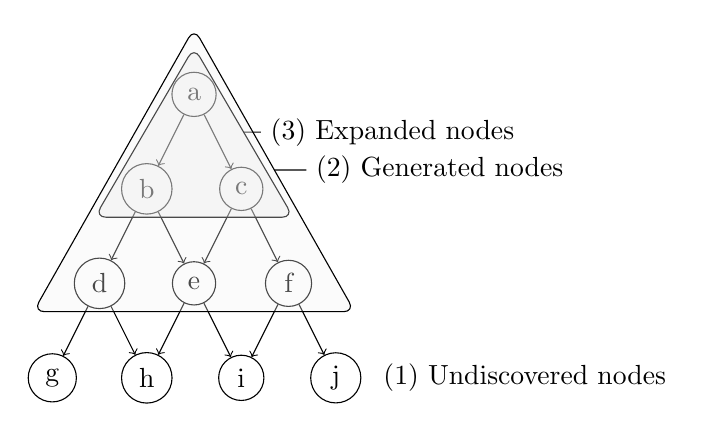
\begin{tikzpicture}[scale=0.6]
    % Reexpansion

\node [draw,circle] (a) at ( 0, 4) {a};

\node [draw,circle] (b) at (-1, 2) {b};
\node [draw,circle] (c) at ( 1, 2) {c};

\node [draw,circle] (d) at (-2, 0) {d};
\node [draw,circle] (e) at ( 0, 0) {e};
\node [draw,circle] (f) at ( 2, 0) {f};

\node [draw,circle] (g) at (-3,-2) {g};
\node [draw,circle] (h) at (-1,-2) {h};
\node [draw,circle] (i) at ( 1,-2) {i};
\node [draw,circle] (j) at ( 3,-2) {j};

\draw[->] (a) -- (b);
\draw[->] (a) -- (c);

\draw[->] (b) -- (d);
\draw[->] (b) -- (e);
\draw[->] (c) -- (e);
\draw[->] (c) -- (f);

\draw[->] (d) -- (g);
\draw[->] (d) -- (h);
\draw[->] (e) -- (h);
\draw[->] (e) -- (i);
\draw[->] (f) -- (i);
\draw[->] (f) -- (j);



% expanded nodes
\draw[rounded corners, fill=gray!20, fill opacity=0.3] (0, 4 + 1) -- (-1 - 1.1, 2 - 0.6) -- (1 + 1.1, 2 - 0.6) -- cycle;

\node (label3) at (4.2, {((4+1) + (2 - 0.6)) / 2}) {(3) Expanded nodes};

\coordinate (draw3) at ({(0 + (1 + 1.1)) / 2}, {((4+1) + (2 - 0.6)) / 2});
\draw[-] (draw3) -- (label3);

% generated nodes
\draw[rounded corners, fill=gray!10, fill opacity=0.3] (0, 4 + 1 + 0.4) -- (-2 - 1.4, 0 - 0.6) -- (2 + 1.4, 0 - 0.6) -- cycle;

\node (label2) at (5.2, {((4+1+0.4) + (0 - 0.6)) / 2}) {(2) Generated nodes};

\coordinate (draw2) at ({(0 + (2 + 1.4)) / 2}, {((4+1+0.4) + (0 - 0.6)) / 2});
\draw[-] (draw2) -- (label2);


\node at (7, -2) {(1) Undiscovered nodes};


  \end{tikzpicture}
  \caption{未生成・生成済み・展開済みノードの例。木探索は生成済みノードのうち展開済みでないものをひとつ取り出し、そのノードを展開し子ノードを得る。新しく得られた子ノードは未生成ノードから生成済みノードとなり、展開したノードは展開済みノードになる。}
  \label{fig:node-life}
\end{figure}

各ノードの注目すると、ノードは1. 未生成、2. 生成済み、3. 展開済みと状態が遷移していく。

\begin{enumerate}
\item 未生成ノード (Undiscovered nodes): 状態空間内のまだ生成されていないノード。非明示的グラフでは情報は保持されていない。
\item 生成済みノード (Generated nodes): オープンリストに一度でも入れられたノード。後述するグラフ探索ではクローズドリストに入れられる。
\item 展開済みノード (Expanded nodes): $Expand$を実行し終えたノード。子ノードがすべて生成済みノードになる。オープンリストからは取り除かれる。
\end{enumerate}

図\ref{fig:node-life}は探索アルゴリズムが$\{a, b, c\}$を展開し終えた時点でのノードの分類の例である。
$\{a, b, c\}$は展開済みノードであり、同時に生成済みノードである。これらのノードは後述するグラフ探索ではクローズドリストと呼ばれるデータ構造に入れられ、保持される。これらのノードの子ノードがすべて生成される。$\{d, e, f\}$は生成済みノードであるが展開済みではない。探索アルゴリズムのオープンリストにはこれらのノードが入っている。$\{g, h, i, j\}$は未生成のノードであり、アルゴリズムからは見えない未発見のノードである。
例えば次に$d$を展開すると、展開済みノードは$\{a, b, c, d\}$となり、新たに$\{g, h\}$が未生成ノードから生成済みノードに遷移する。このように探索が進行していくことによってノードは順次状態遷移していく。


初期状態からノード$n$への最小ステップ数を深さ$d$と呼び、最小経路コストを$g$値と呼ぶ。すべてのアクションのコストが1のドメインであれば任意の$n$に対して$d(n) = g(n)$が成り立つ。
状態を更新すると同時に$g$値を更新する。これによって解を発見した時に解ノードの$g$値が解のコストとなる。
なお、状態$s$に対して適用可能なアクションの集合$A(s)$は与えられていると仮定する。

$Path(u)$はノードに対して初期状態からそこへ到達するまでの経路を返す関数である。$(u, parent(u), parent(parent(u)),...,s)$のように再帰的に$parent$を初期状態まで辿る。

{\bf 紛らわしいが、木探索アルゴリズムは木だけでなくグラフ一般を探索するアルゴリズムである。}
木探索の強みは生成済みノードのうち展開済みではないもののみをオープンリストに保持すればよいことにある。未生成ノード、展開済みノードはメモリ上に保持する必要がない。
一方これの問題は、一度展開したノードが再びExpandによって現れた場合\define{再展開}{reexpansion}{さいてんかい}をすることになる。図\ref{fig:reexpansion}の例ではノード$d$に二通りの経路で到達できるが、木探索では二回目に$d$に到達したとき、すでに到達済みであることを把握できない。そのため同じノードを再び生成・展開することになる。
このように木探索は複数の経路で到達可能なノードがあるほど(グラフがより木から遠いほど)同じノードを何度も再展開することになり、効率が悪くなってしまう。

また、木探索アルゴリズムは状態数が有限であっても停止しない場合がある。
これらが問題になるような問題ドメインである場合は後述する重複検出を使うグラフ探索 (\ref{sec:graph-search-algorithm}節)を使うと良いだろう。


\begin{figure}
  \centering
  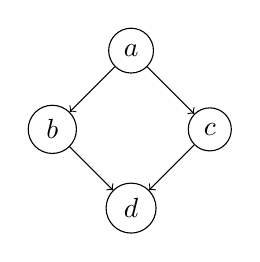
\begin{tikzpicture}[scale=0.5]
    % Reexpansion

\node [draw,circle] (a) at ( 0, 4) {$a$};
\node [draw,circle] (b) at (-2, 2) {$b$};
\node [draw,circle] (c) at ( 2, 2) {$c$};
\node [draw,circle] (d) at ( 0, 0) {$d$};

\draw[->] (a) -- (b);
\draw[->] (b) -- (d);

\draw[->] (a) -- (c);
\draw[->] (c) -- (d);

  \end{tikzpicture}
  \caption{ノードの再展開の例}
  \label{fig:reexpansion}
\end{figure}


オープンリストはプライオリティキューであり、どの順番でノードを取り出すかを決めなければならない。プライオリティ$f$の選択は探索アルゴリズムの性能に強く関係する。
本章の\ref{sec:breadth-first-search}節以降、及び\ref{ch:heuristic-search}章はこのプライオリティをどうデザインするかについて議論をする。

%木探索ベースのアルゴリズムの問題は、解が存在しない場合に停止性を満たさないことである。よって、この手法は解が間違いなく存在することが分かっている問題に対して適用される。あるいは、解が存在することを判定してから用いる。


\section{グラフ探索アルゴリズム (Graph Search Algorithm)}
\label{sec:graph-search-algorithm}


明示的グラフのあるノードが初期状態から複数の経路でたどり着ける場合、同じ状態を表すノードが木探索による非明示的グラフに複数現れるということが生じる。このようなノードを\define{重複}{duplicate}{ちょうふく}と呼ぶ。ノードの重複は計算資源を消費してしまうので、効率的な\define{重複検出}{duplicate detection}{ちょうふくけんしゅつ}の方法は重要な研究分野である。
{\bf 本書ではノードの重複検出を行う探索アルゴリズムを狭義にグラフ探索アルゴリズムと呼び、重複検出を行わない探索を狭義に木探索アルゴリズムと呼ぶ。}


\begin{algorithm}[tbh]
\caption{グラフ探索 (Implicit Graph Search)}
\label{alg:implicit-graph-search}
	\Input{非明示的状態空間グラフ $(s, Goal, Expand, w)$、プライオリティ関数 $f$}
	\Output{$s$からゴール状態への経路、経路が存在しなければ$\emptyset$}
	$Open \leftarrow \{s\}$, $Closed \leftarrow \{s\}$, $d(s) \leftarrow 0$, $g(s) \leftarrow 0$\;
	\While{$Open \neq \emptyset$} {
                $u \leftarrow \argmin_{u' \in Open} f(u')$ \;
		$Open \leftarrow Open \setminus \{u\} $\;
		\If {$Goal(u)$} {
			\Return $Path(u)$\;
		}
		\For {each $v \in Expand(u)$} {
		  \If{$v \notin Closed$ {\bf or} $g(u) + w(u, v) < g(v)$} {
                    $Open \leftarrow Open \cup \{v\}$\;
		    $d(v) \leftarrow d(u) + 1$\;
		    $g(v) \leftarrow g(u) + w(u, v)$\;
                    $parent(v) \leftarrow u$\;
                  }
		  \If{$v \notin Closed$} {
                    $Closed \leftarrow Closed \cup \{v\}$\;
                  }
		}
 	}
	\Return $\emptyset$\;
\end{algorithm}


重複検出のためには生成されたノードを\define{クローズドリスト}{closed list}{クローズドリスト}に保存する。一度クローズドリストに入れられたノードはずっとクローズドリストに保持される。
ノード展開関数から子ノードが生成されたら、その子ノードと同じ状態を保持するノードがクローズドリストに存在するかを確認する。
もし存在しなければ、そのノードは重複ではない。なのでそのノードをオープンリストに加える。
存在した場合の処理は少しややこしい。
新たに生成されたノード$n$の$g$値のほうが先に生成されクローズドリストにあるノード$n'$の$g$値よりも小さい場合が存在する。このとき、$n$をそのまま捨ててしまうと、そのノードの$g$値が本来の値よりも大きく評価されてしまう。

$g$値をそのノードに到達できる既知の最小コストにするためには、まずクローズドリストに保存されているノードの$g$値を$g(n')$から$g(n)$に更新しなければならない。
加えて、ノード$n$を\define{再展開}{reexpansion}{さいてんかい}しなければならない。
ノード$n$の子ノード$c$は$n'$の子ノードとして展開されていたわけであるが、そのとき$g(c) = g(n') + w(n', c)$として計算された。この値は$g(c) = g(n) + w(n, c)$に更新しなければならない。$w(n', c) = w(n, c)$なので、$g(n') - g(n)$だけ$g$値が小さくなる。なので、$c$の子ノードも再展開をする必要がある。そしてそのまた子ノードも。。。というように、再展開が生じるとそこから先のノードをすべて再展開する必要がある。これはかなり大きなコストになることが多いので、可能な限り避けたい処理である。

%なので常に$g$値をそのノードに到達できる既知の最小コストに更新する。

重複が存在した場合に必ずノードを捨てることができる場合も存在する。
まず、解の最適性が必要でない場合$g$値を更新する必要はない。$g$値が過大に評価されても解経路は解経路のままであり、ただ解経路のコストが大きくなるだけである。
また、例えば幅優先探索では探索の過程で生成されるノードの$d$値は単調増加する。もしユニットコストドメインならば$g$値も単調増加である。つまりノード$n$と重複したノード$n'$がクローズドリストにあったとすると、$g(n) \geq g(n')$が成立する。この場合、解最適性を保ったまま$n$を安全に捨てることができる。
また、状態空間グラフが木である場合は重複が発生しない。
なお、後述するA*探索\ref{sec:astar-search}ではある条件を満たせば再展開は行わずに解の最適性が満たせることが知られている。これがA*探索がstate-of-the-artとして重要視されている理由である。

ここで「ノード」と「状態」の言葉の使い分けに注意したい。
状態とは状態空間問題における状態$s$である。ノードは状態$s$を含み、$f$値、$g$値の情報を含む。
重複検出を行わない木探索の場合、同じ状態を保持するノードが2つ以上存在しうる。
重複検知は同じ状態を保持するノードをマージする処理に相当する。この処理を行うと同じノードに複数の経路で到達するようになり、グラフは木ではなくなる。

% 重複検出を行ってもノードの再展開が必要になる場合は存在するが、ほとんどの場合重複検出を行わない場合よりもはるかに再展開の回数は少なくなる。
% 実行時間で見ると重複検出を行ったほうがほぼ確実に効率的である。
重複検出の問題はメモリの使用量である。重複検出を行うためには生成済みノードをすべてクローズドリストに保存しなければならない。なので展開済みノードの数に比例した空間が必要になる。
クローズドリストの効率的な実装については\ref{sec:closed-list}節で議論をする。

なお、重複検出はノードが生成されたときではなく、ノードが展開されるときに遅らせることができる。
オープンリストには重複したノードが含まれることになるが、ノードの展開時には重複をチェックするので重複したノードの展開は防げる、ということである。これは\define{遅延重複検出}{delayed duplicate detection}{ちえんちょうふくけんしゅつ}と呼ばれ、\ref{sec:delayed-duplicate-detection}節で議論をする。



\section{幅優先探索 (Breadth-First Search)}
\label{sec:breadth-first-search}

探索のパフォーマンスにおいて重要になるのは{\bf どのようにして次に展開するノードを選択するか}にある。
ヒューリスティック探索の研究の非常に大きな部分はここに費やされているといえる。
シンプルかつ強力なノード選択方法はFirst-in-first-out (FIFO)である。あるいは幅優先探索と呼ぶ。

幅優先探索の手順は非常に単純であり、FIFOの順に$Open$から取り出せばいいだけである。
これをもう少し大きな視点で、{\it どのようなノードを優先して探索しているのか}を考えてみたい。
初期状態から現在状態にたどり着くまでの経路の長さをノードの$d$値と定義する。
すると、幅優先探索のプライオリティ関数$f$は$d$値と一致する。

\begin{equation}
  f_{\text{brfs}}(s) = d(s)
\label{alg:brfs-open}
\end{equation}

ユニットコスト問題である場合、更に$g$値とも一致する ($f_{\text{brfs}}(s) = d(s) = g(s)$)。

幅優先探索のメリットは最初に発見した解が最短経路長の解であることである。
問題がユニットコストドメインであれば、最短経路が最小コスト経路であるので、最適解が得られる。
なお、後述するBest First Searchと区別するため、Breadth-First Searchの略称はBrFSを用いることがある (Best First SearchはBFSとなる)。

重複検出を用いた幅優先探索で図\ref{fig:ssp-graph}の問題を解こうとすると、オープンリスト、クローズドリストの中身は表\ref{tbl:brfs-traj}のように遷移する。
図\ref{fig:ssp-tree}の探索木を見比べながら確認してみてほしい。

\begin{figure}
  \centering
  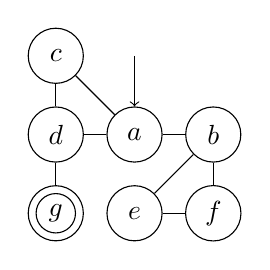
\begin{tikzpicture}[scale=0.5]
    % MDP i
\node [draw, circle, minimum size=0.7cm] (a) at (2, 2) {$a$};
\node [draw, circle, minimum size=0.7cm] (b) at (4, 2) {$b$};
\node [draw, circle, minimum size=0.7cm] (c) at (0, 4) {$c$};
\node [draw, circle, minimum size=0.7cm] (d) at (0, 2) {$d$};
\node [draw, circle, minimum size=0.7cm] (e) at (2, 0) {$e$};
\node [draw, circle, minimum size=0.7cm] (f) at (4, 0) {$f$};
\node [draw, circle, minimum size=0.7cm] (g) at (0, 0) {$g$};
\node [draw, circle, minimum size=0.5cm] at (0, 0) {};

\coordinate[above of=a] (init);

\draw[->] (init) -- (a);
\draw[-] (a) -- (b);
\draw[-] (a) -- (c);
\draw[-] (a) -- (d);
\draw[-] (b) -- (e);
\draw[-] (b) -- (f);
\draw[-] (c) -- (d);
\draw[-] (d) -- (g);
\draw[-] (e) -- (f);
\draw[-] (d) -- (g);

  \end{tikzpicture} \hspace{20pt}
  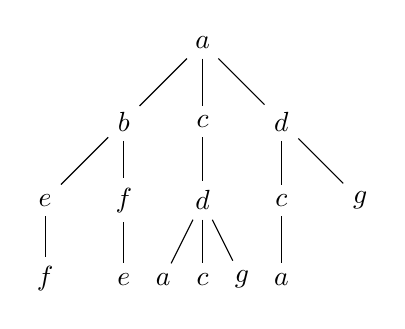
\begin{tikzpicture}[scale=0.5]
    % MDP i
\node (a0) at (4, 6) {$a$};

\node (b1) at (2, 4) {$b$};
\node (c1) at (4, 4) {$c$};
\node (d1) at (6, 4) {$d$};

\node (e2) at (0, 2) {$e$};
\node (f2) at (2, 2) {$f$};
\node (d2) at (4, 2) {$d$};
\node (c2) at (6, 2) {$c$};
\node (g2) at (8, 2) {$g$};

\node (f3) at (0, 0) {$f$};
\node (e3) at (2, 0) {$e$};
\node (a31) at (3, 0) {$a$};
\node (c3) at (4, 0) {$c$};
\node (g3) at (5, 0) {$g$};
\node (a32) at (6, 0) {$a$};

\draw[-] (a0) -- (b1);
\draw[-] (a0) -- (c1);
\draw[-] (a0) -- (d1);
\draw[-] (b1) -- (e2);
\draw[-] (b1) -- (f2);
\draw[-] (c1) -- (d2);
\draw[-] (d1) -- (g2);
\draw[-] (d1) -- (c2);
\draw[-] (e2) -- (f3);
\draw[-] (f2) -- (e3);
\draw[-] (d2) -- (a31);
\draw[-] (d2) -- (c3);
\draw[-] (d2) -- (g3);
\draw[-] (c2) -- (a32);

  \end{tikzpicture}
  \caption{探索木}
  \label{fig:ssp-tree}
\end{figure}


\begin{table}[tbh]
\centering
\caption{重複検出を用いた幅優先グラフ探索のオープンリスト・クローズドリスト (\cite{edelkamp:2010:hst:1875144}より)}
\begin{tabular}{c|c|l|l|l}
  \toprule
	ステップ & ノードの選択 & オープンリスト & クローズドリスト & コメント \\ \midrule
	1 	  & \{\}       & \{a\}      & \{\} \\
	2     & a        & \{b,c,d\}  & \{a\} \\
	3     & b        & \{c,d,e,f\} & \{a,b\} \\
	4     & c        & \{d,e,f\}   & \{a,b,c\} \\
	5     & d        & \{e,f,g\}   & \{a,b,c,d\} \\
	6     & e        & \{f,g\}     & \{a,b,c,d,e\} \\
	7     & f        & \{g\}       & \{a,b,c,d,e,f\} \\
	8     & g        & \{\}        & \{a,b,c,d,e,f,g\} & ゴール \\
        \bottomrule
\end{tabular}
\label{tbl:brfs-traj}
\end{table}

\section{深さ優先探索 (Depth-First Search)}
\label{sec:depth-first-search}

幅優先探索が幅を優先するのに対して深さ優先探索はもっとも深いノードを優先して探索する。

\begin{equation}
  f_{\text{dfs}}(s) = -d(s)
\label{alg:dfs-open}
\end{equation}

深さ優先探索は解がある一定の深さにあることが既知である場合に有効である。
例えばTSPは全ての街を回ったときのみが解であるので、街の数が$n$であれば全ての解の経路長が$n$である。
このような問題を幅優先探索で解こうとすると、解は最も深いところにしかないので、最後の最後まで解が一つも得られないということになる。一方、深さ優先探索なら$n$回目の展開で一つ目の解を見つけることが出来る。
表\ref{tbl:dfs-traj}は図\ref{fig:ssp-graph}の問題で重複検出ありの深さ優先探索を行った場合のオープンリスト・クローズドリストの遷移を示した。図\ref{fig:ssp-tree}と合わせてノードが展開される順序を確認すると良い。

深さ優先探索は無限グラフにおいて、解が存在しても永遠に停止しない場合がある。幅優先探索であれば解がある場合、いずれそれを発見する (解の深さを$d^*$とすると、$d(s) \leq d^*$であるノードの数は有限であるので)。しかし深さ優先探索は停止しない場合がある。

良い解、最適解を見つけたい場合でも深さ優先探索が有用である場合がある。
早めに一つ解が見つけられると、その解よりも質が悪い解にしかつながらないノードを\define{枝刈り}{pruning}{えだがり}することが出来る。ノード$n$を枝刈りするとは、ノード$n$をオープンリストに加えずそのまま捨てることを指す。つまりアルゴリズム\ref{alg:implicit-tree-search}における$Open \leftarrow Open \cup \{v\}$をスキップする。このような枝刈りを用いた探索アルゴリズムを\define{分枝限定法}{Branch-and-Bound}{ぶんしげんていほう}と呼ぶ。

\begin{table}[tbh]
\centering
\caption{重複検出を用いた深さ優先グラフ探索のオープンリスト・クローズドリスト (\cite{edelkamp:2010:hst:1875144}より)}
\begin{tabular}{c|c|l|l|l}
  \toprule
	ステップ & ノードの選択 & オープンリスト   & クローズドリスト & コメント \\ \midrule
	1 	  & \{\}     & \{a\}       & \{\} \\
	2     & a        & \{b,c,d\}   & \{a\} \\
	3     & b        & \{e,f,c,d\} & \{a,b\} \\
	4     & e        & \{f,c,d\}   & \{a,b,e\} \\
	5     & f        & \{c,d\}     & \{a,b,e,f\} \\
	6     & c        & \{d\}       & \{a,b,e,f,c\} \\
	7     & d        & \{g\}       & \{a,b,e,f,c,d\} \\
	8     & g        & \{\}        & \{a,b,e,f,c,d,g\} & ゴール \\
        \bottomrule
\end{tabular}
\label{tbl:dfs-traj}
\end{table}

\subsection{再帰による深さ優先探索}
\label{sec:recursive-depth-first-search}

上述の実装はオープンリストを利用した深さ優先探索である。
アルゴリズム \ref{alg:implicit-tree-search}を元にした深さ優先探索の実装は効率的ではないことが多い。
深さ優先探索は再帰によって効率的に実装することができる (アルゴリズム \ref{alg:recursive-dfs})。
再帰実装ではオープンリストがないことに注目したい。
再帰を利用することでデータ構造を明に保存する必要がなくなり、キャッシュ効率が良くなることがある。
幅優先探索も同様に再帰によって実装することが出来るが、効率的であるケースはあまりない。

\begin{algorithm}[tbh]
\caption{DFS: 再帰による深さ優先探索 (Depth-First Search)}
\label{alg:recursive-dfs}
	\Input{非明示的状態空間グラフ $(s, Goal, Expand, w)$、前状態 $s'$}
	\Output{$s$からゴール状態への経路、経路が存在しなければ$\emptyset$}
	\If {$Goal(s)$} {
		\Return $s$\;
	}
	\For {each $u \in Expand(s) \setminus \{s'\}$} {
          $v \leftarrow DFS(u, Goal, Expand, w, s)$\;
	  \If {$v \neq \emptyset$} {
	    \Return $(s, DFS(v, Goal, Expand, w, u))$
	  }
	}
	\Return $\emptyset$\;
\end{algorithm}


\section{ダイクストラ法 (Dijkstra Algorithm)}
\label{sec:dijkstra}

\define{ダイクストラ法}{Dijkstra's Algorithm}{ダイクストラほう}はグラフ探索アルゴリズムの一種であり、グラフ理論の教科書な
どでも登場する情報科学全体に多岐に渡り重要とされるアルゴリズムである \cite{dijkstra1959note}。
例えばネットワークルーティングにおけるlink state algorithmなどにDijkstraが使われる\cite{mcquillan1980new}。
%初期状態からノード$n$への既知の最小経路コストを$g$値と呼び、$g(n)$と書く。
ダイクストラ法はグラフ探索において$g$値が最も小さいノードを優先して展開するアルゴリズムと説明することができる。

\begin{equation}
  f_{\text{bfs}}(s) = g(n)
\end{equation}

{\bf ダイクストラ法は重複検出を行うグラフ探索アルゴリズムである。}
ダイクストラ法は非負コストグラフにおいて最短経路を返す。
ユニットコストドメインでは$\forall n (g(n) = d(n))$であるため、幅優先探索と同じ動作をする。
フィボナッチヒープを用いてオープンリストを実装したダイクストラ法は$O(|E| + |V|log|V|)$時間でであることが知られている\cite{fredman1987fibonacci}。
そのため、後述するヒューリスティック関数が得られない問題においてはとりあえずダイクストラ法を試してみることは有効である。


\section{情報なし探索の比較}
\label{sec:blind-comparison}

探索アルゴリズムの評価指標としては以下の四点が重要である。

\begin{enumerate}
\item 完全性: 解が存在するとき、有限時間内に解を返すか。
\item 最適性: 最初に発見された解が最適解か。
\item 時間: アルゴリズムの実行にかかる時間
\item 空間: アルゴリズムの実行にかかる空間
\end{enumerate}

完全なアルゴリズムであることは有用だが、時間・空間とのトレードオフにあることが多い。
完全であっても実現可能な時間・空間で実行することが出来なければ意味がないので、完全でない高速なアルゴリズムを選択する方が良い場合もある。
最適性も同様に時間・空間とのトレードオフにあることが多いので、解きたい問題に最適な解が必要かどうかを考える必要がある。
また、後述するwA* (節\ref{sec:weighted-astar-search})は発見された解が最適解のコスト$c^*$の定数倍以下であることを保証する近似アルゴリズムである。


表\ref{tbl:comparison}は情報なし探索をこれら四点で比較している。
反復深化深さ優先は節\ref{sec:depth-first-iterative-deepening}、両方向探索は節\ref{sec:bidirectional-search}で紹介する。
$b$は分枝数、$d$は解の深さ、$m$は可能な探索木の深さの最大値である。
重複検出を行うグラフ探索の場合、深さ優先探索は有限グラフならば完全であり、時間・空間は状態空間の大きさ$|S|$でバウンドされる。
この表にある時間・空間量は理論的な最悪の場合の比較である。解きたい問題にかかる平均的な性能は必ずしもこれに相関しない。最終的には実験的なベンチマークを行い良いアルゴリズムを選択する必要がある。

\begin{table}[tbh]
\centering
\caption{木探索アルゴリズムの比較 (\cite{russelln03}のFigure 3.21より)}
\resizebox{\textwidth}{!}{
\begin{tabular}{c|cccc}
  \toprule
  性能  & 幅優先探索 & 深さ優先探索 & 反復深化深さ優先 & 両方向幅優先探索 \\ \midrule
  完全性 & 局所有限グラフならYes & No & 局所有限グラフならYes & 局所有限グラフならYes \\
  最適性 & ユニットコストならYes & No & ユニットコストならYes & ユニットコストならYes \\
  時間  & $O(b^d)$ & $O(b^m)$ & $O(b^d)$ & $O(b^{d/2})$ \\
  空間  & $O(b^d)$ & $O(bm)$  & $O(bd)$ & $O(b^{d/2})$ \\
  \bottomrule
\end{tabular}
}
\label{tbl:comparison}
\end{table}


\section{まとめ}

状態空間問題を解くための手法としてグラフ探索アルゴリズムがある。グラフ探索アルゴリズムは1. 展開するノードの順序と2. 展開したノードの処理の2点で特徴づけることが出来る。
{\it 幅優先探索}は{\it オープンリスト}の中から深さが浅いノードから優先して探索し、{\it 深さ優先探索}は逆に深いノードから優先して探索する。{\it ダイクストラ法}はコストが小さいノードから優先して探索するため、最短経路を最初に見つけることができる。
木探索は展開したノードを保持せず同じ状態を複数回重複して展開してしまうリスクがある。グラフ探索は展開済みノードを{\it クローズドリスト}に保存しておくことで重複展開を防ぐ。一方メモリ消費量が大きくなるというデメリットがある。

探索アルゴリズムの選択において考慮するべきことは主に以下の4点である。解が存在するとき、有限時間内に解を返すか ({\it 完全性})、最初に発見された解が最適解か (最適性)、アルゴリズムの実行にかかる時間と空間。



\section{練習問題}


1. 幅優先木探索を実装し、$3 \times 3$のスライディングタイルを解いてみよう。

2. 重複検出を使った幅優先探索を実装し、$3 \times 3$のスライディングタイルを解いてみよう。重複検出を使わない幅優先木探索と比べて展開したノードの数は?重複検出によって枝刈りされたノードの数は?

3. 重複検出を使った深さ優先探索を実装し、$3 \times 3$のスライディングタイルを解いてみよう。見つけた解は1, 2で見つけた解と比べて長いか?

4. 重複検出を使った幅優先探索で巡回セールスパーソン問題を解いてみよう。この時、見つかった解は最短経路だったか?

5. ダイクストラ法を実装し、巡回セールスパーソン問題を解いてみよう。この時、見つかった解は最短経路だったか?


\section{関連文献}

時間・空間制約が厳しい場合は反復深化探索、両方向探索や並列探索を使えば解決できることがある。
これらのアルゴリズムについては\ref{ch:heuristic-search-variants}章で紹介する。

ダイクストラ法はコストが負のエッジを持つ場合にうまくいかない。
負のエッジを含む問題を解くための手法としてはベルマン-フォード法が有名である \cite{bellman1958routing,ford1956network}。

No Free Lunch定理\cite{wolpert1997no}はコンピュータサイエンスの多くの最適化問題で言及される定理である。
状態空間問題におけるNo Free Lunch定理の主張はざっくりと説明すると以下である。
\dtheorem{
すべての可能なコスト関数による状態空間問題のインスタンスの集合を考える。
この問題集合に対する平均性能はすべての探索アルゴリズムで同じである。
}
つまり、問題の知識が何もなければ「効率的なアルゴリズム」というものは存在しない。
問題に対して知っている知識を利用することによってはじめて探索を効率的にすることができる。
すなわち、状態空間問題のインスタンスの一部分で性能を犠牲にすることで、他のインスタンス集合への性能を向上させることができる。例えば解の長さが20以下であるという知識があるとすれば、探索を深さ20までで打ち切ると良いと考えられる。この探索アルゴリズムは解の長さが20以下であるインスタンスに対しての性能は良くなるが、解の長さが20より大きいインスタンスの性能は著しく悪くなる。このように知識を利用して探索の方向性を変えることがグラフ探索では重要になる。
それが次章で扱うヒューリスティック探索の肝である。




% -*- coding: utf-8 -*-
%%%%%%%%%%%%%%%%%%%%%%%%%%%%%%%%%%%%%%%%%%%%%%%%
%%%%%%%%%%%%%%%%%%%%%%%%%%%%%%%%%%%%%%%%%%%%%%%%
%%%%%%%%%%%%%%%%%%%%%%%%%%%%%%%%%%%%%%%%%%%%%%%%
\chapter{ヒューリスティック探索 (Heuristic Search)}
\label{ch:heuristic-search}

\ref{ch:blind-search}章では問題の知識を利用しないグラフ探索手法について解説した。
本章では問題の知識を利用することでより効率的なグラフ探索を行う手法、特にヒューリスティック探索について解説する。

\section{ヒューリスティックとは?}
\label{sec:heursitic}

\begin{figure}
  \centering
  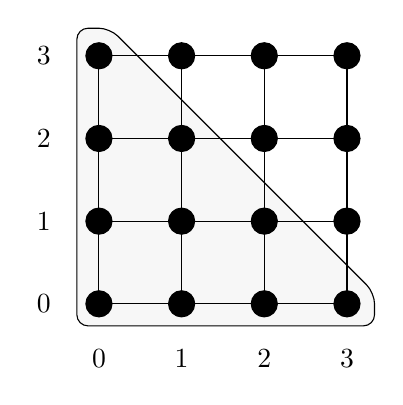
\begin{tikzpicture}[scale=0.7]
    % BrFS region

\draw[rounded corners, fill=gray!20, fill opacity=0.3] (-0.4, -0.4) -- (3*1.5+0.5, -0.4) -- (3*1.5+0.5, 0.2) -- (0.2, 3*1.5+0.5) -- (-0.4, 3*1.5+0.5) -- cycle;


% Grid pathfinding

\foreach \x in {0,...,3}
  \foreach \y in {0,...,3}
    {\node [draw, circle, fill=black] (\x\y) at (1.5*\x, 1.5*\y) {};}

\foreach \x in {0,...,3}
  \foreach \y in {0,...,2}
           {\draw (1.5 * \x, 1.5 * \y) -- (1.5 * \x, 1.5 * \y + 1.5);}

\foreach \y in {0,...,3}
  \foreach \x in {0,...,2}
           {\draw (1.5 * \x, 1.5 * \y) -- (1.5 * \x + 1.5, 1.5 * \y);}
           
\foreach \x in {0,...,3}
         {\node at (1.5 * \x, -1) {\x};
          \node at (-1, 1.5 * \x) {\x};
         }

  \end{tikzpicture}
  \caption{グリッド経路探索におけるダイクストラ法}
\label{fig:grid-brfs}  
\end{figure}

経路探索問題をダイクストラ法で解くことを考えよう。
図\ref{fig:grid-brfs}のグリッド経路探索問題で(0, 0)の位置から(3, 0)の位置まで移動するため経路を求める問題を考えよう。
このときダイクストラ法が探索していく範囲は図\ref{fig:grid-brfs}の灰色のエリアにあるノードになる。
しかし人間が経路探索を行うときにこんなに広い領域を探索しないだろう。グリッドの右側、ゴールのある方向に向かってのみ探索するだろう。なぜか。
それは人間が問題の特徴を利用して、このノードを展開したほうがよいだろう、このノードは展開しなくてよいだろう、という直感を働かせているからである。
問題の特徴を利用してノードの{\bf 有望さ}を\define{ヒューリスティック関数}{heuristic function}{ヒューリスティックかんすう}として定量化し、それを探索に利用したアルゴリズムを\define{ヒューリスティック探索}{heuristic search}{ヒューリスティックたんさく}と呼ぶ。
% ヒューリスティック関数は人間が自分の知識を利用してコーディングする場合と、自動的に生成する場合もある。

% \begin{figure}
% \centering
% \subfloat[幅優先探索]{
% \includegraphics[width=0.45\textwidth]{figures/grid-brfs.png}
% \label{fig:grid-dijkstra}
% } \hspace{4pt}
% \subfloat[ヒューリスティック探索]{
% \includegraphics[width=0.45\textwidth]{figures/grid-astar-mdheuristic.png}
% \label{fig:grid-astar-mdheuristic}
% }
% \end{figure}


\section{ヒューリスティック関数 (Heuristic Function)}
\label{sec:heuristic-function}
ヒューリスティック関数は状態の有望さの評価値であり、多くの場合その状態からゴールまでの最短距離の見積もりであることが多い \cite{hart68formal}。

\ddef{ヒューリスティック関数、heuristic function}{
	ヒューリスティック関数$h$はノードの評価関数である。$h: V \rightarrow \mathbb{R}_{\geq 0}$
}
ヒューリスティックの値が小さいノードほどゴールに近いと推測できるので、探索ではヒューリスティック値が小さいノードを優先して展開する。
ヒューリスティック関数の値をそのノードの$h$値と呼ぶ。

ヒューリスティック関数の望ましい性質として、まず正確である方が望ましい。すなわち、$h$値が実際のゴールまでの最短距離に近いほど、有用な情報であると言える。
ノード$u$からゴールまでの正しい最短コストを$h^*(u)$とする。
ヒューリスティック関数$h$が任意のノード$u$に対して$h(u) = h^*(u)$である場合、\define{完璧なヒューリスティック}{Perfect Heuristic}{かんぺきなヒューリスティック}と呼ぶ。完璧なヒューリスティックがある場合、ほとんどの場合その問題を一瞬で解くことができる。現実には完璧なヒューリスティックはなかなか得られないが、ヒューリスティック関数がこれに近いほど必要な展開ノード数が小さいことが多い\cite{helmert:08}。
%完璧なヒューリスティック関数がある場合、A*探索は
反対に役に立たないヒューリスティック関数は$\forall u \in V: h(u) = 0$などの定数関数である。これはどのノードに対してもゴールまでの距離が同じだと推測しているということであり、つまり何も主張をしていない。定数関数をヒューリスティックに使った探索を\define{ブラインド探索}{blind search}{ブラインドたんさく}と呼ぶ。\ref{ch:blind-search}章で扱った情報なし探索はヒューリスティック探索の特別な場合と考えることができる。


もう一つ望ましい性質は$h$値が最適解コストの下界である場合である。
\ref{sec:astar-search}章で解説するが、$h$値が最短距離の下界である場合、それを用いた効率的な探索アルゴリズム(A*探索、重み付きA*探索)において解コストに理論的保証が得られることが広く知られている。
$h$値が常に最適解コストの下界であるヒューリスティック関数を\define{許容的なヒューリスティック}{admissible heuristic}{きょようてきなヒューリスティック}と呼ぶ。

\ddef{許容的なヒューリスティック、admissible heuristic}{
	ヒューリスティック関数$h$は最適解のコストの下界である場合、許容的である。すなわち、全てのノード$u \in V$に対して$h(u) \leq h^*(u)$が成り立つ。
}

ただし、$h^*(u)$はノード$u$からゴールノード集合$T$のいずれかへたどり着くための最短経路である。%$h^*$はパーフェクトヒューリスティックと呼ぶ。

一般に、許容的なヒューリスティックを得る方法としては、元問題の\define{緩和問題}{relaxed problem}{かんわもんだい}を解き、その最適解コストをヒューリスティック値とすることである。ある問題の緩和問題とは、解集合に元の問題の解を含む問題を指す。要するに元の問題より簡単な問題である\footnote{解が多いほど簡単であるとは一概には言えないが}。

%許容的よりも強い性質としてとして無矛盾性がある。

もう一つ有用なヒューリスティックは\define{無矛盾なヒューリスティック}{consistent heuristic}{むむじゅんなヒューリスティック}である。

\ddef{無矛盾なヒューリスティック、consistent heuristic}{
	ヒューリスティック関数$h$は全てのノードのペア$(u, v)$に対して
        \begin{equation}
                h(u) \leq h(v) + k(u,v)
        \end{equation}
        が成り立つ場合、無矛盾である。$k(u, v)$は$u$から$v$へ至るための最小コストである (経路がない場合$k = \infty$とする)。
}

無矛盾性は特に\ref{sec:astar-search}章で後述するA*探索において探索の効率性に重要な性質である。
また、無矛盾なヒューリスティックのうちゴールノードの$h$値が0となるヒューリスティックは許容的である。

\dtheorem{
ゴールノード$t \in T$に対して$h(t) = 0$となる無矛盾なヒューリスティックは許容的なヒューリスティックである。
}

\begin{proof}
        $t \in T$とする。
        すべてのノード$u \in V$に対して以下が成り立つ。
\begin{align}
	h(u) &\leq h(t) + k(u, t) \\
             &= k(u, t) \\
             &= h^*(u)
\end{align}
        よって$h(u) \leq h^*(u)$より許容的である。
\end{proof}

ゴールノードに対してヒューリスティック値が$0$になるヒューリスティック関数を作ることは簡単である。単純に$Goal(u)$ならば$h(u)=0$とすればよい。
ヒューリスティックの無矛盾性は証明することは難しそうであるが、実はシンプルな導き方がある。そのためにまず\define{単調なヒューリスティック}{monotone heuristic}{たんちょうなヒューリスティック}を定義する。

\ddef{単調なヒューリスティック、monotone heuristic}{
	ヒューリスティック関数$h$は全てのエッジ$e = (u, v) \in E$に対して$h(u) \leq h(v) + w(u,v)$が成り立つ場合、無矛盾である。
}

単調なヒューリスティックは無矛盾性の定義と比較して、ノードのペア$(u, v)$が直接繋がっているという制約がある分、弱い性質に思えるかもしれない。しかし実は単調性と無矛盾性は同値である。


\dtheorem{
        単調性と無矛盾性は同値である。
}
\dproof{
        無矛盾性であるならば単調性であることは自明である。
        単調性が成り立つ場合に無矛盾であることを示す。
        $(u, v)$に経路がない場合$k=\infty$なので
\begin{align}
	h(u_0) &\leq h(u_1) + w(u_0, u_1) \\
			&\leq h(u_2) + w(u_0, u_1) + w(u_1, u_2) \\
			&... \\
			&\leq h(u_k) + \sum_{i=0..k-1}(w(u_i,u_{i+1})) \\
\end{align}
        $u = u_0, v = u_k$とすると無矛盾性が成り立つ。
}

よって、無矛盾性を示すために必要なのは直接つながっているノードのペアに対して$h(u) \leq h(v) + w(u,v)$が成り立つことを示せばよい。これを示すことは比較的にシンプルである。

これらのアルゴリズムの性質は後述するA*探索において非常に有用である。
%無矛盾性の主張は、ヒューリスティックの値が小さいほどゴールに近いということを意味する。つまり、ノード$n_0, n_1$に対して$h(n_0) < h(n_1)$ならば、$n_0$からゴールへの最小コストは$n_1$からゴールへの最小コストよりも小さい。
%これのうれしい点は、次にどのアクションを選択するべきかを考える際、よりゴールに近いノードに向かったほうが良いだろう、と判断をすることができる点にある。
%例えばグリッド経路探索問題におけるマンハッタン距離ヒューリスティックは無矛盾なヒューリスティックである。マンハッタン距離ヒューリスティックは現在位置とゴール位置のマンハッタン距離を$h$値とする。


\section{A*探索 (A* Search)}
\label{sec:astar-search}

\begin{figure}
  \centering
  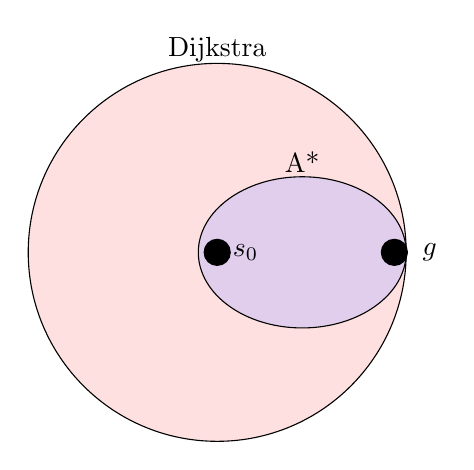
\begin{tikzpicture}[scale=0.6]
    % BrFS region

\pgfmathsetmacro{\x}{2}

\draw[fill=red!30, fill opacity=0.4] (0, 0) circle (2*\x);
\draw[fill=blue!30, fill opacity=0.4] ({0.9*\x}, 0) ellipse ({1.1*\x} and {0.8*\x});

\node[draw,circle,fill=black] (a) at (0,0) {};
\node (aa) at (0+0.6, 0) {$s_0$};

\node[draw,circle,fill=black] (b) at (2*\x-0.25,0) {};
\node (bb) at (2*\x+0.5,0) {$g$};


\node (d) at (0, 2*\x+0.3) {Dijkstra};
\node (a) at ({0.9*\x}, {0.8*\x+0.3}) {A*};

  \end{tikzpicture}
  \caption{A* (ヒューリスティック探索)とダイクストラ法 (情報なし探索)の探索範囲の比較}
\label{fig:dijkstra-astar}  
\end{figure}

ダイクストラ法は初期状態からそのノードまでのコストである$g$値が最小のノードを展開していく。これは間違った方針ではないだろうが、理想的にはゴール状態に向かっていくノードを展開していきたい。図\ref{fig:dijkstra-astar}の大きい方の円はダイクストラ法 (情報なし探索)による状態空間の探索を図示したものである。ダイクストラ法はゴールがどこにあるかということを無視して探索を進めているため、初期位置からどの方向へも均等に探索を行う。
人間の目で見れば一目で右に探索していけばよいというのは分かる。そのような人間の持っている知識を利用して探索を効率化出来ないだろうか?
\define{A*探索}{A* search}{エースターたんさく}はゴールまでの距離を見積もる\define{ヒューリスティック関数}{heuristic function}{ヒューリスティックかんすう}を用いることでゴールに向かって探索していくことを目指した手法である。

A*探索はヒューリスティック探索の代名詞である、最も広く知られている手法である \cite{fikes:71}。
A*探索は以下の$f$値が最小となるノードを優先したグラフ探索アルゴリズムである。

\begin{equation}
  f_{\text{A*}}(u) = g(u) + h(u)
\label{alg:astar-search}
\end{equation}

\begin{figure}
  \centering
  \begin{tikzpicture}[scale=0.6]
    % BrFS region

\pgfmathsetmacro{\x}{3}

\node[draw,circle,fill=black] (s0) at (0,0) {};
\node (ss) at (0, 0 - 0.6) {$u_0$};

\node[draw,circle,fill=black] (t) at (2*\x,0) {};
\node (gg) at (2*\x,0 - 0.6) {$t$};


\node[draw,circle,fill=black] (c) at (\x * 0.8, 0.5 * \x) {};
\node (cc) at (\x * 0.8, 0.5 * \x - 0.6) {$u$};


\draw[->] (s0) -- (c) node[above,pos=0.5] {$g(u)$};
\draw[->,dashed] (c) -- (g) node[above,pos=0.5] {$h(u)$};


  \end{tikzpicture}
  \caption{$f_{\text{A*}}$値の意味}
  \label{fig:fvalue}
\end{figure}


ノード$u$の$f$値は、初期状態$u_0$から$u$を通過してゴール状態$t \in T$に辿り着くためのコストの見積もりである (図 \ref{fig:fvalue})。$g$値は初期状態からノード$u$までの既知の最短経路コストである。一方$h$値はヒューリスティック関数による$u$からゴール状態までの最短経路の見積もりである。
A*探索は非明示的グラフ探索アルゴリズム(アルゴリズム\ref{alg:implicit-graph-search})の一つであり、$f$値が最小ノードから優先して探索を行う \ref{alg:astar-search}。

% $g(n)$のみでノードを選択するダイクストラ法(\ref{sec:dijkstra}章)と比較すると、A*探索はゴール状態までのコストの見積もりを考慮して次に展開するノードを決めている。

% 図\ref{fig:grid-astar-mdheuristic}は\define{マンハッタン距離ヒューリスティック}{Manhattan distance heuristic}{マンハッタンきょりヒューリスティック}によるA*探索である。
% 青いノードは展開済みノード、緑のノードはオープンリストに入れられた未展開ノードである。幅優先探索による図\ref{fig:grid-dijkstra}と比較すると、展開済み・未展開ノードの数が少なく済んでいることがわかるだろう。


\dtheorem{
  グラフに経路コストが0以下のサイクルが存在しない場合、A*は完全である。  
}
\dproof{
  グラフが有限である場合は、やがてすべてのノードを生成・展開し解を発見するので、完全である。
  グラフが無限である場合もやがて解を発見できる。最適解のコストを$c^*$とすると、A*が展開するノードは$f(u) \leq c^*$のノードのみである。本書ではグラフは局所有限であると仮定している (すべてのノードの分枝数は有限である)ので、$f(u) \leq c^*$を満たすノードは有限個である。A*探索はやがてこれらのノードをすべて生成・展開し解を発見するので、完全である。
}
なお、解が存在しない場合、グラフが無限である場合にA*は停止しないので停止性を満たさない。


A*に用いるヒューリスティック関数は正確であるほど良いが、それに加えて許容的、無矛盾であるという性質も有用である。

\dtheorem{
ヒューリスティックが許容的である時、A*は最適解を返す。
}
\dproof{

%全てのノードnは展開時にg(n)がnに辿り着くための最短経路コストの値である。%これは無矛盾性か
許容的なヒューリスティック$h(u)$は$u$からゴールへの経路の下界である。よって、ゴール状態の$h$値は$0$である。つまりゴール状態の$f$値は$g$値と同じである。この解の$g(v)$値を$f^*$と置く(解のコストに相当)。
A*のノードの展開順に従うと、$f^*$のノードを展開する前に全ての$f<f^*$のノードが展開される。
これらのノードがいずれもゴール状態でなければ、$g(u) \leq f(u)$より、$g(u)<f^*$となるゴール状態がない。すなわち、$f^*$が最適解のコストとなり、$v$がその時のゴール状態である。

}

A*探索はノードの\define{再展開}{reexpansion}{さいてんかい}が生じる可能性がある。
アルゴリズム\ref{alg:implicit-graph-search}にあるように、すでに訪れた状態に再び訪れたとき、前に訪れたときよりも小さな$g$値で訪れた場合、ノードを再展開する。このとき、その状態から先の部分木もより小さな$g$値で訪れることになるので、部分木をすべて更新しなければならない。そのため、ノードの再展開によってかなり性能が落ちてしまうことがある。
無矛盾なヒューリスティックの魅力はA*で再展開が生じないことにある。

\dtheorem{
無矛盾なヒューリスティックを用いたA*探索はノードの再展開が生じない。
}

無矛盾なヒューリスティックである場合、A*探索は全てのノード$u \in S$に最初に最短経路コストで訪れることが証明できる。そのため再展開が生じない。

効率的なA*探索のためには良いヒューリスティック関数をデザインしたい。
許容的で無矛盾なヒューリスティックであると解析的に良い性質を満たしていると言える。
一方、経験的に速いと知られているヒューリスティック関数の中にはこれらの性質を満たしていないものも多い。


A*に用いるヒューリスティック関数は正確であるほどより探索範囲を狭めることができる。

\ddef{ヒューリスティックの情報} {
  ヒューリスティック$h_1$とヒューリスティック$h_2$が両方許容的であり、かつすべてのゴールでない$u \in V \setminus T$に対して
  \begin{equation}
    h_2(u) > h_1(u)
  \end{equation}
  であるとき、$h_2$は$h_1$よりも\define{情報がある}{more informed}{ヒューリスティックの情報}と呼ぶ。
}

より情報があるヒューリスティックを使う方がA*は効率的である。

\dtheorem{
  (ノード展開の必要条件): A*探索で展開されるノードの$f$値はすべて最適解のコスト以下である ($f(u) \leq c^*$)。
}

\dtheorem{
  (ノード展開の十分条件): $f$値が最適解のコスト未満であるノードは必ずすべてA*探索で展開される ($f(u) < c^*$)。
}

A*探索は$f$値が一番小さいノードから展開していくので、これらの定理が満たされる。

\dtheorem{
  $h_2$が$h_1$よりも情報がある場合、$h_2$を使ったA*探索によって展開されるノードはすべて$h_1$を使ったA*探索でも展開される。
}
\dproof{
  $h_2$によるA*で展開されるノードの集合はすべて$c^* \geq g(u) + h_2(u)$である。
  ゴールを除き$g(u) + h_2(u) > g(u) + h_1(u)$である。
  よって、$c^* > g(u) + h_1(u)$なのでこれらのノードはすべて$h_1$を使ったA*探索でも展開される。
} 

よって、A*に使うヒューリスティックは情報があるほど良い。


一方のヒューリスティック関数が他方より情報がある場合はより情報のある方を使えばよい。
しかし、ある場所では$h_1$よりも$h_2$の方が正確であり、他のある場所では$h_2$よりも$h_1$の方が正確である、となる場合がある。この場合どちらのヒューリスティックを使えば良いだろうか?実は両方を使うことによってより良い正確なヒューリスティックを得ることができる。

\dtheorem{
  \begin{itemize}
    ヒューリスティック$h_1,..., h_m$が許容的であるとき、$h(u) = \max(h_1(u),..., h_m(u))$は許容的である。
    ヒューリスティック$h_1,..., h_m$が許容的で無矛盾であるとき、$h(u) = \max(h_1(u),..., h_m(u))$は許容的で無矛盾である。
  \end{itemize}
}

このように複数のヒューリスティックを組み合わせることでより良いヒューリスティックを得ることができる。
このアイディアはさまざまなヒューリスティック関数の自動生成に応用されている。


\section{ヒューリスティック関数の例}
\label{sec:heuristic-example}

\ref{sec:heuristic-function}章にあるように、なるべく正確であり、許容的、無矛盾なヒューリスティックが望ましい。
一般に、許容的なヒューリスティックを得る方法としては、元問題の{\bf 緩和問題}を解き、その最適解コストをヒューリスティック値とすることである。ある問題の緩和問題とは、解集合に元の問題の解を含む問題を指す。要するに元の問題より簡単な問題である\footnote{解が多いほど簡単であるとは一概には言えないが}。
グラフ探索アルゴリズムにおいて緩和問題を作る方法は様々あるが、一つはグラフのエッジを増やすことで緩和が出来る。グラフのエッジを増やすには、問題の可能なアクションを増やすなどの方法がある。

\subsection{グリッド経路探索:マンハッタン距離}

4方向グリッド経路探索問題の元問題は障害物のあるグリッドに移動することは出来ない。グリッド経路探索で有効なヒューリスティックの一つはマンハッタン距離ヒューリスティックである。これは現在位置とゴール位置のマンハッタン距離を$h$値とする。マンハッタン距離は障害物を無視した (全ての隣り合うグリッド間にエッジが存在すると仮定した)最短経路の距離である (図\ref{fig:md})ので、元の問題グラフに対してグラフのエッジを増やした緩和問題での解のコストに対応する。
このように、問題の性質を理解していれば許容的なヒューリスティック関数を設計することが出来る。

\begin{figure}
  \centering
  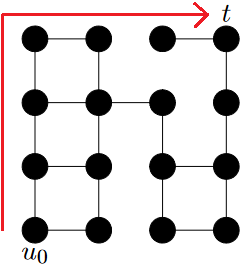
\includegraphics{figures/manhattan-distance.png}
\caption{グリッド経路探索におけるマンハッタン距離。図の赤線は障害物を無視した最短経路である。その距離は必ず実際の最短経路の長さ以下になる。}
\label{fig:md}
\end{figure}


\subsection{スライディングタイル:マンハッタン距離}
スライディングタイルにおけるマンハッタン距離ヒューリスティックは各タイルの現在の位置とゴール状態の位置のマンハッタン距離の総和を$h$値とする。
タイルの現在の位置とゴール状態の位置のマンハッタン距離は、実際にそのタイルが動く距離以下になる。
また、スライディングタイル問題において一つのアクションで動かせるタイルは1つである。
よって$h$は実際に各タイルが動く距離の総和以下であるので、マンハッタン距離ヒューリスティックは許容的なヒューリスティックである。

\subsection{スライディングタイル:パターンデータベース}

\define{パターンデータベースヒューリスティック}{Pattern database heuristic}{パターンデータベースヒューリスティック}は部分問題を解き、その解コストをヒューリスティック値とするアルゴリズムである\cite{edelkamp2001planning}。
探索を始める前に部分問題を解き、部分問題のすべての状態からゴール状態への最適解のコストをテーブルに保存する。
図\ref{fig:pattern-database}はスライディングタイルにおけるパターンデータベースの例である。
図の例は「1, 2, 3, 4のタイルを正しい位置に動かす」という部分問題を解いている。
この部分問題では5, 6, 7, 8のタイルの位置はどこでもよい。1, 2, 3, 4さえゴール位置にあればよい。
ゴール条件以外は元の問題と同様である。
この部分問題は元の問題の緩和問題になっているので許容的なヒューリスティックが得られる。

図の例では1, 2, 3, 4のタイルに絞った部分問題だったが、他のタイルの組み合わせでも良い。
例えば1, 2, 3, 4のタイルによる部分問題と5, 6, 7, 8のタイルによる部分問題からは異なるヒューリスティック値を得ることができる。
これらのヒューリスティック値の最大値を取ることでより正確なヒューリスティックにすることができる。
このように複数のパターンデータベースを使うヒューリスティックを\define{複数パターンデータベース}{multiple pattern databse}{ふくすうパターンデータベース}と呼ぶ \cite{holte:04}。複数パターンデータベースは一つの大きなパターンデータベースを使うよりも正確さに欠けるが、計算時間・空間の面で大きなアドバンテージがある。

1, 2, 3, 4のタイルによる部分問題と5, 6, 7, 8のタイルによる部分問題は一見完全に分割された部分問題なので、これらのヒューリスティック値の和を取ってもよさそうだが、そうすると許容的なヒューリスティックにはならない。なぜなら例えばタイル5を動かすアクションによるコストは両方の部分問題のコストに数えられているからである。
そこで部分問題のコストを「1, 2, 3, 4 (あるいは5, 6, 7, 8)のタイルを動かすときのみコストがかかり、他のタイルはコスト0で動かせる」とすると、コストを重複して数えることはなくなる。そうするとこれらの部分問題のコストの和は許容的なヒューリスティックになる。
このように複数のパターンデータベースで重複してコストが数えられないようにしたものを\define{素集合パターンデータベース}{disjoint pattern databse}{そしゅうごうパターンデータベース}と呼ぶ \cite{korf2002,felner2004additive,yang2008general}。 % TODO: good term?

マンハッタン距離ヒューリスティックは、各タイルごとの部分問題8つに分けた場合の素集合パターンデータベースであると考えることができる。
素集合パターンデータベースは複数のデータベースに分けることでデータベース構築にかかる計算コストが減少するが、その代わりヒューリスティック関数の精度が悪くなる。

\begin{figure}
  \centering
  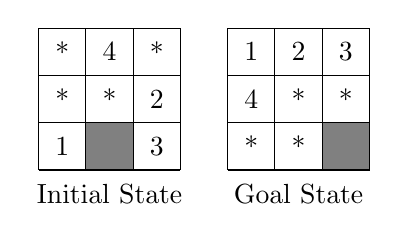
\begin{tikzpicture}[scale=0.6]
    
%%% Initial state

\draw (0, 0) grid (3, 3);


\node at (0 + 0.5, 0 + 0.5) {1};
\draw[fill=gray] (1,0) rectangle (2, 1);
\node at (2 + 0.5, 0 + 0.5) {3};

\node at (0 + 0.5, 1 + 0.5) {*};
\node at (1 + 0.5, 1 + 0.5) {*};
\node at (2 + 0.5, 1 + 0.5) {2};

\node at (0 + 0.5, 2 + 0.5) {*};
\node at (1 + 0.5, 2 + 0.5) {4};
\node at (2 + 0.5, 2 + 0.5) {*};

\node at (1.5, -0.5) {Initial State};

%%% Goal state
\pgfmathsetmacro{\base}{4}

\draw (\base+0, 0) grid (\base+3, 3);

\foreach \x in {0,...,2}
{
  \foreach \y in {0,...,2}
  {
        \pgfmathsetmacro{\val}{int(\x+3*\y+1)}
        \ifthenelse{\x=2 \AND \y=2}{;}{
          \ifthenelse{\val>4}{
            \node at (\base+\x + 0.5, 2 - \y + 0.5) {*};
          }{
            \node at (\base+\x + 0.5, 2 - \y + 0.5) {\val};
          }
        }
  }
}
\draw[fill=gray] (\base+2,0) rectangle (\base+3, 1);

\node at (\base+1.5, -0.5) {Goal State};

  \end{tikzpicture}
\caption{パターンデータベースの初期状態 (左)とゴール条件 (右)の例。1, 2, 3, 4のタイルだけゴール位置にあればよく、他のタイルの位置は関係ない。}
\label{fig:pattern-database}
\end{figure}


\subsection{巡回セールスパーソン問題:最小全域木}
TSPの解の下界としては\define{最小全域木}{minimum spanning tree}{さいしょうぜんいきき}のコストがよく用いられる (図\ref{fig:tsp-mst})。
グラフの\define{全域木}{spanning tree}{ぜんいきき}は全てのノードを含むループを含まない部分グラフである。
最小全域木は全域木のうち最もエッジコストの総和が小さいものである。
未訪問の都市によるグラフの最小全域木はTSPの下界となることが知られている。
まだ訪問していない都市をカバーする最小全域木のコストをヒューリスティック関数に用いることができる。
最小全域木はヒューリスティックの精度は良くはないが素早く計算ができるメリットがある。

\begin{figure}[tbh]
  \centering
  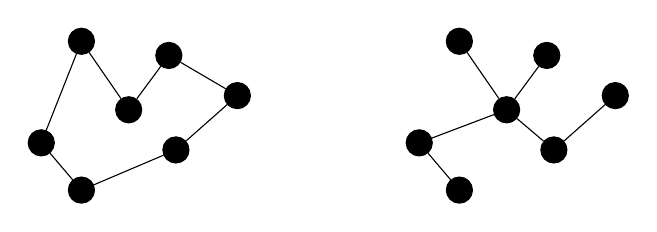
\begin{tikzpicture}[scale=0.6]
    \foreach \x in {0, 8}
  {
    \pgfmathsetmacro{\noise}{0.15}           
\node[draw,circle,fill=black] (1\x) at (\x+0, 0) {};
\node[draw,circle,fill=black] (2\x) at (\x+2, 1-\noise) {};
\node[draw,circle,fill=black] (3\x) at (\x+3+2*\noise, 2) {};
\node[draw,circle,fill=black] (4\x) at (\x+2-\noise, 3-\noise) {};
\node[draw,circle,fill=black] (5\x) at (\x+1, 2-2*\noise) {};
\node[draw,circle,fill=black] (6\x) at (\x+0, 3+\noise) {};
\node[draw,circle,fill=black] (7\x) at (\x-1+\noise, 1) {};
}

% TSP Solution
\foreach \a in {1,...,6}
  {
    \pgfmathsetmacro{\n}{int(\a+1)}
    \draw[-] (\a0) -- (\n0);
  }

\draw[-] (70) -- (10);

% Minimum spanning tree

\draw[-] (18) -- (78);
\draw[-] (28) -- (58);
\draw[-] (38) -- (28);
\draw[-] (48) -- (58);
\draw[-] (58) -- (68);
\draw[-] (78) -- (58);

  \end{tikzpicture}
\caption{巡回セールスパーソンにおけるTSP解 (左)と最小全域木 (右)}
\label{fig:tsp-mst}
\end{figure}


\section{非最適解の探索}
\label{sec:inadmissible}

許容的なヒューリスティックを用いたA*探索は最適解が得られるが、必ずしも最適解がほしいわけではない場合もある。解のクオリティよりもとにかく解が何か欲しい、という場合もある。
最適解ではない解を\define{非最適解}{suboptimal solution}{ひさいてきかい}と呼び、最適解に限らず解を発見するアルゴリズムを\define{非最適探索}{suboptimal search}{ひさいてきたんさく}と呼ぶ。% あるいは\define{局所探索}{local search}と呼ぶ。 % 局所探索はまた違う文脈か

\subsection{重み付きA*探索 (Weighted A*)}
\label{sec:weighted-astar-search}

\define{重み付きA*探索}{weighted A*}{おもみつきエースターたんさく} (wA*)は解のクオリティが落ちる代わりにより素早く解にたどり着くための手法である \cite{wilt2010comparison}。
wA*は重み付き$f$値、$f_w$が最小のノードを優先して探索する。

\begin{equation}
	f_w(u) = g(u) + w h(u)
\end{equation}

\dtheorem{
許容的なヒューリスティックを用いた重み付きA*探索によって発見される解は最適解のコスト$f^*$の$w$倍以下である。
}


wA*の利点はA*よりもはるかに高速であることである。
多くの場合、$w$の大きさに対して指数的な高速化が期待できる。これは深さ$d$のノードの個数は$d$に対して指数的(分枝度を$b$とすると$b^d$個)であることに対応する。

wA*などの非最適探索を使う場合はいずれにせよ最適解が得られないので、許容的でないヒューリスティックと組み合わせて使われることが多い。許容的でないヒューリスティックは許容的なヒューリスティックよりも高速であることが多い。% TODO lama?

wA*の解は最適解のコストの上界になるので、A*探索の枝刈りに用いることが出来る。
A*探索を実行する前にwA*を走らせ、解の上界$c^*$を得、A*探索実行時にノード$u$に対して$f$値が$f(u) \geq c^*$である場合、そのノードを枝刈りすることができる。このテクニックは多重配列アライメントなどに使われる\cite{ikeda1999enhanced}。

図\ref{fig:grid-astar}、\ref{fig:grid-wastar}はグリッド経路探索問題でのA*とwA* ($w=5$)の比較である。
緑のグリッドが初期位置、赤のグリッドがゴール、黒のグリッドは進行不可能の壁である。
青のグリッドが探索終了時点に各アルゴリズムによって展開されたノード、薄緑のグリッドが各アルゴリズムに生成され、まだ展開されていないノード (オープンリストにあるノード)である。

wA*の展開・生成ノード数がA*よりも少ない。
ただしwA*で発見された解はA*で発見された解よりも遠回りなことがわかる。
A*探索は最適解を発見するが、wA*では最初に発見した解が最適とは限らない。

\begin{figure}
  \centering
  \subfloat[A*] {
    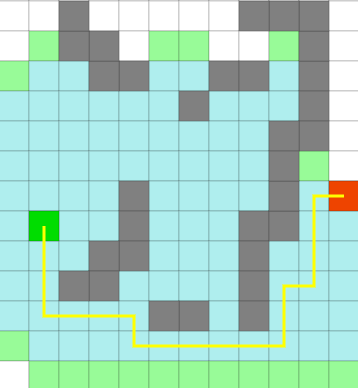
\includegraphics[width=0.3\linewidth]{./figures/grid-astar.png}
    \label{fig:grid-astar}
  } \hspace{4pt}
  \subfloat[wA*] {
    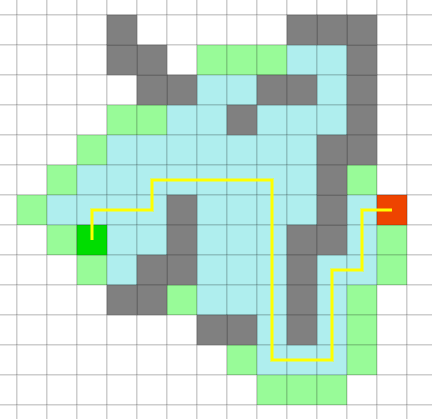
\includegraphics[width=0.3\linewidth]{./figures/grid-wastar-5.png}
    \label{fig:grid-wastar}
  } \hspace{4pt}
  \subfloat[GBFS] {
    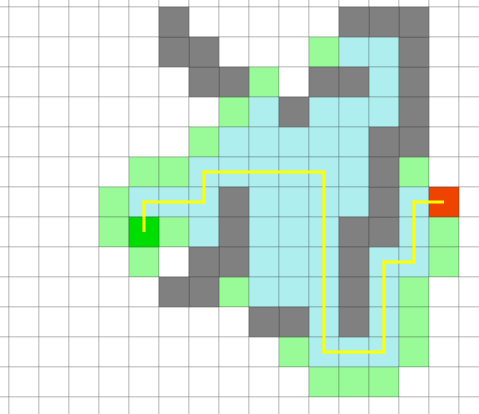
\includegraphics[width=0.3\linewidth]{./figures/grid-gbfs.png}
    \label{fig:grid-gbfs}
  }
  \caption{グリッド経路探索問題におけるA*、wA*、GBFSの比較}
  \label{fig:grid-comparison}
\end{figure}

\subsection{貪欲最良優先探索 (Greedy Best-First Search)}
\label{sec:greedy-best-first-search}

wA*の例で見たように、$g$値に対して$h$値に重きを置くことによって解のクオリティを犠牲により高速に解を得ることができる。
問題によっては解のクオリティはあまり重要でなかったり、そもそもクオリティという概念がないことがある。
このようにとにかく解があればよいという場合は\define{貪欲最良優先探索}{Greedy Best-First Search}{どんよくさいりょうゆうせんたんさく}が使われることが多い \cite{wilt2010comparison}。

\begin{equation}
  f_{\text{gbfs}}(u) = h(u)
\end{equation}

貪欲最良優先探索は$g$値を無視し、$h$値のみで展開順を決定する。つまりwA*の$w$を無限大にしたものである。

貪欲最良優先探索は解のクオリティに保証がない。
しかし多くの問題で高速に解を発見できるとても強力な手法である。
図\ref{fig:grid-gbfs}は貪欲最良優先探索である。wA*よりもさらに生成ノード数が少ないことが分かるだろう。

\subsection{山登り法 (Hill Climbing)}
\label{sec:hill-climbing}

A*探索はクローズドリストに探索済みのノードを記憶しておくことでグラフ全体を見渡して探索を進める。しかし探索済みのノードをメモリにおいておくことは時間がかかるし、メモリも消費する。\define{局所探索}{local search}{きょくしょたんさく}は現在見つかった最良のノードのみを記憶しておくことで効率的に(最適とは限らない)解を発見する方法である\footnote{局所探索の定義は分野によってさまざまである。例えば最適化問題を扱う分野ではある解から次の解を発見し、よりクオリティの高い解を発見していく手法を指すことが多い。}。

\define{山登り法}{hill climbing}{やまのぼりほう}は局所探索アルゴリズムであり、特に組み合わせ最適化問題のためのアルゴリズムとして使われる。
山登り法のアルゴリズムは非常に単純である。子ノードのうち最も$h$値が小さいノードを選ぶことを繰り返す。

\begin{algorithm}
\caption{山登り法 (Hill Climbing)}
	\Input{非明示的状態空間グラフ $(\mathcal{E}, u_0, \mathcal{G}, w)$, 評価関数 $h$}
	\Output{$u_0$からゴール状態への経路、経路が存在しなければ$\emptyset$}
	$u \leftarrow u_0$\;
	\While {{\bf not} $\mathcal{G}(u)$} {
	  $v \leftarrow \arg \min_{u' \in \mathcal{E}(u)} h(u')$\;
          $parent{v} \leftarrow u$\;
          $u \leftarrow v$\;
	}
	\Return $Path(u)$
\label{alg:hill-climbing}
\end{algorithm}

この手法は組み合わせ最適化・連続最適化のためによく使われる。
しかしグラフ探索アルゴリズムでこのまま使おうとすると評価関数の極小ではまってしまったり、デッドエンドに落ちてしまう可能性がある。


\subsection{強制山登り法 (Enforced Hill Climbing)}

ヒューリスティック探索でよく使われる局所探索は\define{強制山登り法}{enforced hill-climbing}{きょうせいやまのぼりほう} (EHC)である \cite{hoffmann2005ignoring}。
EHCは幅優先探索を繰り返し、現在のノードよりも$h$値が小さいノードを発見する。発見できればそのノードから再び幅優先を行い、ゴールを発見するまで続ける。もし$h$値が小さいノードが見つからなければ極小に陥ってしまったということであるので、探索を打ち切り、失敗 (Fail)を返す。

\begin{algorithm}
\caption{強制山登り法 (Enforced Hill Climbing)}
	\Input{非明示的状態空間グラフ $(\mathcal{E}, u_0, \mathcal{G}, w)$, 評価関数 $h$}
	\Output{$u_0$からゴール状態への経路、経路が存在しなければ$\emptyset$}
	$u \in u_0$\;
	\While {{\bf not} $\mathcal{G}(u)$} {
	  $R \leftarrow \mathcal{E}(u)$\;
	  $R' \leftarrow \{v \in R | h(v) < h(u) \}$\;
    \While {$R' = \emptyset$} {
      $R \leftarrow \{v \in \mathcal{E}(u') | u' \in R\}$\;
 	    $R' \leftarrow \{v \in R | h(v) < h(u) \}$\;
    }
	  $v \leftarrow \arg \min_{u' \in \mathcal{E}(u)} h(u')$\;
    $parent(v) \leftarrow u$\;
    $u \leftarrow v$\;
	}
	\Return $Path(u)$
\label{alg:hill-climbing}
\end{algorithm}


ほとんどの局所探索アルゴリズムは完全性を満たさない。
なので解が発見できなければ(失敗を返す場合)続けてA*探索などを走らせないと解が発見できない場合がある。
山登り法などの局所探索の利点はなんといってもオープンリストなどのデータ構造を保持する必要がないので消費メモリ量が非常に少ないことである。
またアルゴリズムがシンプルなため、実装が簡単であることも有用である。

山登り法が記憶しなければならないノードは現在のノードとその子ノードらだけである。
毎回次のノードを選択したら、そのノード以外のノードは捨ててしまう。
貪欲最良優先探索(\ref{sec:greedy-best-first-search}節)も同様に$h$値のみしか見ていないが、すべての生成済みノードをオープンリストに保存して評価値を確認していることと比較すると、山登り法がいかにアグレッシブな手法であるかがうかがえるだろう。

\section{上手く行かない場合}

ヒューリスティック探索が思ったより遅い場合考えるべきことはいくつかある。

まず考えるべきは、そもそもヒューリスティック探索によって解くべき問題なのかという点である。
制約プログラミングや他の組合せ最適化手法なら効率的な問題かもしれない。
似たような問題が他の手法によって解かれていないかを調べてみると良い。

ヒューリスティック探索が良さそうだと思ったら、試しにwA*にしてみて、weightを大きく取ってみよう。
おおまかに言うとwA*の実行速度はwの大きさに対して指数的に速くなる。$w=1$だと全く解けそうにない問題でも$w=2$にすると一瞬で解けることがある。
もし$w$を10くらいにしてもすぐに解が発見できなければ、おそらくその問題で最適解を発見するのは非常に難しい。このような問題に対しては最適解を見つけることは諦め、非最適解探索 (節 \ref{sec:inadmissible})を使ったほうが良いだろう。
wA*でも解が見つけられない場合はそもそも解がない問題かもしれない。実は解がない状態空間問題において解がないことを証明することは非常に難しいことである。ヒューリスティック探索分野でもいくつかアプローチがある \cite{backstrom2013fast,eriksson2017unsolvability}が、他のアプローチを試した方が良いだろう。

wA*で非最適解を見つけられる場合なら、工夫すればA*で最適解を見つけることができるかもしれない。
その場合まず、おおまかな探索空間の大きさを見積もり、そして1秒間に何ノードが展開されているかを確認すると良い。
ヒューリスティック探索の実行時間はおおまかには(展開するノード数)と(1ノードの展開にかかる時間)の積である。

%例えばA*探索はC++でスライディングタイル問題だと秒間XXXノードが展開できる。
もし秒間に展開されているノードの数が少ない場合、プロファイラを使ってどのオペレーションに時間がかかっているかを確認するべきだろう。多くの場合実行時間の大半をオープンリスト、クローズドリスト、ノードの展開関数(現在の状態とアクションから状態を計算する関数)のいずれかが占めている、ということがわかるだろう。

オープンリスト、クローズドリストの処理に時間がかかっている場合はデータ構造の改良によって問題が解決するかもしれない。効率的なデータ構造の設計については\ref{ch:search-performance}章を参照されたい。
特に探索が進みデータ構造が大きくなるほどアクセスするためにかかる時間がどんどん増えていく場合はデータ構造の工夫によって解決できる可能性がある。
あとはプロセスのメモリ消費量を確認してみよう。A*はメモリ消費も激しい。
実行時間が遅いのは、メモリを使いすぎていてメモリスワップが起きているからかもしれない。
より大きなメモリを使うか、IDA*などのメモリの消費量の少ない手法を試してみると良いかもしれない。

ノードの展開関数に時間がかかる場合はその実装を工夫するか、ノードの展開回数を最小限に抑えるしかない。
ノードの展開回数を減らす方法はなかなか難しいが、例えばヒューリスティック関数の改良によって可能である。
ほんの少しのヒューリスティック関数の改善によって探索の効率は劇的に上がりうる。
% 例えばスライディングタイル問題ではTODO。

これらの方法でもまだ解けない場合、扱っている問題は純粋なA*で解くには結構難しい問題かもしれない。
1968年にA*が初めて提案されてから、様々な発展手法が考案されてきた。
本書の後半で紹介する最新の手法を試してみれば解けるかもしれない。




\section{関連文献}

\define{最良優先探索}{best-first search}{さいりょうゆうせんたんさく}は2種類の定義があることに注意したい。
本書では最良優先探索をA*を含む、何らかの有望さの指標に従ってグラフを探索するアルゴリズムを指す。
一方、ゴールに最も近いと考えられるノードを常に最優先して展開するアルゴリズムを特に最良優先探索と呼ぶことも多い。本書ではこの方法は貪欲最良優先探索と呼んでいる。


制限時間内でできるだけ良いクオリティの解が欲しい場合はAnytime Reparing A* \cite{likhachev2004ara}が使える。Anytime Reparing A*は問題に対して重み付きA*を繰り返し$w$値をだんだんと小さくしていくことでだんだんと解のクオリティを向上させる。一般にいつ停止しても現時点で見つかった中で一番良い (最適とは限らない)解を返し、時間をかけるほど解のクオリティを改善していくアルゴリズムをanytimeアルゴリズムと呼ぶ。Anytimeアルゴリズムとしては他にもモンテカルロ木探索などがある \cite{browne2012survey}。

山登り法は評価値が最も良い状態を決定論的に選ぶので解・最適解を発見する保証はない。
一方、すべての次状態を均等な確率でランダムに選ぶランダムウォークはいずれ解を発見するが、時間がかかりすぎる。
\define{焼きなまし法}{simulated annealing}はこの二つの手法の中間をとったような手法であり、最初は評価値を無視して均等なランダムウォークからはじめ、探索が進行していくにつれて評価値に応じて次状態を選択するようにするという手法である \cite{vcerny1985thermodynamical,van1987simulated}。焼きなまし法は最適化問題で非常に重要なアルゴリズムである \cite{kirkpatrick1983optimization}。

\define{遺伝的アルゴリズム}{genetic algorithm}もさまざまな最適化問題に適用できる重要なアルゴリズムである \cite{goldberg1989}。
グラフ探索問題で使われることは少ないが、グラフ探索問題ではなかなか解けない難しい問題が遺伝的アルゴリズムによって簡単に解けることがある。例えばN-Queen問題はチェスの盤面上にクイーンを互いに移動可能範囲がぶつからないように配置する問題であるが、これはグラフ探索の手法だとなかなか解くのが難しいが遺伝的アルゴリズムだと非常に効率的に解けることが知られている。


% -*- coding: utf-8 -*-
\chapter{グラフ探索のためのデータ構造}
\label{ch:search-performance}

ヒューリスティック探索の効率は探索効率、つまり展開したノードの数によって測られる場合が多い。本書の多くの節は探索効率を上げるためのアルゴリズムについて解説している。
しかしヒューリスティック探索の実行時間とメモリ量はデータ構造の実装にも大きく左右される。

ヒューリスティック探索ではオープンリストとクローズドリストの2つのデータ構造を保持する。
オープンリストに必要なインターフェイスは必要な操作はエンキュー (enqueue, pop)とデキュー (dequeue, push)である。
クローズドリストに必要なインターフェイスは挿入 (insert)と重複検知のための検索 (find, lookup)である。

これらのデータ構造をどのように実装するかは探索の効率に大きな影響を与える。
歴史的な経緯からオープン・クローズドリストと呼ばれているが、リストとして実装するのは非効率的である。

これらを実装するための効率的なデータ構造はアルゴリズムと問題ドメインに依存する。
この章ではどのようなシチュエーションでどのようなデータ構造を使われるかを説明する。
この章は実践的に非常に重要な章である。
残念ながらヒューリスティック探索の研究論文のほとんどはこの章で扱われる内容について自明のものとして扱わない。あるいはこれらの内容を「コードの最適化」として論文中には明示しない。が、その実自明ではないので初学者の多くはここで苦労することになる。
データ構造について議論を行っている論文としては\cite{burns2012implementing}がある。

%まず、$f$値の定義域が連続値か離散値かは重要である。
%また、$f$値が単調増加するかどうか。これはヒューリスティックが無矛盾かどうかにも依存する。



\section{オープンリスト (Open List)}
\label{sec:open-list}
%\captionlistentry[todo]{openlist}
オープンリストのプライオリティキューの実装方法は様々ある。
$f$値が連続値 (e.g. 実数)である場合はヒープを使うことが多い。
$f$値の取りうる値が有限個であり、$f$値が同じノードが沢山ある場合はバケットで実装することが出来る。
また、そのような場合は$f$値が同じノードのうちどのノードを選ぶかの\define{タイブレーキング}{tiebreaking}{タイブレーキング}も重要になってくる。


\subsection{データ構造の選択}
\label{sec:priority-queue}

オープンリストは探索の中で沢山エンキューとデキューを行うため、これらの操作の計算時間が速いものを選択したい。
オープンリストのシンプルな実装方法としては二分ヒープがあげられる。二分ヒープはほとんどの言語の標準ライブラリにあるため実装が簡単である。
探索アルゴリズムはノードの数が膨大になることが多い。
計算量のオーダーで見ると単純な二分ヒープよりも\define{フィボナッチヒープ}{Fibonacci heap}{フィボナッチヒープ}が効率が良いが、定数項が大きいため多くの場合二分ヒープが採用される。
二分ヒープよりも効率が良いデータ構造として\define{基数ヒープ}{radix heap}{きすうヒープ}がある \cite{ahuja1990faster}。基数ヒープはエンキューできる数値は最後に取り出した数値以上のものであるという制約がある。A*探索はヒューリスティックが単調である場合この制約を満たす。
これらのヒープの実装や性質についてはIntroduction to Algorithmsを参照されたい \cite{cormen01}。

プライオリティ値が取る値が有限個である場合はバケットで実装をすることが出来る \cite{burns2012implementing}。プライオリティ値が取る値が$C_{min} \leq i \leq C_{max}$の整数値であるとする。
バケットは長さ$C_{max} - C_{min} + 1$の配列からなる。プライオリティ値が$i$の要素は配列の$i - C_{min}$番目の位置にあるリストに追加される。バケットはエンキューもデキューも$O(C_{max} - C_{min})$で計算でき、保持しているノードの数に依存しない。そのため二分ヒープよりも高速であることが多い。
後述するタイブレーキングを行う場合はバケットの中に更に二段階目のバケットを用意することもできる \cite{burns2012implementing}。

\begin{figure}
  \centering
  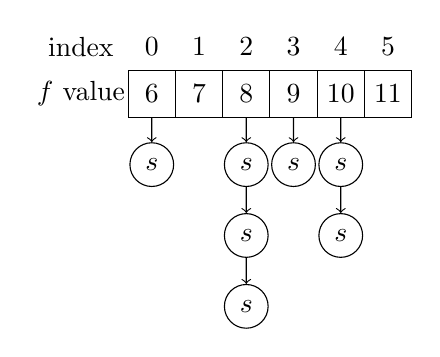
\begin{tikzpicture}[scale=0.6]
    % Array
\draw (0, 0) grid (6, 1);

% f-value and index
\foreach \x in {0, 1, ..., 5} {
  \pgfmathsetmacro{\fval}{int(\x + 6)}
  \node (f\x) at (\x + 0.5, 0.5) {\fval};
  \node (i\x) at (\x + 0.5, 1.5) {\x};
}

% label
\node (f) at (-1, 0.5) {$f$ value};
\node (i) at (-1, 1.5) {index};


% items
\node at (0 + 0.5, -1) [circle, draw] (n01) {$s$};
\draw[->] (0 + 0.5, 0) -- (n01);

\node at (2 + 0.5, -1) [circle, draw] (n21) {$s$};
\node at (2 + 0.5, -2.5) [circle, draw] (n22) {$s$};
\node at (2 + 0.5, -4) [circle, draw] (n23) {$s$};
\draw[->] (2 + 0.5, 0) -- (n21);
\draw[->] (n21) -- (n22);
\draw[->] (n22) -- (n23);

\node at (3 + 0.5, -1) [circle, draw] (n31) {$s$};
\draw[->] (3 + 0.5, 0) -- (n31);

\node at (4 + 0.5, -1) [circle, draw] (n41) {$s$};
\node at (4 + 0.5, -2.5) [circle, draw] (n42) {$s$};
\draw[->] (4 + 0.5, 0) -- (n41);
\draw[->] (n41) -- (n42);


  \end{tikzpicture}
  \caption{バケットによるオープンリストの実装 ($C_{min} = 6$, $C_{max} = 11$)}
  \label{fig:bucket}
\end{figure}


\subsection{タイブレーキング (Tiebreaking)}
\label{sec:tiebreaking}

\ref{ch:blind-search}章、\ref{ch:heuristic-search}章ではオープンリストでどのノードを最初に展開するかによってアルゴリズムの性能が大きく変わることを示してきた。
例えばA*探索では$f$値が最小のノードを優先して展開する (アルゴリズム\ref{alg:astar-search})。
だが、$f$値が最小のノードは複数ある場合がある。コスト関数が離散値である場合は$f$値が同じノードが大量にあることが多い。
このような場合、同じ$f$値のノードの中からどのノードを選ぶかを決定することを\define{タイブレーキング}{tie-breaking}{タイブレーキング}と呼ぶ。

A*探索で広く使われるタイブレーキング戦略は$h$値が小さいノードを優先させる方法である。$\arg \min_{u' \in Open} f(u')$を選択する代わりに以下の条件を満たす$u$を選択する。

\begin{align*}
  u =& \arg \min_{v \in B} h(v) \\
  s.t. \; \; & B = \{v | v \in Open, f(v) = \min_{v' \in Open} f(v')\}
\end{align*}

$h$値が小さいノードを優先させる理由としては、$h$値がゴールへの距離の推定だからである。なのでゴールに近いノードから展開したほうがゴールにたどり着くのが早いはずだ、というヒューリスティックである。

もう一つはLast-in-first-out (LIFO)タイブレーキングがよく使われる。
LIFOは最後にオープンリストに入ったノードから優先して展開する。
LIFOを使うメリットはオープンリストをバケット実装している場合に配列の一番後ろのノードがLIFOで得られるノードであることである。
\ref{sec:priority-queue}節にあるようにバケットは配列で実装されることが多いが、配列の末尾のノードを取り出すには定数時間しかかからない。なので自然にバケットを実装するとLIFOになる。

%逆にFirst-in-first-out (FIFO)にすると

タイブレーキングは長い間ヒューリスティック探索研究の中であまり重要視されておらず、よいヒューリスティック関数をデザインすることと比較してアルゴリズムの効率に対してあまり影響を及ぼさないと考えられてきた。
近年の研究でタイブレーキングが重要なファクターになる場合があるということが実験的に示された \cite{asai2016tiebreaking}。


\section{クローズドリスト (Closed List)}
\label{sec:closed-list}

重複検出は無駄な展開を防ぐために不可欠な操作である。
非明示的状態空間グラフではあらかじめすべての状態を知ることが出来ないので、探索中に発見された状態の集合を保持しておくための動的な辞書が必要になる。

クローズドリストは生成済み・展開済みノードを保持し、新しくノードが生成されたときにすでにその中にあるかどうかを確かめる。
一般的に辞書のデータ構造は挿入 (insert)、検索 (lookup)、削除 (delete)をサポートするが、探索アルゴリズムに必要なのは挿入と検索である。

クローズドリストの実装には\define{ハッシュテーブル}{hash table}{ハッシュテーブル}が用いられることが多い。
ハッシュテーブルは探索で一番頻繁に使われる検索が定数時間で出来るためである。


\subsection{ハッシュテーブル (Hash Table)}
\label{sec:hash-table}

集合$U = \{0, 1, ..., N - 1\}$をキーの候補とする\define{辞書}{dictionary}{じしょ}は、保持されたキーの集合$R \subseteq U$から連想情報の集合$I$への部分写像である。
グラフ探索において状態$s \in S$を一意に表すためのキーを$k(s)$とする ($k: S \rightarrow U$)。
キーは更にハッシュテーブルと呼ばれる配列$T[0, ..., m-1]$に写される。この写像$h: U \rightarrow \{0, ..., m-1\}$を\define{ハッシュ関数}{hash function}{ハッシュかんすう}と呼ぶ。簡単のためここでは状態から配列のインデックスまでの関数$S \rightarrow \{0, ..., m-1\}$を$h$を使って表す。

多くの場合$N > m$なので、このハッシュ関数は単射ではない。よって異なるキーがハッシュテーブル上の同じ位置に配置されることになる。これをハッシュの\define{衝突}{hash collision}{しょうとつ}と呼ぶ。
ハッシュテーブルへのアクセスにかかる時間は1. ハッシュ値の計算、2. 衝突時の処理方法、3. 保持されたキーの数とハッシュテーブルの大きさの比に依存する。

ハッシュ関数の選択はハッシュテーブルの性能に大きく影響を与える。最悪の場合、すべてのキーがテーブルの同じ位置に移される。最良の場合、一度も衝突が起こらず、アクセス時間は定数になる。最悪の場合の計算時間は理論的には興味のある話題だが、多くの場合正しくハッシュを計算することで避けられる。

衝突したハッシュの処理方法としては\define{連鎖法}{chaining}{れんさほう}と\define{開番地法}{open addressing}{かいばんちほう}がある。連鎖法はハッシュテーブルの各位置にリストが置かれ、その位置に挿入された連想情報はそのリストに順次追加されていく。同じ位置に$n$個の状態が挿入された場合リストの長さは$n$になる。このとき、ここの位置への検索の速度は$O(n)$となる。開番地法は衝突した場合テーブル中の空いている別の位置を探し、そちらに入れる方法である。探索アルゴリズムにおいては連鎖法が使われることが多い。


\subsection{ハッシュ関数 (Hash Function)}
\label{sec:hash-function}

{\bf 良い}ハッシュ関数に求められる要件は主に2つである。
一つはハッシュ値が値域内でなるべく均等に分散してほしい。
もう一つはハッシュの計算に時間がかからない方が良い。

グラフ探索のためのハッシュ関数をデザインするために考えなければならないのは、探索中に現れる状態集合、探索空間は状態空間全体のほんの一部であり、かつ偏りのある集合であるということである。
ハッシュ関数はその探索空間内でハッシュ値が十分に均等であってほしい。


\subsubsection{剰余法 (Remainder Method)}

$k(s)$を整数と考えることが出来るならば、それを$m$で割った余りをハッシュ値として使える。

\begin{equation}
  h(s) := k(s) \; \text{mod} \; m
\end{equation}
  
このハッシュ関数は$S$から$T$への写像になる ($h: S \rightarrow \{0, ..., m-1\}$)。$T$へ均等に分配するためには法$m$の選択が重要になる。
例えば$m$に2の倍数を選んでしまうと、$h(s)$が偶数であるのは$k(s)$が偶数であるときであり、そのときのみである (iff)。$m$が任意の数の倍数であると同様の不均一が起きてしまうので、$m$は素数を選ぶと良い。


\subsubsection{積算ハッシュ法 (Multiplicative Hashing)}
積算ハッシュ法はキー$k(s)$と無理数$\phi$の積の小数部分を使ったハッシュである。

\begin{equation}
	h(s) = \floor{m (k(s) \phi - \floor{k(s) \phi})}
\end{equation}

$\phi$はパラメータであり、$(\sqrt{5} - 1) / 2$の黄金比を使うと良いとされている。

\subsubsection{ハッシュの性質}

関連して、クローズドリストにとって良い性質のハッシュがいくつかある。

グラフ探索では状態遷移は状態の一部分のみに作用し、状態変数のほとんどは変わらないということが多い。このとき、新しい状態のハッシュ値を一から計算するのではなく、元の状態のハッシュ値と状態遷移による差分を利用して新しい状態のハッシュ値を求めることが出来る場合がある。この方法を\define{差分ハッシュ}{incremental hashing}{さぶんハッシュ}と呼ぶ。差分ハッシュはハッシュ値の計算時間を短くできることがある。

どのような操作があっても衝突が起こらないようなハッシュを\define{完全ハッシュ}{perfect hash function}{かんぜんハッシュ}と呼ぶ。もし$n = m$であれば最小完全ハッシュと呼ぶ。完全ハッシュがあればどのような操作も$O(1)$で行うことができる。
問題によって完全ハッシュは簡単に計算することが出来る。例えばスライディングタイルパズルであれば状態$s = (v_0, v_1,...,v_8)$に対して$h(s) = \sum_{i = 0..8} v_i \cdot 9^i$と単純に状態変数の列を使って計算することが出来る。ただし長さ$9^9$の配列は大きすぎるので工夫が必要になる。完全ハッシュを作るのは簡単だが、小さい完全ハッシュを作るのは難しい。スライディングタイルパズルは\define{辞書順}{lexicographical order}{じしょじゅん}によって最小完全ハッシュを作ることが出来る \cite{korf2005large}。


\subsection{トランスポジションテーブル (Transposition Table)}

木探索の問題点は重複検出を行わないため、同じ状態を複数回展開し、時間がかかってしまうことである。一方グラフ探索の問題点は重複検出を行うため、生成したノードの数だけメモリを消費することにある。
グラフが大きい場合はやがてメモリを使い果たし、探索が続けられなくなってしまう。
しかしながら、実はグラフ探索において重複検出は必ずしも正しくなければならないものではない。重複してノードを生成しても問題なくアルゴリズムは動作する。仮にクローズドリストの一部を捨ててもアルゴリズムの正しさを損なうものではない。

\define{トランスポジションテーブル}{transposition table}{トランスポジションテーブル}はこのアイディアに基づき、展開したノードの一部のみを保存することで重複検出をしつつメモリの消費を抑える手法である。
トランスポジションテーブルはグラフ探索におけるクローズドリストと同様、辞書である。
クローズドリストがすべての生成済みノードを保持していることを保証するのに対して、トランスポジションテーブルはそのような保証をしない。
トランスポジションテーブルはどのノードを保持し、どのノードを捨てるかを賢く選択しなければならない。どのノードを保持するべきかという戦略はいくつか提案されている \cite{breuker1994replacement,akagi2010transposition}。

単純なものとしては、テーブルが一杯になるまではすべてのノードをテーブルに追加し、テーブルが一杯になったらすべてのノードを捨てる戦略がある。
Stochastic node caching \cite{miura1999stochastic}は、新しく追加されたノードを確率$1-p$で捨てるというものである。この戦略だと$n$回訪れたノードは確率$1- (1-p)^n$でテーブルに追加されるため、たくさん訪れたノードほど重複検出されやすいことになるという点で合理的である。
2人ゲームでよく使われる戦略は、2つのノードのハッシュ値が衝突したらどちらか一方のみを残すという戦略である。より$d$値が大きい(深い)ノードを残す戦略が一般的である。この戦略はハッシュテーブルの衝突を減らせるという点で一挙両得になる。

トランスポジションテーブルはA*だけでなく後述するIDA* (節\ref{sec:depth-first-iterative-deepening})でも使われる \cite{reinefeld1994enhanced}。IDA*の空間量は最適解の深さに対して線形なので消費メモリが非常に少ない。あまったメモリを効率よく使うためにIDA*にトランスポジションテーブルを用いるという研究が多い \cite{reinefeld1994enhanced,akagi2010transposition,kishimoto:02}。

トランスポジションテーブルは元々2人ゲームの分野から発展した技術である。同じ手を異なる順番で行うことで同じ状態に到達することを検出するために使われていたのでtranspositionという名前になっている。


\subsection{遅延重複検出 (Delayed Duplicate Detection)}
\label{sec:delayed-duplicate-detection}

\ref{sec:graph-search-algorithm}節ではノードを生成したタイミングで重複検出を行うアルゴリズムを説明した。この方法だとノードが生成されたその瞬間に検出を行うという意味で\define{即時重複検出}{immediate duplicate detection}{そくじちょうふくけんしゅつ}と呼ぶことがある。
それに対して、ノードを展開するタイミングで検出を行う\define{遅延重複検出}{delayed duplicate detection}{ちえんちょうふくけんしゅつ}という方法もある \cite{korf12003delayed}。
ノードが生成された瞬間に重複検出を行わない場合、オープンリスト内に同じ状態を持ったノードが重複して存在する場合がある。
しかしノードを展開するときに重複検出を行うので、クローズドリストにノードの重複はない。
アルゴリズム\ref{alg:ddd}は遅延重複検出を用いる場合のグラフ探索アルゴリズムの疑似コードである。

遅延重複検出は展開ノード毎に重複検出の回数を減らすことができるというメリットがある。一方、オープンリスト内に重複が存在する可能性があるため、プライオリティの選択次第ではノードの再展開が増えてしまうデメリットがある。
そのため遅延重複検出はノードの重複が少ない問題や、重複検出に時間がかかる場合に使われる。特にクローズドリストをハードディスクなどの外部メモリに置く外部メモリ探索に相性が良い。


\begin{algorithm}
\caption{遅延重複検出を用いたグラフ探索}
\label{alg:ddd}
	\Input{非明示的状態空間グラフ $(s, Goal, Expand, w)$, プライオリティ関数 $f$}
	\Output{$s$からゴール状態$t \in T$への経路、経路が存在しなければ$\emptyset$}
	$Closed \leftarrow \emptyset$, $Open \leftarrow \{s\}$, $d(s) \leftarrow 0$, $g(s) \leftarrow 0$\;
	\While{$Open \neq \emptyset$} {
                $u \leftarrow \argmin_{u' \in Open} f(u')$ \;
	        $Open \leftarrow Open \setminus \{u\} $\;
          
		\If {$Goal(u)$} {
			\Return $Path(u)$\;
		}

                $s \leftarrow parent(u)$\;
		\If{$u \notin Closed$ {\bf or} $g(s) + w(s, u) < g(u)$} {
                  $d(u) \leftarrow d(s) + 1$\;
                  $d(u) \leftarrow g(s) + w(s, u)$\;
		  $parent(u) \leftarrow s$\;
		  \For {each $v \in Expand(u)$} {
		    $Open \leftarrow Open \cup \{v\}$\;
		    $parent(v) \leftarrow u$\;
		  }
		}

                \If{$u \notin Closed$} {
                  $Closed \leftarrow Closed \cup \{u\}$\;
                }
 	}
	\Return $\emptyset$\;
\end{algorithm}


\subsection{関連文献}

\TODO{Rabin and Karp hashing}

\TODO{Universal hash function}




% -*- coding: utf-8 -*-
\chapter{時間・空間制限下のヒューリスティック探索}
\label{ch:heuristic-search-variants}


A*探索などのヒューリスティック探索は時間と空間の両方がボトルネックとなりうる。
すなわち、A*はノードを一つずつ展開していかなければならないので、その数だけExpandを実行しなければならない。また、A*は重複検出のために展開済みノードをすべてクローズドリストに保存する。なので、必要な空間も展開ノード数に応じて増えていく。

残念ながら、ほぼ正しいコストを返すヒューリスティック関数を使っても、A*が展開するノードの数は指数的に増加することが知られている\cite{helmert:08}。

そのため、ヒューリスティックの改善のみならず、アルゴリズム自体の工夫をしなければならない。
この章では時間・空間制約がある場合のA*の代わりとなるヒューリスティック探索の発展を紹介する。
これらのアルゴリズムはメリット・デメリットがあり、問題・計算機環境によって有効な手法が異なる。よって、A*を完全に取って代わるものは一つもないと言える。

\define{分枝限定法}{branch-and-bound}{ぶんしげんていほう}は非最適解を見つけやすい問題で特に有効な手法であり、メモリ消費が小さいというメリットがある。
\define{反復深化A*}{iterative deepening A*}{はんぷくしんかエースター}は線形メモリアルゴリズムであり、メモリが足りない問題で使われる。
\define{両方向探索}{bidirectional search}{りょうほうこうたんさく}は初期状態とゴール状態の両方から探索をはじめ、二方向の探索が交わるところを探す方法である。ヒューリスティック関数の精度が悪いときに有用である場合が多いことが知られている。
\define{シンボリック探索}{symbolic search}{シンボリックたんさく}は\define{二分決定グラフ}{Binary Decision Diagram}{にぶんけっていぐらふ}を用いて状態集合を表すことによってノードの集合に対して一度に演算を行う手法である。
新奇性に基づく枝刈りは目新しくない状態は枝刈りする。
% 外部メモリ探索は状態空間がメモリに収まりきらない問題に対して外部記憶を使うことで解決する手法である。
\define{並列探索}{parallel search}{へいれつたんさく}は複数のコアや計算機を使うことでメモリと計算時間の両方の問題を解決する。


\section{分枝限定法 (Branch-and-Bound)}
\label{sec:branch-and-bound}

\define{分枝限定法}{branch-and-bound}{ぶんしげんていほう}は非最適解が簡単に見つけられるが最適解を発見するのは難しい問題、例えば巡回セールスパーソン問題などに使われることが多い。
分枝限定法は広くコンピュータサイエンスで使われる汎用的な考え方である。
アイディアとしては問題を複数のサブ問題に分割(branch)し、これまでに得られた解よりも悪い解しか得られないサブ問題を枝刈りする(bound)、というアイディアである。
特にメモリ効率の良い深さ優先分枝限定法 (Depth-First Branch-and-Bound)が探索分野ではよく使われる。
分枝限定法の処理は一般的な木探索に加えて枝刈りが行う (アルゴリズム \ref{alg:branch-and-bound})。

% TODO
\begin{algorithm}
\caption{深さ優先分枝限定法 (Branch-and-Bound)}
\label{alg:branch-and-bound}
        \Input{非明示的状態空間グラフ $(s, Goal, Expand, w)$、ヒューリスティック関数 $h$}
	\Output{$s$からゴール状態$t \in T$への経路、経路が存在しなければ$\emptyset$}
	$U \leftarrow \infty$\;
	$path \leftarrow \emptyset$\;
	$(U, path) \leftarrow DFB\&B(s, 0, U, path)$\;
	\Return $path$\;
\end{algorithm}

\begin{algorithm}
\caption{DFB\&B(s, g, U, path): 分枝限定法の再帰計算}
\label{alg:branch-and-bound-rec}
	\If {$Goal(s)$} {
		\If {$g < U$} {
			$U \leftarrow g$\;
			$path \leftarrow Path(s)$\;
		}
	}
        \Else {
          $Succ(s) \leftarrow Expand(s)$, sorted according to $h$\;
	  \For {each $s' \in Succ(s)$} {
	    \If {$g + h(s') < U$} {
	      $(U, path) \leftarrow DFB\&B(v, g + w(s, s'), U, path)$\;
	    }
	  }
        }
        \Return $(U, path)$
\end{algorithm}

一般に、アルゴリズムの実行に従って最適解とは限らない解を次々と発見する手法において分枝限定法の考え方が採用できる。すなわち現在発見された中でもっとも良い解(incumbent solution)を用いて探索範囲を限定していくアイディアである。
A*探索と比較して分枝限定法の利点は、\define{任意時間アルゴリズム}{anytime algorithm}{にんいじかんアルゴリズム}であることである。
任意時間アルゴリズムとはプログラムを適当なタイミングで停止しても解を返すアルゴリズムを指す。
A*探索は最適解を発見するまで他の非最適解を発見することはない。一方、分枝限定法はすぐに何かしらの解を見つけることができる。そして探索の過程で現在の解よりも良い解を発見し、だんだんと解のクオリティを上げていき、最終的に最適解を発見する。
そのため、どのくらい長い間探索に時間をかけてよいかが分からない場合、任意時間アルゴリズムは理想的である。
関連して、A*のそのような問題を解決した\define{任意時間A*}{Anytime A*}{にんいじかんエースター}というアルゴリズムもある \cite{likhachev2004ara,hansen2007anytime,richter2010joy}。例えば単純にwA*において$w$の値を大きなものからだんだんと1に近づける方法がシンプルで効率的である。
A*や任意時間A*と比較した分枝限定法のもう一つの利点はオープンリストなどのデータ構造を必要としない深さ優先探索であることである。そのためメモリ・キャッシュ効率が良い。一方、重複検出を行わない木探索であるため、ノードの重複が多いドメインでは性能が悪いことが多い。


\section{反復深化深さ優先探索 (Depth First Iterative Deepening)}
\label{sec:depth-first-iterative-deepening}
A*探索は時間・空間の両方がボトルネックになるが、現代の計算機環境では多くの場合空間制約がよりネックになる。
これはA*が重複検出のために展開済みノードをすべてクローズドリストに保存していることに起因する。

\ref{sec:graph-search-algorithm}節で述べたように、重複検出は正しい解を返すためには必須ではない。グラフに対して木探索を行うことも出来る。
しかしながら、単純な幅優先木探索・深さ優先木探索はパフォーマンスの問題がある。

\define{反復深化深さ優先}{depth first iterative deepening}{はんぷくしんかふかさゆうせん} (DFID)は深さ優先探索もメモリ効率と幅優先探索の効率性を併せ持った賢いアルゴリズムである \cite{korf:85a,russelln03}。
アイディアとしては、閾値$cost$を1ずつ大きくしながら、繰り返しコスト制限付き深さ優先 (CLDFS)を実行する (アルゴリズム\ref{alg:depth-first-iterative-deepening})。CLDFSが解を見つければその解を返して停止し、見つけられなければ$cost$を1つ大きくしてもう一度CLDFSを実行する。

DFIDは閾値を大きくする度に一つ前のイテレーションで展開・生成したノードをすべて展開・生成しなおさなければならない。各イテレーション内でもクローズドリストを保持していないために重複検出が出来ない。なので、アルゴリズム全体を通して大量の重複ノードが出る可能性がある。
一見非常に効率が悪いように思えるかもしれないが、実はあまり損をしないことが多い。分枝数を$b$、最適解のコストを$c^*$とする。DFIDは$c^*$回目のイテレーションで生成するノードの数はおおよそ$1 + b + b^2 + ... + b^{c^*} = O(b^{c^*})$である。$c^* - 1$回目のイテレーションで生成されるノードの数はその数のおよそ$1 / b$倍である。$c^* - 2$回目のイテレーションではその更に$1 / b$倍と、指数的に生成ノード数は減っていく。そのため、DFID全体でノードを生成する回数は、$c^*$回目のイテレーションでノードを生成する回数とあまり変わらない。

DFIDのメリットはいくつかある。
まず、コスト$w$が0となるアクションが存在しない場合、必要なメモリ量が最適解のコストに対して線形である ($O(b c^*)$)。そのため、幅優先ではメモリが足りなくなって解けないような難しい問題でもDFIDなら解ける可能性がある。

メモリ量と関連してもう一つの重要なメリットはキャッシュ効率である。上述のようにDFIDは必要なメモリ量が非常にすくない。また、メモリアクセスパターンもかなりリニアである。そのため、ほぼキャッシュミスなく探索を行えるドメインも多い。例えば、スライディングタイルパズルなどの状態が少ないビット数で表せられるドメインでは特にキャッシュ効率が良く、1ノードの展開速度の差は圧倒的に速い\cite{korf:85a}。

DFIDは解を返す場合、得られた解が最適解であることを保証する。
DFIDをはじめとする重複検出のないアルゴリズムを用いる際の問題は、解がない場合に停止性を満たさないことである。問題に解がなく、グラフにループがある場合、単純な木探索は停止しない。よって、この手法は解が間違いなく存在することが分かっている問題に対して適用される。あるいは、解が存在することを判定してから用いる。
例えばスライディングタイプパズルは解が存在するか非常に高速に判定することが出来る。

\begin{algorithm}
\caption{反復深化深さ優先 (Depth First Iterative Deepening)}
\label{alg:depth-first-iterative-deepening}
        \Input{非明示的状態空間グラフ $(s, Goal, Expand, w)$}
	\Output{$s$からゴール状態$t \in T$への経路、経路が存在しなければ$\emptyset$}
        $U' \leftarrow 0$\;
        $path \leftarrow \emptyset$\;
        \While {$path = \emptyset$ {\bf and} $U' \neq \infty$} {
          $U \leftarrow U'$\;
          $(U', path) \leftarrow CLDFS-DFID(s, 0, U)$\;
        }
        \Return $path$\;
\end{algorithm}

\begin{algorithm}
\caption{CLDFS-DFID: DFIDのためのコスト制限付き深さ優先}
\label{alg:cldfs}
	\Input{状態 $s$、経路コスト $g$、閾値 $U$}
	\Output{$s$からゴール状態$t \in T$への経路、経路が存在しなければ$\emptyset$}
        $U' \leftarrow \infty$\;
	\If {$Goal(s)$} {
		\Return $(_, Path(s))$\;
	}
	\For {each $u \in Expand(s)$} {
		\uIf {$g + w(s, u) \leq U$} {
			$p \leftarrow CLDFS(u, g + w(s, u), U)$\;
			\If {$p \neq \emptyset$} {
				\Return $(s, p)$\;
			}
		}
                \uElseIf {$g + w(s, u) < U'$} {
                  $U' \leftarrow g + w(s, u)$\;
                }
	}
	\Return $(U', \emptyset)$\;
\end{algorithm}


\subsection{反復深化A* (Iterative Deepening A*)}
\label{sec:iterative-deepening-astar}


反復深化A* (IDA*)は木探索に対してヒューリスティックを用いた、非常にメモリ効率の良いアルゴリズムである \cite{korf:85a}。
DFIDと同様、コストを大きくしながら繰り返しCLDFSを呼ぶ。
ただし、DFIDでは$g$値によってコストを制限していたのに対して、IDA*では$f$値によってコストを制限する。
$f$値によって制限することによってヒューリスティック関数を用いることができる。
アルゴリズム\ref{alg:cldfs-ida}はIDA*でのCLDFSである。
コストが$f$値で制限されていること以外アルゴリズム\ref{alg:cldfs}と同一である。
%最適解のコストを$c^*$とする。反復深化深さ優先の最後のステップ、つまりCLDFSの制限コスト$c$が$c^*$であるときに展開する
%最適解のコストを$c^*$とすると

IDA*は深さ優先探索を繰り返すので消費メモリが非常に少ない。
なのでA*ではメモリが足りなくなって解けないような難しい問題でもIDA*なら解ける可能性がある。
DFIDと同様にキャッシュ効率も非常に良い場合がある。例えばスライディングタイルパズルではIDA*のほうがA*よりも速く解を見つけることができることが知られている\cite{korf:85a}。何度も何度も重複して同じノードを展開しているのにも関わらずである。

DFID同様、IDA*は解を返す場合、得られた解が最適解であることを保証する。
IDA*も解がない場合に停止性を満たさない。

\begin{algorithm}
\caption{反復深化A* (Iterative Deepening A*)}
\label{alg:ida}
        \Input{非明示的状態空間グラフ $(s, Goal, Expand, w)$、ヒューリスティック$h$}
	\Output{$s$からゴール状態$t \in T$への経路、経路が存在しなければ$\emptyset$}
        $U' \leftarrow h(s)$\;
        $path \leftarrow \emptyset$\;
        \While {$path = \emptyset$ {\bf and} $U' \neq \infty$} {
          $U \leftarrow U'$\;
          $(U', path) \leftarrow CLDFS-IDA(s, 0, U)$\;
        }
        \Return $path$\;
\end{algorithm}

\begin{algorithm}
\caption{CLDFS-IDA: IDA*のためのコスト制限付き深さ優先}
\label{alg:cldfs-ida}
	\Input{状態 $s$、経路コスト $g$、閾値 $U$}
	\Output{$s$からゴール状態$t \in T$への経路、経路が存在しなければ$\emptyset$}
        $U' \leftarrow \infty$\;
	\If {$Goal(s)$} {
		\Return $(_, Path(s))$\;
	}
	\For {each $u \in Expand(s)$} {
	  \If {$g + w(s, u) + h(u) > U$} {
            \If {$g + w(s, u) + h(u) < U$} {
              $U' \leftarrow g + w(s, u) + h(u)$\;
              }
            }
          \Else {
            $p \leftarrow CLDFS-IDA(u, g + w(s, u), U)$\;
	    \If {$p \neq \emptyset$} {
	      \Return $(s, p)$\;
	    }
          }
	}
	\Return $(U', \emptyset)$\;
\end{algorithm}



\section{両方向探索 (Bidirectional Search)}
\label{sec:bidirectional-search}
%\captionlistentry[todo]{両方向探索: 図、説明}

\define{両方向探索}{bidirectional search}{りょうほうこうたんさく}は初期状態とゴール状態の両方から探索をする手法である。初期状態からゴールを目指して探索する方向を正方向探索、ゴール状態から初期状態を目指して探索する方向を逆方向探索と呼ぶ。

両方向探索のメリットは探索の深さが正方向探索のみの手法と比較して半分になることである。
最適解の深さが$d$であると仮定すると、分枝数を$b$とすると正方向探索のみでは$O(b^d)$個程度のノードを展開しなければならない。一方、両方向探索を行った場合、正・逆方向の探索の深さが$d/2$になった時点で二つの探索がつながり、ゴールへの経路が発見できる。このとき展開しなければならないノードの数は$O(b^{d/2}) * 2$であるので、正方向探索よりも非常に小さい。直感としては、両方向探索をすると半径が半分の円が2つできるので、面積としては正方向探索よりも小さくなると考えると良い (図\ref{fig:bidirectional})。

そのため、両方向探索はヒューリスティック関数が不正確な時には正方向探索よりも効率的であることが多いこと\cite{barker2015limitations}。
一方、ヒューリスティック関数が正確である場合は正方向探索のみの方が効率的な場合が多い。

両方向探索の一番のボトルネックは重複検出である。すなわち、正方向探索で生成されたノードの集合と逆方向探索で生成されたノードの集合に共通部分があるかどうかを確認しなければならない。このため生成ノード数としては両方向探索は少なくても、find命令の実行回数が片方向探索よりもかなり多くなる。

両方向探索は長らく最適解の保証が難しかったが、正方向探索と逆方向探索がちょうど真ん中で重なり(meet-in-the-middle)、最初に発見された解が最適解であることを保証する方法が2016年に提案された\cite{holte2016bidirectional}。

\begin{figure}
  \centering
  \scalebox{0.75}{
  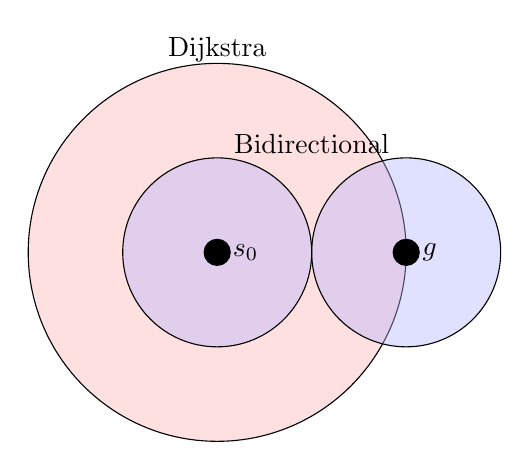
\begin{tikzpicture}[scale=0.6]
    \pgfmathsetmacro{\x}{2}
% forward search
\draw[fill=red!30, fill opacity=0.4] (0, 0) circle (2*\x);

% bidirectional search
\draw[fill=blue!30, fill opacity=0.4] (0, 0) circle (1*\x);
\draw[fill=blue!30, fill opacity=0.4] (2*\x, 0) circle (1*\x);


\node[draw,circle,fill=black] (a) at (0,0) {};
\node (aa) at (0+0.6, 0) {$s_0$};

\node[draw,circle,fill=black] (b) at (2*\x,0) {};
\node (bb) at (2*\x+0.5,0) {$g$};

\node (d) at (0, 2*\x+0.3) {Dijkstra};
\node (a) at (\x, 1*\x+0.3) {Bidirectional};

  \end{tikzpicture}
  }
  \caption{両方向探索}
  \label{fig:bidirectional}
\end{figure}



\section{外部メモリ探索 (External Search)}
\label{sec:external-search}


グラフ探索は重複検出のために今までに展開したノードをすべて保持しなければならない。
よって、保持できるノードの量によって解ける問題が決まってくる。
探索空間があまりに大きすぎると、ノードが多すぎてメモリに乗り切らないということが起きる。

\define{外部メモリ探索}{External Search}{がいぶメモリたんさく}は外部記憶、HDDやSDDを用いることでこの問題を解決する \cite{chiang1995external}。
すなわち、オープンリストとクローズドリストの一部を外部記憶に保持し、必要に応じて参照しメモリに持ってくる、ということをする。
外部メモリ探索のミソは、外部記憶へのアクセス回数をどのように減らすかにある。
表\ref{tbl:latency}は一般的なコンピュータのキャッシュ・メモリ・ハードディスクへのアクセスレイテンシーを比較した表である\footnote{表は\url{(https://gist.github.com/jboner/2841832)}より。}。メモリから1MB{\it 逐次に}読みだすオペレーションは250,000 nanosecかかるが、ハードディスクからの読出しは20,000,000 nanosecもかかる。更にハードディスクにランダムアクセスする場合(Disk seek)は8,000,000 nanosecもかかる。
よって、HDDは工夫して使わなければ実行時間が非常に遅くなってしまう。%\footnote{似たような理由で、HDDを用いないRAMベースの探索を効率化するためにはキャッシュ効率を工夫しなければならない。詳しくは\cite{burns2012implementing}を参照されたい。}。

\begin{table}
\centering
\caption{一般的なハードウェアのアクセス速度。メモリへのアクセス速度に対して外部記憶のアクセスは遅い。加えて、ランダムアクセスはseekの時間がかかるためさらに遅くなる。 }
\label{tbl:latency}
\begin{tabular}{|l|r|}
		   & nano sec \\ \hline
	命令実行 & 1 \\
	L1キャッシュからFetch & 0.5 \\
	分枝予測ミス 		& 5 \\
	L2キャッシュからFetch & 7 \\
	mutexロック・アンロック			& 25 \\
	メインメモリからFetch  	& 100 \\
	SSDから4KBをランダムにRead         & 150,000 \\
	メモリから1MBの連続した領域をRead & 250,000 \\
	ディスクから新しい領域をFetch & 8,000,000 \\
	SSDから1MBの連続した領域をRead		& 1,000,000 \\
	ディスクから1MBの連続した領域をRead 	& 20,000,000 \\
	
\end{tabular}
\end{table}

\subsection{外部メモリ 幅優先探索 (External BrFS)}
\label{sec:external-brfs}

一般に外部メモリが効率的であるためには問題に何らかの制約が必要になる。
例えばアルゴリズム\ref{alg:external-brfs}にある\define{外部メモリ幅優先探索}{external breadth-first search}{がいぶメモリはばゆうせんたんさく} (External BrFS)はグラフが無向グラフの時にしかうまくいかない \cite{mehlhorn2002external}。

\begin{figure}
  \centering
  \scalebox{0.75}{
  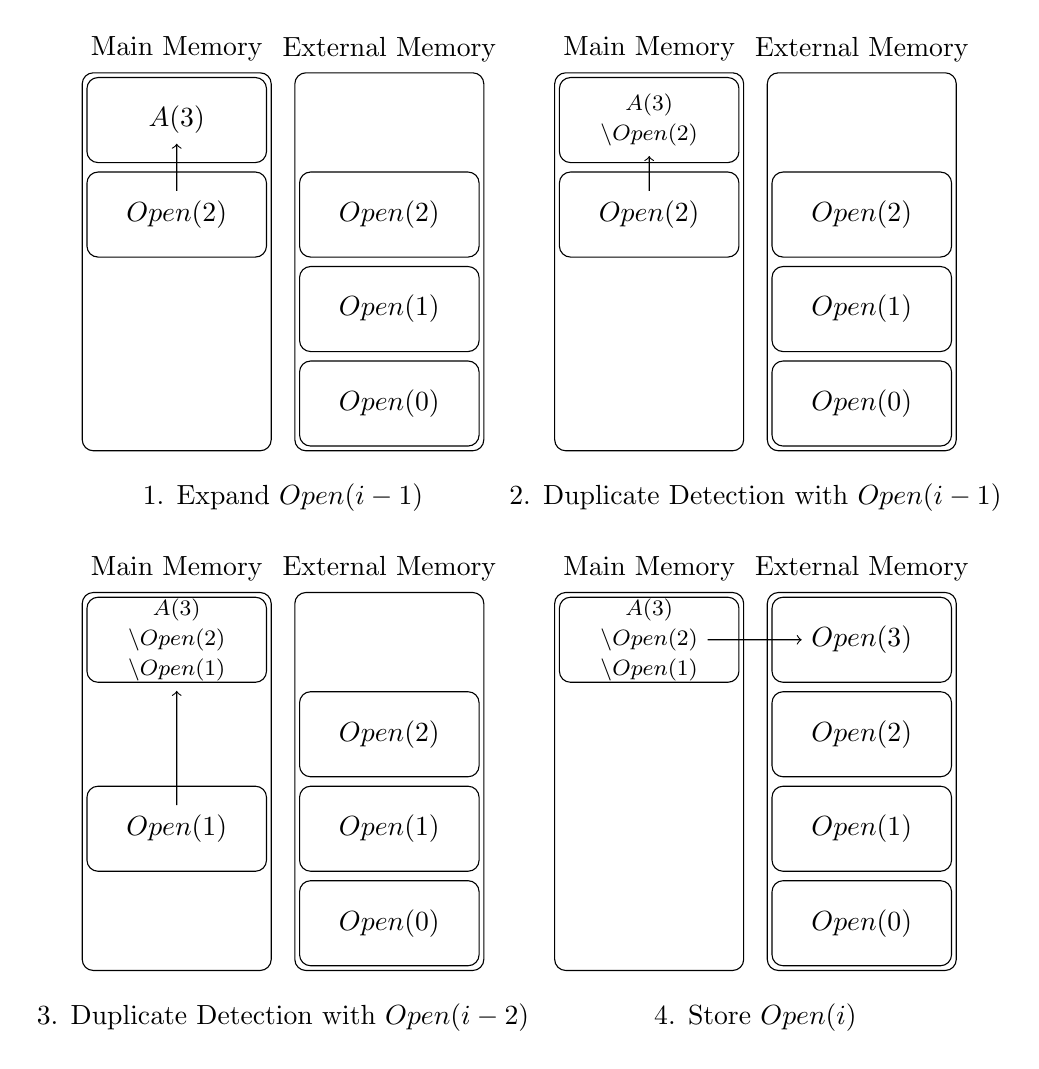
\begin{tikzpicture}[scale=0.6]
    \pgfmathsetmacro{\phi}{0.1}
\pgfmathsetmacro{\sp}{4.5}


%%%%%%%%%%%%%%%%%%%%%%%%
% State 1
%%%%%%%%%%%%%%%%%%%%%%%%

\pgfmathsetmacro{\bs}{0}
\pgfmathsetmacro{\bsy}{0}

% Memory
\draw[rounded corners] (\bs+0,0) rectangle (\bs+4, 8); 

% External disk
\draw[rounded corners] (\bs+\sp,0) rectangle (\bs+\sp+4, 8); 

\foreach \x in {0, 1, 2} {
  \draw[rounded corners] (\bs+\sp+\phi,\x*2+\phi) rectangle (\bs+\sp+4-\phi, \x*2+2-\phi);
  \node (\x) at (\bs+\sp+2,\x*2+1) {$Open(\x)$};
}

\draw[rounded corners] (\bs+\phi,2*2+\phi) rectangle (\bs+4-\phi, 2*2+2-\phi);
\node (mem2) at (\bs+2,2*2+1) {$Open(2)$};

\draw[rounded corners] (\bs+\phi,2*2+2+\phi) rectangle (\bs+4-\phi, 2*2+2+2-\phi);
\node (a2) at (\bs+2,2*2+2+1) {$A(3)$};
\draw[->] (mem2) -- (a2);

\node at ({\bs + (\sp + 4) / 2}, -1) {1. Expand $Open(i-1)$};

\node at ({\bs + 2}, \bsy+8.5) {Main Memory};
\node at ({\bs + \sp + 2}, \bsy+8.5) {External Memory};

%%%%%%%%%%%%%%%%%%%%%%%%
% State 2
%%%%%%%%%%%%%%%%%%%%%%%%

\pgfmathsetmacro{\bs}{10}
\pgfmathsetmacro{\bsy}{0}

% Memory
\draw[rounded corners] (\bs+0,0) rectangle (\bs+4, 8); 

% External disk
\draw[rounded corners] (\bs+\sp,0) rectangle (\bs+\sp+4, 8); 

\foreach \x in {0, 1, 2} {
  \draw[rounded corners] (\bs+\sp+\phi,\x*2+\phi) rectangle (\bs+\sp+4-\phi, \x*2+2-\phi);
  \node (\x) at (\bs+\sp+2,\x*2+1) {$Open(\x)$};
}

\draw[rounded corners] (\bs+\phi,2*2+\phi) rectangle (\bs+4-\phi, 2*2+2-\phi);
\node (mem2) at (\bs+2,2*2+1) {$Open(2)$};

\draw[rounded corners] (\bs+\phi,2*2+2+\phi) rectangle (\bs+4-\phi, 2*2+2+2-\phi);
\node[align=center,font=\footnotesize] (a2) at (\bs+2,2*2+2+1) {$A(3)$\\$\setminus Open(2)$};
\draw[->] (mem2) -- (a2);

\node at ({\bs + (\sp + 4) / 2}, -1) {2. Duplicate Detection with $Open(i-1)$};

\node at ({\bs + 2}, \bsy+8.5) {Main Memory};
\node at ({\bs + \sp + 2}, \bsy+8.5) {External Memory};


%%%%%%%%%%%%%%%%%%%%%%%%
% State 3
%%%%%%%%%%%%%%%%%%%%%%%%

\pgfmathsetmacro{\bs}{0}
\pgfmathsetmacro{\bsy}{-11}

% Memory
\draw[rounded corners] (\bs+0,\bsy+0) rectangle (\bs+4, \bsy+8); 

% External disk
\draw[rounded corners] (\bs+\sp,\bsy+0) rectangle (\bs+\sp+4, \bsy+8); 

\foreach \x in {0, 1, 2} {
  \draw[rounded corners] (\bs+\sp+\phi,\bsy+\x*2+\phi) rectangle (\bs+\sp+4-\phi, \bsy+\x*2+2-\phi);
  \node (\x) at (\bs+\sp+2,\bsy+\x*2+1) {$Open(\x)$};
}

\draw[rounded corners] (\bs+\phi,\bsy+2*1+\phi) rectangle (\bs+4-\phi, \bsy+2*1+2-\phi);
\node (mem1) at (\bs+2,\bsy+2*1+1) {$Open(1)$};

\draw[rounded corners] (\bs+\phi,\bsy+2*2+2+\phi) rectangle (\bs+4-\phi, \bsy+2*2+2+2-\phi);
\node[align=center,font=\footnotesize] (a2) at (\bs+2,\bsy+2*2+2+1) {$A(3)$\\$\setminus Open(2)$\\$\setminus Open(1)$};
\draw[->] (mem1) -- (a2);

\node at ({\bs + (\sp + 4) / 2}, \bsy-1) {3. Duplicate Detection with $Open(i-2)$};

\node at ({\bs + 2}, \bsy+8.5) {Main Memory};
\node at ({\bs + \sp + 2}, \bsy+8.5) {External Memory};



%%%%%%%%%%%%%%%%%%%%%%%%
% State 4
%%%%%%%%%%%%%%%%%%%%%%%%

\pgfmathsetmacro{\bs}{10}
\pgfmathsetmacro{\bsy}{-11}

% Memory
\draw[rounded corners] (\bs+0,\bsy+0) rectangle (\bs+4, \bsy+8); 

% External disk
\draw[rounded corners] (\bs+\sp,\bsy+0) rectangle (\bs+\sp+4, \bsy+8); 

\foreach \x in {0, 1, 2, 3} {
  \draw[rounded corners] (\bs+\sp+\phi,\bsy+\x*2+\phi) rectangle (\bs+\sp+4-\phi, \bsy+\x*2+2-\phi);
  \node (\x) at (\bs+\sp+2,\bsy+\x*2+1) {$Open(\x)$};
}

\draw[rounded corners] (\bs+\phi,\bsy+2*2+2+\phi) rectangle (\bs+4-\phi, \bsy+2*2+2+2-\phi);
\node[align=center,font=\footnotesize] (a2) at (\bs+2,\bsy+2*2+2+1) {$A(3)$\\$\setminus Open(2)$\\$\setminus Open(1)$};

\draw[->] (a2) -- (3);

\node at ({\bs + (\sp + 4) / 2}, \bsy-1) {4. Store $Open(i)$};

\node at ({\bs + 2}, \bsy+8.5) {Main Memory};
\node at ({\bs + \sp + 2}, \bsy+8.5) {External Memory};

  \end{tikzpicture}
  }
  \caption{外部メモリ幅優先探索の操作}
  \label{fig:external-brfs}
\end{figure}

\begin{algorithm}
\caption{外部メモリ幅優先探索 (External Breadth-first search)}
\label{alg:external-brfs}
	\Input{非明示的状態空間グラフ $(s, Goal, Expand, w)$}
	\Output{$s$からゴール状態$t \in T$への経路、経路が存在しなければ$\emptyset$}
	$Open(-1) \leftarrow \emptyset$\;
	$Open(0) \leftarrow \{s\}$\;
	$i \leftarrow 1$\;
	\While {$Open(i-1) \neq \emptyset$}{
		\If {$\exists (s \in Open(i-1)) Goal(s)$} {
			\Return $Path(s)$\;
		}
                
		$A(i) \leftarrow {u | u \in Expand(u'), u' \in Open(i-1)}$\;
                \For {each $s \in A(i)$} {
                  $parent(s) \leftarrow u$ s.t. $s \in Expand(u)$\;
                }
		$Open(i) \leftarrow A(i) \setminus (Open(i-1)\cup Open(i-2))$\;
		$i \leftarrow i + 1$\;
	}
	\Return $\emptyset$\;
\end{algorithm}

外部メモリ幅優先探索は深さ$i$のノードを$Open(i)$に保持する (図\ref{fig:external-brfs})。
$Open(i)$にあるノードを全て展開し、生成されたノードを$A(i)$に保存する。
$A(i)$にあるノードから$Open(i-1), Open(i-2)$と重複したノードを取り除き、残ったノードを$Open(i+1)$に入れる。
このような操作をすることによって、外部メモリ幅優先探索は深さ$i$のノードを展開するときは$Open(i)$のみをメインメモリに保持し、他の展開済みノードはすべて外部メモリに置くことができる。

グラフが無向グラフである場合、状態$s$と同じ状態は深さ$d(s)-2, d(s)-1, d(s)$にしか現れない。
よって深さ$i$のノードの集合$A(i)$は深さ$i-1, i-2$で発見されたノードとだけ重複検出をすれば十分である。
そのためオープンリストの全ノードではなく、$Open(i-1), Open(i-2)$のみを外部メモリから読み込んでくればよい。

もしグラフが有向グラフである場合、$Open(0), Open(1), ..., Open(i-1)$まですべてと重複検出を行う必要があり、その場合外部メモリに何度もアクセスしなければならない。


\section{シンボリック探索 (Symbolic Search)}
\label{sec:symbolic-search}
\define{二分決定グラフ}{Binary Decision Diagram}{にぶんけっていグラフ} (BDD)は二分木によってブーリアンの配列からブーリアンへの関数$(x_0,x_1,...,x_n) \rightarrow \{0, 1\}$を効率良く表すグラフ構造である \cite{akers1978binary,bryant1992symbolic}。
\define{シンボリック探索}{symbolic search}{シンボリックたんさく}はBDDを使って状態の集合、アクションの集合を表し、BDD同士の演算によって状態の集合を一気に同時に展開していく手法である \cite{edelkamp1998obdds,Edelkamp99deterministicstate}。
A*探索がノードを一つずつ展開していき、一つずつ生成していく手間と比較して非常に効率的に演算が出来るポテンシャルを秘めている。
また、オープン・クローズドリストをBDDで表せられるため、メモリ消費量が少なくなる場合がある。
2014年のInternational Planning CompetitionのSequential Optimal部門(最適解を見つけるパフォーマンスを競う部門)の一位から三位までをシンボリック探索が総なめした \cite{vallati20152014}。


\subsection{特徴表現 (Symbolic Representation)}
\label{sec:symbolic-representation}



\begin{figure}
  \centering
  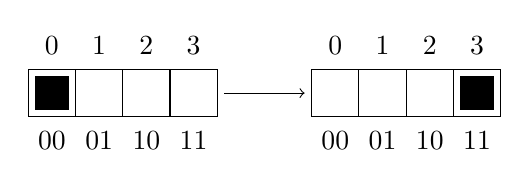
\begin{tikzpicture}[scale=0.6]
    
\pgfmathsetmacro{\phi}{0.15}

\foreach \base in {0, 6} {
  \draw (\base+0,0) grid (\base+4, 1);
  
  \foreach \x in {0, 1, 2, 3} {
    \node at (\base+\x+0.5, 1+0.5) {\x};  
  }

  \node at (\base+0+0.5, -1+0.5) {00};
  \node at (\base+1+0.5, -1+0.5) {01};
  \node at (\base+2+0.5, -1+0.5) {10};
  \node at (\base+3+0.5, -1+0.5) {11};

}

\draw[fill=black] (0+\phi,0+\phi) rectangle (1-\phi,1-\phi);

\draw[fill=black] (6+3+\phi,0+\phi) rectangle (6+4-\phi,1-\phi);

\draw[->] (4+\phi, 0.5) -- (6-\phi, 0.5);

  \end{tikzpicture}
\caption{特徴表現の例}
\label{fig:sliding-token}
\end{figure}


説明のために非常なシンプルなスライディングタイルパズルを考える(図\ref{fig:sliding-token})。
初期状態でタイルは位置0にあり、タイルを右か左に動かすことが出来る。タイルを位置3に動かせばゴールである。
この問題では状態は4通り$(S = \{0,1,2,3\})$しかないが、可能な状態の集合は$2^4$通りある $(2^S = \emptyset, \{0\}, \{1\}, \{2\}, \{3\}, \{0, 1\}, ..., \{0, 1, 2, 3\})$。
オープン・クローズドリストが保持する状態の集合はこのべき集合の要素である ($Open, Closed \in 2^S$)。

\define{特徴表現}{symbolic representation}{とくちょうひょうげん}はこの状態の集合を効率よく表現するための手法である。
状態の集合$O \in 2^S$に対して、ある状態$s$が$O$に含まれているかを返す関数$\phi_{O}: 2^S \rightarrow \{0, 1\}$を\define{特徴関数}{characteristic function}{とくちょうかんすう}と呼ぶ。

\begin{table}
\centering
\caption{特徴関数の例}
\label{tbl:sliding-token}
\begin{tabular}{c|c|c|c}
	状態 & コメント & ブーリアン表現 & 特徴関数 \\ \hline
	0		& 初期状態	& 00				& $\lnot x_0 \lnot x_1$ \\	
	1		& -			& 01				& $\lnot x_0  x_1$ \\	
	2		& -			& 10				& $x_0 \lnot x_1$ \\	
	3		& ゴール状態	& 11				& $x_0 x_1$ \\	
\end{tabular}
\end{table}

$\phi_O$は$O$に含まれる状態を全て明に保持すれば表現することが出来るが、もっと簡潔に表現することもできる。
まず、4通りの状態を2つのブーリアン変数 $s = (x_0, x_1)$で表すと$S = \{00, 01, 10, 11\}$になる。この表現を用いると、例えば$O = \{0\}$とすると、$\phi_{O}(x) = \lnot x_0 \lnot x_1$と表すことが出来る。$O = \{0, 1\}$ならば$\phi_{O}(x) = \lnot x_0$となる。

% 面白いことに、1つの状態のみを含む状態集合$S' = \{0\}$を表す特徴関数よりも要素2つの$S$を表す特徴関数の方が表現がコンパクトになる。
% このように、特徴表現は明示的に列挙するよりも状態の集合をコンパクトに表現出来る場合がある。

アクションによる状態遷移も特徴関数$Trans: S \times S \rightarrow \{0, 1\}$によって定義される。アクション$a \in A$によって状態$x$から$x'$に遷移するならば、$Trans_a(x,x')$は真を返す(かつその時のみ)。
アクション集合$A$による遷移は$Trans(x,x')$によって表現され、$Trans(x,x')$は$Trans_a(x,x')$が真となる$a \in A$が存在する場合に真を返す(かつその時のみ)。

図\ref{fig:sliding-token}の問題で可能なアクションは$(00) \rightarrow (01), (01) \rightarrow (00), (01) \rightarrow (10), (10) \rightarrow (01), (10) \rightarrow (11), (11) \rightarrow (10)$の6つである。これらを表す遷移関数は

\begin{equation}
\begin{split}
	Trans(x,x') &= (\lnot x_0 \lnot x_1 \lnot x'_0 x'_1) \\
		&\lor (\lnot x_0 x_1 \lnot x'_0 \lnot x'_1) \\
		&\lor (\lnot x_0 x_1 x'_0 \lnot x'_1) \\
		&\lor (x_0 \lnot x_1 \lnot x'_0 x'_1) \\
		&\lor (x_0 \lnot x_1 x'_0 x'_1) \\
		&\lor (x_0 x_1 x'_0 \lnot x'_1)
\end{split}
\end{equation}

となる。
アクションのコストがある場合は$Trans(w, x, x')$として表現され、$Trans(x,x')$は$Trans_a(x,x')$が真となる$a \in A$が存在し、かつそのアクションのコストが$w$である場合に真を返す(かつその時のみ)。


\subsection{二分決定グラフ (Binary Decision Diagram)}
\label{sec:binary-decision-diagram}

状態の集合や遷移関数はブーリアンによる特徴関数によって表すことができる。
この特徴関数は\define{二分決定グラフ}{binary decision diagram}{にぶんけっていグラフ} (BDD)というデータ構造によってコンパクトに保持しつつさまざまな集合演算を行うことができる。

\ddef{二分決定グラフ、BDD}{
BDDはループのない有向グラフであり、ノードとエッジはラベルが付いている。単一の根ノードと2つのシンクがあり、シンクのラベルは1と0である。sink以外のノードのラベルは変数$x_i (i \in \{1,...,n\})$であり、エッジのラベルは1か0である。
}

\begin{figure}
  \centering
  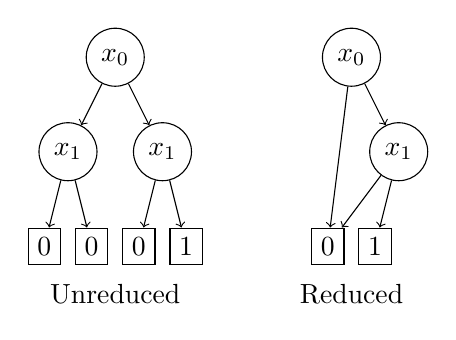
\begin{tikzpicture}[scale=0.6]
    % Unreduced
\node[circle,draw] (00) at (0, 4) {$x_0$};

\node[circle,draw] (10) at (-1, 2) {$x_1$};
\node[circle,draw] (11) at (1, 2) {$x_1$};

\node[rectangle,draw] (20) at (-1-0.5, 0) {$0$};
\node[rectangle,draw] (21) at (-1+0.5, 0) {$0$};
\node[rectangle,draw] (22) at ( 1-0.5, 0) {$0$};
\node[rectangle,draw] (23) at ( 1+0.5, 0) {$1$};

\draw[->] (00) -- (10);
\draw[->] (00) -- (11);

\draw[->] (10) -- (20);
\draw[->] (10) -- (21);
\draw[->] (11) -- (22);
\draw[->] (11) -- (23);

\node at (0, -1) {Unreduced};

% Reduced
\pgfmathsetmacro{\base}{5}
\node[circle,draw] (00) at (\base+0, 4) {$x_0$};

\node[circle,draw] (11) at (\base+1, 2) {$x_1$};

\node[rectangle,draw] (22) at (\base-0.5, 0) {$0$};
\node[rectangle,draw] (23) at (\base+ 0.5, 0) {$1$};

\draw[->] (00) -- (22);
\draw[->] (00) -- (11);

\draw[->] (11) -- (22);
\draw[->] (11) -- (23);

\node at (\base+0, -1) {Reduced};

  \end{tikzpicture}
  \caption{$x_0 x_1$を表す決定木 (左)とBDD (右)}
  \label{fig:bdd}
\end{figure}

BDDは決定木と同様な処理によって入力$x$に対して$\{1, 0\}$を返す。
すなわち、根ノードから始まり、ノードのラベル$x_i$に対して、入力$x$の$x_i$が1であればラベル1が付いたエッジをたどり、0であればラベル0をたどる。これを繰り返し、シンクにたどり着いたらシンクのラベルの値を返す。
決定木と異なりBDDは木ではなく、途中で合流などがあるため、決定木よりも空間効率が良い場合が多い (図\ref{fig:bdd})。
BDDは集合演算によってたくさんの状態に対して同時に展開・重複検知を行い、探索を進めることができる。



\subsection{特徴関数による状態空間の探索}

状態空間の探索は特徴関数の演算によって表現することが出来、その演算はBDDの演算によって実装することが出来る。

ある状態集合$S$に対して、$s \in S$となる$s$の次状態の集合を$S$の{\it image}と呼ぶ。
$S$のimageは以下の特徴関数によって表すことが出来る。

\begin{equation}
	Image_S(x') = \exists x (Trans(x,x') \land \phi_S(x))
\end{equation}

これを使ってグラフ探索アルゴリズムを実装することが出来る。
例えば$Image_{Open}(x')$はオープンリストにあるノードを全て展開して生成されるノードの集合になる。
重複検出にはこの中から$Closed(x)$に入っていないノードを取り出せばよい ($Image_{Open}(x) \land \lnot Closed(x)$)。

\subsubsection{BDD-幅優先木探索}

imageを繰り返し求めていくことで幅優先木探索は簡単に実装することが出来る。
まず、初期状態$s_0$だけによる集合$S_0 = \{s_0\}$を考える。これに対して$\phi_{S_{i}}$は集合$S_i$を表す特徴関数だとする。これを用いることで次状態集合を次々と求めることが出来る:

\begin{equation}
	\phi_{S_i}(x') = \exists x (\phi_{S_{i-1}}(x) \land Trans(x,x'))
\end{equation}

簡単に言えば、状態$x'$は、もし親状態$x$が$S_{i-1}$に含まれていれば、$S_i$に含まれる。
探索を停止するためには探索した状態にゴール状態が含まれているかをテストしなければならない。
ゴールテストも特徴関数を用いて表すことが出来る。
ゴール状態集合$T$を表す特徴関数を$\phi_T$とすると、$\phi_{S_i}(x') \land \phi_T \neq false$であれば$S_i$はゴール状態を含む。

アルゴリズム\ref{alg:symbolic-brfs-tree}はBDD-幅優先木探索である。
imageの計算とゴールテストによって実装することが出来る。


\begin{algorithm}
\caption{BDD幅優先木探索 (BDD-Breadth-first Tree Search)}
\label{alg:bdd-brfs-tree}
	\Input{非明示的状態空間グラフ $P = (s, Goal, Expand, w)$、前状態 $s'$}
	\Output{$s$からゴール状態$t \in T$への経路、経路が存在しなければ$\emptyset$}
	$S_0 \leftarrow \{s\}$\;
	\For {$i \leftarrow 1, 2, ...$} {
		$\phi_{S_i}(x) \leftarrow \exists x (\phi_{S_{i-1}}(x) \land Trans(x,x'))[x'/x]$\;
		\If {$\phi_{S_i}(x) \land \phi_T \neq false$} {
			\Return $Construct(\phi_{S_i} \land \phi_T(x), i)$\;
		}
	}
%	\Return No solution found
\end{algorithm}


$Construct$関数はゴールに至るための経路を計算する関数である。
$\phi_{S_i} \land \phi_T(x)$によってゴール状態、解経路における$i$ステップ目の状態($s_i$)が得られる。次に$Trans(\phi_{S_{i-1}}, s_i)$によって$i-1$ステップ目の状態$s_{i-1}$が得られ、$Trans_a$を見ていくことで$i-1$ステップ目のアクションが得られる。これを繰り返すことによって元の解経路を復元することが出来る。ゴール状態は一つ取り出せば十分であるため、$Construct$の計算時間は大きくはない。

BDD-幅優先木探索は幅優先探索と同様、解の経路長が最短であることを保証する。


\subsubsection{BDD-幅優先グラフ探索}

重複検出を行う場合はクローズドリストに展開済みノードを保存する必要がある。
この展開済みノードも特徴関数及びBDDで表すことが出来る。
アルゴリズム\ref{alg:bdd-brfs}はBDD-幅優先探索のコードである。
アルゴリズム\ref{alg:bdd-brfs-tree}と異なり特徴関数$Closed$を用いて重複検出を行っている。

\begin{algorithm}
\caption{BDD幅優先探索 (BDD Breadth-first search)}
\label{alg:bdd-brfs}
	\Input{非明示的状態空間グラフ $P = (s, Goal, Expand, w)$、前状態 $s'$}
	\Output{$s$からゴール状態$t \in T$への経路、経路が存在しなければ$\emptyset$}
	$S_0 \leftarrow \{s_0\}$\;
	$Closed \leftarrow \{s_0\}$\;
	\For {$i \leftarrow 1, 2,...$} {
		$Succ(x) \leftarrow \exists x (\phi_{S_{i-1}}(x) \land Trans(x,x'))[x'/x]$\;
		$\phi_{S_i}(x) \leftarrow Succ(x) \land \lnot Closed(x)$\;
		$Closed(x) \leftarrow Closed(x) \lor Succ(x)$\;
		\If {$\phi_{S_i}(x') \land \phi_T \neq false$} {
			\Return $Construct(\phi_{S_i} \land \phi_T(x), i)$\;
		}
	}
%	\Return No solution found
\end{algorithm}

% TODO: BDD-最適コスト探索
% \subsubsection{BDD-最適コスト探索}

% Not for now
%\subsection{Symbolic Tree Search}
%\subsection{Symbolic Blind Search}
%\subsection{Symbolic Heuristic Search}

% \subsection{関連文献}




\section{新奇性に基づく枝刈り (Novelty-based Pruning)}
\label{sec:novelty-based-pruning}

状態空間を広く探索することは局所最適やデッドエンドに陥らないためには必要である。
より\define{新奇性}{novelty}{しんきせい}のある状態を優先して探索することによって広く状態空間が探索できると考えられる。
状態空間が非常に大きい場合は、よりアグレッシブに、すでに生成された状態と似たような状態を枝刈りしていく方法がある。


%新奇性は似たような状態というのが定義しやすいドメインにおいて有効である。


\subsection{状態の新奇性 (Novelty)}
\label{sec:novelty}

状態に対して新奇性を定義する試みは古くから人工知能研究にある\cite{lehman2008exploiting}。
なので新奇性の定義も様々であるが、本書では\cite{geffner2015}の定義に従い、新奇性を以下のように定義する。

\ddef{新規性、Novelty}{
$m$個の特徴関数の集合$h_1,h_2,....,h_m$に対して新たに生成された状態$s$の新奇性$w(s)$は$n$であるとは、
$n$個の特徴関数によるタプル$\{h_{i_1},h_{i_2},..,h_{i_n}\}$が存在し、
$h_{i_1}(s) = h_{i_1}(s')$, $h_{i_2}(s) = h_{i_2}(s')$,...,$h_{i_n}(s) = h_{i_n}(s')$を満たす生成済みの状態$s'$が存在せず、
かつ、この条件を満たすそれよりも小さいタプルが存在しない。
}

特徴関数は単純に状態変数の値を返す関数を使うことができる \cite{geffner2015, lipovetzky2015a}。
つまり状態$s = \{v_1, v_2,...,v_m\}$に対して特徴関数は$h_i = v_i$とする。
この場合、$w(s) = m$であれば状態変数がすべて同じノードがすでに生成済みであるということなので、$s$は重複したノードである。
このため枝刈りのために新奇性を定義する場合はこれが便利である。

% TODO: もっとわかりやすい例?
% 例えばマルバツゲームの新奇性を考える。
% 特徴関数$h_i$は$i$の位置にあるマーク(空、マル、バツ)を返す。
% 初期状態$s_0$の新奇性は生成済み状態が存在しないので1である。

% \begin{figure}
% TODO: マルバツゲームの図
% \caption{マルバツゲームにおける新奇性の例}
% \end{figure}

\subsection{幅制限探索 (Width-Based Search)}
\label{sec:width-based-search}

\define{幅制限探索}{width-based search}{はばせいげんたんさく}は状態の新奇性に基づいてノードを枝刈りする手法である \cite{lipovetzkyg12}。
新奇性によってノードを枝刈りするので、解が存在しても発見される保証はない (完全性を満たさない)。

\begin{algorithm}[tbh]
\caption{幅制限探索 (Width-based search)}
\label{alg:width-based-search}
	\Input{非明示的状態空間グラフ $(s, Goal, Expand, w)$、特徴関数 $h_0, h_1,..., h_{m-1}$、幅$i$}
	\Output{$s$からゴール状態$t \in T$への経路、経路が存在しなければ$\emptyset$}
	$Closed \leftarrow \emptyset$, $Open \leftarrow \{s\}$\;
	\While{$Open \neq \emptyset$} {
                $u \leftarrow \argmin_{u' \in Open} f(u')$ \;
		$Open \leftarrow Open \setminus \{u\} $\;
		\If {$Goal(u)$} {
			\Return $Path(u)$\;
		}
		\For {each $v \in Expand(u)$} {
                  $H(v) \leftarrow \{j | j \in \{0, 1, ..., m-1\}, h_j(v) = 1\}$\;
                  $H \leftarrow \{j | j \in \{0, 1, ..., m-1\}, h_j(v) \in Closed\}$\;
                  \If{$|H \setminus Closed| \geq i$} {
                    $Open \leftarrow Open \cup \{v\}$\;
                    $parent(v) \leftarrow u$\;
                  }
                  \For {each $h \in H(v) \setminus Closed$} {
                    $Closed \leftarrow Closed \cup \{h\}$\;
                  }
		}
 	}
	\Return $\emptyset$\;
\end{algorithm}

IW($i$)は新奇性が$i$よりも大きい状態を枝刈りする探索である。
新奇性に基づく枝刈りには2つのメリットがある。
一つは状態空間が著しく小さくなる。
もう一つは幅を制限することで生成済みノードをクローズドリストにすべて保存する必要がなくなる。
その代わり保存しなければならない情報は、生成済みの特徴のタプルのうち大きさが$i$以下のものの集合である。
これがないと新奇性を計算することができない。
IWにおけるクローズドリストは過去に真であったことのある特徴の集合である。
状態$s$において真である特徴の集合を$H$としたとき、$H$に存在し$Closed$に存在しない特徴の数が$i$以上かどうかを確認し、$i$以上であればそのノードを生成する。そうでなければ枝刈りを行う。

幅$i$を大きくするほど発見できる解のクオリティが上がりやすいが、一方探索空間は$i$に対して指数的に大きくなっていく。
このトレードオフを調整しやすくするために新奇性の定義域を有理数に拡張した幅制限探索が提案されている\cite{geffner2015}。


\subsection{反復幅制限探索 (Iterative Width Search)}
\label{sec:iterative-width-search}

\define{反復幅制限探索}{iterative width search}{はんぷくはばせいげんたんさく}は幅制限探索を幅を大きくしながら解を発見するまで繰り返すアルゴリズムである \cite{lipovetzkyg12}。
IW($i$)は幅$i$が大きくなるほど解のクオリティが良くなるが、より大きな状態空間を探索することになる。
反復幅制限探索は小さい幅からはじめ、解が見つからない・良い解でなければ幅を大きくして再度探索を行う手法である。
いずれ幅の大きさが特徴の数と同じまでになるので、反復幅制限探索は解があればいずれ必ず発見する。

\begin{algorithm}
\caption{反復幅制限探索 (Iterative Width Search)}
$i \leftarrow 1$\;
$path \leftarrow \emptyset$\;
	\While {$path = \emptyset$} {
		$path \leftarrow IW(i)$\;
		$i \leftarrow i + 1$\;
	}
	\Return $path$
\end{algorithm}

\begin{comment}

\subsection{Best-First Width Search (最良優先幅制限探索)}
\label{sec:width-based-heuristic-search}

\cite{geffner2015}


\subsection{Novelty Heuristics (新奇性に基づくヒューリスティック)}
\label{sec:novelty-heuristics}

ここまでの議論では新奇性を枝刈りのために使った。
しかしノードを捨ててしまう枝刈りは解が存在する問題でも解を発見できなくなってしまうという問題がある。
新奇性を使ってノードを完全に捨ててしまうのではなく、新奇性に基づいてノードを展開する優先度を決めるというアプローチをとることができる \cite{geffner2015}。つまり新奇性をヒューリスティックに使うということである。
この方法ではノードは完全に捨てられることはないので解を捨ててしまう可能性はなくなる。

ここで注意しなければならないのは新奇性は生成済みノード集合に依存する値である。
つまり新奇性に基づくヒューリスティック関数は状態$s$の関数ではなく、状態とクローズドリストの関数となる。つまり、同じ状態のノードでもヒューリスティック値が異なる場合がある。

% TODO: read the paper
\end{comment}

% \subsection{関連文献}
% Best-First Width Search (最良優先幅制限探索) \cite{geffner2015}
% Novelty Heuristics (新奇性に基づくヒューリスティック) \cite{geffner2015}


\section{並列探索 (Parallel Search)}
\label{sec:parallel-search}

近年コンピュータ一台当たりのコア数は増加を続けており、コンピュータクラスタにも比較的容易にアクセスが出来るようになった。Amazon Web Serviceのようなクラウドの計算資源も普及し、将来的には並列化が当然になると考えられる。
並列化の成功例は枚挙にいとまないが、近年のディープラーニングはまさに効率的な並列計算アーキテクチャによって得られたブレイクスルーであるといえる。
%残念ながら、探索アルゴリズムの並列化は比較的難しいと考えられる。
%一般に並列アルゴリズムの効率は逐次実行部分と並列実行可能部分に分割される
%グラフ探索アルゴリズムを並列化するメリットの一つはもちろん実行速度の高速化である。
グラフ探索アルゴリズムの並列化に考えなければならないオーバーヘッドは様々であり、それらの重要性は問題、インスタンス、マシン、さまざまな状況に依存する。% 加えてハードウェアは刻々と変化を続けており、数年後にどのような環境がメジャーとなるのかはなかなか想像をすることが出来ないだろう。
% 本書ではCPUを用いた分散メモリ並列アルゴリズムとGPU一台を用いた並列アルゴリズムについて説明する。
CPU並列ではハッシュによってノードを各プロセスにアサインし、各プロセスはアサインされたノードのみを担当して探索を行うというフレームワークが有効である。
より詳細な議論は\ref{fukunaga2017survey}を参照されたい。

\subsection{並列化オーバーヘッド (Parallel Overheads)}
\label{sec:parallel-overheads}

理想的には$n$プロセスで並列化したら$n$倍速くなってほしい。
逐次アルゴリズムと比較して、プロセス数倍の高速化が得られることを\define{完全線形高速化}{perfect linear speedup}{かんぜんせんけいこうそくか}と呼ぶ。
しかしながら、殆どの場合完全線形高速化は得られない。
それは並列化にさいして様々なオーバーヘッドがかかるからである。
\cite{jinnai2017work}の記法に従うと、並列化オーバーヘッドは主に以下の3つに分けられる。

\ddef{通信オーバーヘッド、communication overhead}{
  プロセス間で情報交換を行うことにかかる時間を\define{通信オーバーヘッド}{communication overhead}{つうしんオーバーヘッド} (CO)と呼ぶ。
}

通信する情報は様々なものが考えられるが、オーバーヘッドとなるものはノードの生成回数に比例した回数通信を必要とするものである。
すなわち、ノードの生成回数$n$に対して$log(n)$回しか通信を行わない場合、その通信によるオーバーヘッドは無視出来るだろう。
ここではノードの生成回数に対するメッセージ送信の割合をCOと定義する:
\begin{equation}
	CO := \frac{\text{他プロセスへ送信されたメッセージの数}}{\text{生成されたノードの数}}.
\end{equation}
例えば、ハッシュなどによってプロセス間でノードの送受信を行いロードバランスを行う手法 (e.g. 後述するHDA*)の場合、通信するメッセージは主にノードである。この場合:

\begin{equation}
	CO := \frac{\text{他プロセスへ送信されたノードの数}}{\text{生成されたノードの数}}.
\end{equation}
となる。
COは通信にかかるディレイだけでなく、メッセージキューなどのデータ構造の操作も行わなければならないので、特にノードの展開速度が速いドメインにおいて重要なオーバーヘッドになる。一般に、プロセス数が多いほどCOは大きくなる。
%If nodes are assigned randomly to the threads, CO will be proportional to $1-\frac{1}{\#thread}$. 

\ddef{探索オーバーヘッド、Search Overhead}{
  並列化によって余分に増えた展開ノード数の割合を探索オーバーヘッドと呼ぶ。
}

一般に並列探索は逐次探索より多くのノードを展開することになる。
このとき、余分に展開したノードは逐次と比較して増えた仕事量だと言える。
本書では以下のように探索オーバーヘッドを定義する:

\begin{equation}
  SO := \frac{\text{並列探索で展開されるノード数}}{\text{逐次探索で展開されるノード数}} - 1.
\end{equation}

SOは\define{ロードバランス}{load balance}{ロードバランス} (LB)が悪い場合に生じることが多い。

\begin{equation}
LB := \frac{\text{各プロセスに割り当てられたノード数の最大値}}{\text{各プロセスに割り当てられたノード数の平均}}.
\end{equation}

ロードバランスが悪いと、ノードが集中しているスレッドがボトルネックとなり、他のスレッドはノードがなくなるか、あるいはより$f$値の大きい(有望でない)ノードを展開することになり、探索オーバーヘッドになる。

探索オーバーヘッドは実行時間だけでなく、空間オーバーヘッドでもある。ムダに探索をした分だけ、消費するメモリ量も多くなる。分散メモリ環境においてもコア当りのRAM量は大きくなるわけではないので、探索オーバーヘッドによるメモリ消費は問題となる。

\ddef{同期オーバーヘッド、Coordination Overhead} {
  他のスレッドの処理をアイドル状態で待たなければならない時間の割合を\define{同期オーバーヘッド}{coordination overhead}{どうきオーバーヘッド}と呼ぶ。
}

アルゴリズム自体が同期を必要としないものだとしても、メモリバスのコンテンションによって同期オーバーヘッドが生じることがある\cite{burnslrz10,kishimotofb13}.


これらのオーバーヘッドは独立ではなく、トレードオフの関係にある。
多くの場合、通信・同期オーバーヘッドと探索オーバーヘッドがトレードオフの関係にあたる。


\subsection{並列A* (Parallel A*)}

\define{並列A*}{parallel A*}{へいれつエースター} (PA*)はA*探索のシンプルな並列化である \cite{iranis86}。PA*は一つのオープンリスト・クローズドリストを全てのプロセスで共有してアクセスする。オープンリスト・クローズドリストには複数のプロセスが同時にアクセスできないようにロックがかけられる。
PA*の問題点はデータ構造を一つに集中させているため、分散メモリ環境の場合はアクセスに大きな通信オーバーヘッドが生じることである。
共有メモリ環境の場合でも、それぞれのプロセスは他のプロセスがデータ構造にアクセスしている間にはアクセスできないため、同期オーバーヘッドが生じる。この同期オーバーヘッドはプロセスの数が増えるほど問題になる。ロックフリーのデータ構造を使ってもこのオーバーヘッドは解消されない \cite{burnslrz10}。

\subsection{ハッシュ分配A* (Hash Distributed A*)}
\label{sec:hash-distributed-astar}

PA*の問題点はすべてのプロセスが共有された一つのデータ構造へアクセスしなければならない点である。このような手法を\define{集中型手法}{centralized approach}{しゅうちゅうがたしゅほう}と呼ぶ。
共有データ構造へのアクセスは計算のボトルネックとなり、スケーラビリティの限界点になってしまう。
そのため、A*の並列化には各プロセスが自分のオープンリスト・クローズドリストを持ち、アクセスを分散させる\define{分散型手法}{decentralized approach}{ぶんさんがたしゅほう}が有力である。
分散型手法はデータ構造へのアクセスが分散するため同期オーバーヘッドを解消される。一方、各プロセスがアクセスするデータ構造が異なるため、各プロセスの仕事量を均等に分配しずらいという\define{ロードバランシング}{load balancing}{ロードバランシング}の問題が生じる。各プロセスに対してどのようにして仕事を均等に分配するかが問題になる。

\define{ハッシュ分配A*}{Hash Distributed A*}{ハッシュぶんぱいエースター} (HDA*) \cite{kishimotofb13}はstate-of-the-artの並列A*探索アルゴリズムである。
HDA*の各プロセスはそれぞれローカルなオープンリスト、クローズドリストを保持する。ローカルとは、データ構造を保持するプロセスが独占してアクセスを行い、他のプロセスからはアクセスが不可能であるという意味である。
グローバルなハッシュ関数によって全ての状態は一意に定まる担当のプロセスが定められる。
各プロセス$T$の動作は以下を繰り返す (アルゴリズム\ref{alg:hdastar}):

\begin{enumerate}
	\item 
		プロセス$T$はメッセージキューを確認し、ノードが届いているかを確認する。届いているノードのうち重複でないものをオープンリストに加える(A*同様、クローズドリストに同じ状態が存在しないか、クローズドリストにある同じ状態のノードよりも$f$値が小さい場合に重複でない)。
	\item 
		オープンリストにあるノードのうち最もプライオリティ($f$値)の高いノードを展開する。生成されたそれぞれのノード$n$についてハッシュ値$H(n)$を計算し、ハッシュ値$H(n)$を担当するプロセスに非同期的に送信される。
\end{enumerate}


\begin{algorithm}
  \caption{Hash Distributed A*}
  \Input{非明示的状態空間グラフ $(s, Goal, Expand, w)$、ヒューリスティック関数$h$、ハッシュ関数 $H$}
  \Output{$s$からゴール状態$t \in T$への経路、経路が存在しなければ$\emptyset$}
  $Closed_p \leftarrow \emptyset$, $Open_p \leftarrow \emptyset$, $\mathit{Buffer}_p \leftarrow \emptyset$ for each thread $p$\;
  $Open_{H(s)} \leftarrow \{s\}$, $g(s) \leftarrow 0$\;
  $goal \leftarrow \emptyset$, $c' \leftarrow \infty$\;

  \For {each process $p$} {
  \While {{\bf not} $TerminateDetection()$} {
    \For {each $(v, g_v, p_v) \in \mathit{Buffer}_p$} {
      \If{$v \notin Closed$ {\bf or} $g_v < g(v)$} {
        $Open \leftarrow Open \cup \{v\}$\;
	$g(v) \leftarrow g_v$\;
        $parent(v) \leftarrow p_vv$\;
      }
      \If{$v \notin Closed$} {
        $Closed \leftarrow Closed \cup \{v\}$\;
      }
    }
    $\mathit{Buffer}_p \leftarrow \emptyset$\;
    \While {$Open_p \neq \emptyset$ {\bf and} $min_{s \in Open_p} f(s) < c'$} {
      $u \leftarrow \argmin_{u' \in Open} f(u')$ \;
      $Open \leftarrow Open \setminus \{u\} $\;

      \If {$Goal(u)$ {\bf and} $g(u) < c'$} {
        $goal \leftarrow u$\;
        $c' \leftarrow g(u)$\;        
      }

      \For {each $v \in Expand(u)$} {
        $g_v \leftarrow g(u) + w(u, v)$\;
        $\mathit{Buffer}_{H(v)} \leftarrow \mathit{Buffer}_{H(v)} \cup \{(v, g_v, u)\}$\;
      }
    }
  }
  \Return $Path(goal)$\;
  }
  \label{alg:hdastar}
\end{algorithm}

HDA*の重要な特徴は2つある。
まず、HDA*は非同期通信を行うため、同期オーバーヘッドが非常に小さい。
各プロセスがそれぞれローカルにオープン・クローズドリストを保持するため、これらのデータ構造へのアクセスにロックを必要としない。
次に、HDA*は手法が非常にシンプルであり、ハッシュ関数$Hash: S \rightarrow {1..P}$を必要とするだけである ($P$はプロセス数)。
%並列アルゴリズムにおいて手法がシンプルであることは非常に有用である。
しかしながらハッシュ関数は通信オーバーヘッドとロードバランスの両方を決定する為、その選択はパフォーマンスに非常に大きな影響を与える。

HDA*が提案された論文\cite{kishimotofb13}ではZobrist hashing \cite{zobrist:70}がハッシュ関数として用いられていた。
状態$s = (x_1,x_2,...,x_n)$に対してZobrist hashingのハッシュ値$Z(s)$は以下のように計算される:

\begin{equation}
\label{eq:zobrist}
 	Z(s) := R_{0}[x_{0}]\; xor\; R_{1}[x_{1}]\; xor\; \cdots\; xor\; R_{n}[x_{n}]%
\end{equation}

Zobrist hashingは初めにランダムテーブル$R$を初期化する\ref{alg:init-zobrist-hashing}。
これを用いてハッシュ値を計算する。

\begin{algorithm}
	\caption{Zobrist Hashing}
	\Input{$s = (x_0, x_1,...,x_n)$}
	$hash \leftarrow 0$\;
	\For {each $x_i \in s$} {
		$hash \leftarrow hash \; xor \; R[x_i]$\;
	}
	\Return $hash$\;
	\label{alg:zobrist-hashing}
\end{algorithm}

\begin{algorithm}
	\caption{Zobrist Hashingの初期化}
	\Input{$V = (dom(x_0),dom(x_1),...)$}
	\For {each $x_i$} {
		\For {each $t \in dom(x_i)$ } {
			$R_i[t] \leftarrow random()$\;
		}
	}
	\Return $R = (R_1, R_2,...,R_n)$
	\label{alg:init-zobrist-hashing}
\end{algorithm}

Zobrist hashingを使うメリットは2つある。
一つは計算が非常に速いことである、XOR命令はCPUの演算で最も速いものの一つである。かつ、状態の差分を参照することでハッシュ値を計算することが出来るので、アクション適用によって値が変化した変数の$R[x]$のみ参照すれば良い。
もうひとつは、状態が非常にバランスよく分配され、ロードバランスが良いことである。
一方、この手法の問題点は通信オーバーヘッドが大きくなってしまうことにある。
この問題を解決するためにState abstractionという手法が提案された\cite{burnslrz10}。
State abstractionは状態$s = (x_1,x_2,...,x_n)$に対して簡約化状態 (abstract state) $s' = (x_1',x_2',...,x_m'), \; where \; m < n, x_i' = x_j (1 \leq j \leq n)$. % TODO: clean up this.
State abstractionは簡約化状態からハッシュ値への関数の定義はされておらず、単純なlinear congrugent hashingが用いられていた。そのため、ロードバランスが悪かった。

Abstract Zobrist hashing (AZH)はZobrist hashingとAbstractionの良い点を組み合わせた手法である\cite{jinnai2016structured}。AZHはfeatureからabstract featureへのマッピングを行い、abstract featureをZobrist hashingへの入力とするという手法である:

\begin{equation}
\label{eq:abstract-zobrist}
 	Z(s) := R_{0}[A_0(x_{0})]\; xor\; R_{1}[A_1(x_{1})]\; xor\; \cdots\; xor\; R_{n}[A_n(x_{n})]%
\end{equation}

ここで関数$A$はfeatureからabstract featureへのマッピングであり、$R$はabstract featureに対して定義されている。
% Abstract featureを自動的に生成する手法は複数提案されており、最もシンプルなものはGreedy abstract feature generation \cite{jinnai2016automated}である。

HDA*のための分解関数の自動生成方法は\cite{jinnai2017work}にまとめられている。

% \subsection{関連文献}
% 並列深さ優先探索 \cite{kumar1988parallel}.
% Transposition Table Driven Work Distribution (TDS) \cite{}.
% Parallel Structured Duplicated Detection (PSDD) \cite{}.
% Parallel Best-NBlock First (PBNF) \cite{}.
% 
% 
% 一方、執筆時現在、GPUを用いたアルゴリズムはあまり研究が進んでいない。原因としては、既存のCPUを用いた探索アルゴリズムにはない様々な難しさがあるだろう。
% たとえば、GPUはスレッド当りのメモリ量が非常に少ない。A*探索はメモリが大きなボトルネックであり、メモリ量が少ないとそのまま解ける問題の大きさが制限されてしまう。この問題を解決する方法は提示されていない。
% もうひとつの難しさは、GPUは複数のスレッドが同じ命令を実行するSingle instruction multiple thread (SIMT)という計算モデルであることである。そのため、既知の有力なヒューリスティック関数をGPU環境において効率的に実装する方法が自明ではない。
% パターンデータベースなどのシンプルな命令によるヒューリスティックも考えることが出来るが、このようなヒューリスティックは今度はメモリを沢山消費するという問題点がある。
% 効率的なGPU並列化アルゴリズムの開発は大きな成果が期待されるブルーオーシャンであるといえる\footnote{個人の感想である}。
% もしCPU/GPUを利用した効率的なグラフ探索アルゴリズムが開発出来れば、非常に大きなインパクトになるかもしれない。


%  
% \section{モンテカルロ木探索 (Monte Carlo Tree Search)}
% \label{sec:mcts}
% 
% モンテカルロ木探索 (Monte Carlo Tree Search, MCTS)は非常に多様な問題で応用されている手法である。
% その長所はたくさんある。
% まず、MCTSは状態空間が非決定論的でも扱える。不完全情報でも扱える。
% 2人プレイヤーゲームなどにも使える。特に碁で使われている。Alpha Goでも使われた。
% 
% MCTSのエージェントは木データ構造を保持する。
% 木の根は初期状態(2人プレイヤーゲームなどでは現在の盤面を初期状態とする)である。
% MCTSは初期状態から木を辿り、木に新しいノードを追加する、というイテレーションを繰り返す。
% 一つのイテレーションは4つの処理のループからなる。
% 
% \begin{enumerate}
% \item Select a next node following a tree policy
% \item Add a new node to the tree
% \item Simulate following a default policy
% \item Back propagate
% \end{enumerate}
% 
% 
% 
% \begin{algorithm}
% \caption{Monte Carlo Planning(state)}
% \label{alg:mcts}
% 	\While {True} {
%     	search(state, 0)
%     }
%     \Return bestAction(state, 0)
% \end{algorithm}
% 
% \begin{algorithm}
% \caption{search(state, depth)}
% \label{alg:mcts-iter}
% 	\If {Terminal(state)} {
%     	\Return 0
%     }
%     \If {Leaf(state, d)} {
%     	\Return Evaluate(state)
%     }
%     action $\leftarrow$ selectAction(state, depth)\;
%     (nextstate, reward) $\leftarrow$ simulateAction(state, action)\;
%     q $\leftarrow$ reward + $\gamma$ search(nextstate, depth + 1)\;
%     UpdateValue(state, action, q, depth)
% \end{algorithm}
% 
% \subsection{UCT (UCB1 Applied to Tree)}
% \label{sec:uct}
% 
% MCTSのtree policyの選択は状態空間をどのように探索するかに大きな影響を与える。
% 最も広く使われているtree policyはUCB1による \cite{UCT 2006,survey論文}。
% 
% \begin{equation}
% 	UCB1(s, s') = \bar{X_{s'}} + 2 C_p \sqrt{\frac{2 \ln n(s)}{\ln n(s')}}
% \end{equation}
% 
% where $\bar{X_{s'}}$ is the average reward from visiting $s'$, $n(s), n(s')$ is a number of visits to state $s$, $s'$, respectively.
% UCB1を使うMCTSはUpper bound applied to tree (UCT)と呼ばれる。
% 
% \section{その他の派生アルゴリズム}
% ここで紹介した以外にもヒューリスティック探索の派生アルゴリズムはたくさんある。
% 
% \define{再帰的最良優先探索}{Recursive best-first search} (RBFS)はIDA*の拡張である \cite{RBFS}。
% RBFSはノードを最良優先の順で展開し、ヒューリスティック値をバックアップする。
% 余ったメモリを使ってノードの展開数を抑える拡張が提案されている (Memory-aware RBFS) \cite{MRBFS}。
% 
% %Depth-first iterative deepening
% Partial Expansion A* \cite{}。多重整列問題。
% 
% K-Best First Search
% 
% K-ビームサーチ
% Partial A*
% Partial IDA*
% MA*
% Frontier Search
% 
% 
% ポートフォリオ戦略
% どれか一つのアルゴリズムに絞らなくてもよい
% いろいろ試してみるのが有効なことが多い



% -*- coding: utf-8 -*-

\chapter{自動行動計画問題 (Automated Planning Problem)}
%\chapter{古典的プランニング問題 (Classical Planning Problem)}
\label{ch:classical-planning}

本書の冒頭でグラフ探索アルゴリズムが人工知能のための技術として研究されていると説明した。
人工知能とはさまざまな定義で使われる言葉であるが、グラフ探索は自動推論や自動行動計画のために使うことができるために研究されている。
この章では人工知能の一分野である\define{自動行動計画問題}{automated planning problem}{じどうこうどうけいかくもんだい}について説明する \cite{ghallab:04}。
自動行動計画は初期状態から命題集合で表される目的を達成するための{\bf プラン}を発見する問題である。
自動行動計画のためのモデルは様々提案されている。
最も基本となるモデルは古典的プランニング問題である \cite{fikes:71}。
古典的プランニングは完全情報\footnote{正確には完全情報ではなく、アクションの決定のために必要な情報がすべて得られると仮定される。例えば問題に全く関係ない冗長な変数が含まれ、その情報がエージェントに与えられない場合は完全情報ではないが、アクションの決定のためには不要な情報であれば古典的プランニング問題で扱うことができる。}、決定的状態遷移を仮定とするモデルであり、状態空間問題に含まれる \cite{fikes:71}。
古典的プランニングによって様々な実問題を表すことができる。例えばロジスティック\cite{helmert2010scanalyzer,sousa2013toward}、セルアセンブリ\cite{asai2014fully}、遺伝子距離計算\cite{erdem2005genome}、ビデオゲーム\cite{lipovetzky2015a}など、様々な応用問題を含むモデルである。

完全情報、決定的状態遷移の仮定を緩和した問題(確率的モデルや不完全情報モデル)もグラフ探索によって解かれることが多いが、本文の範囲外とする。詳細は詳しい教科書を参照されたい\cite{russelln03}。
なお、プランニング問題はA*などの状態空間探索アルゴリズム以外にも、SATやCSPなどの制約充足問題に変換して解く方法もある \cite{ernst1997automatic,do2001planning}。古典的プランニングのための解法としてはグラフ探索アルゴリズムがstate-of-the-artであるが、例えばマルチエージェント経路探索問題などではSATに変換する手法が効率的であることが知られている \cite{sharon2015conflict}。

プランニングの問題定義やアルゴリズムの実装を見たい方はFast Downward \cite{helmert2006}を見ると良い。
Fast Downwardはプランニング問題を解くstate-of-the-artのプランナーである。
本書で紹介するアルゴリズムの多くがFast Downwardに組み込まれている。


\section{定義}
\label{sec:planning-definition}

古典的プランニング問題の最も基本となるSTRIPSモデル\cite{fikes:71}に従って定義する。

\ddef{
  STRIPS問題$P = (AP, A, s_0, Goal)$は命題変数の集合$AP$、アクションの集合$A$、初期状態$s_0 \subseteq AP$、ゴール条件$Goal \subseteq AP$からなる。
  アクション$a \in A$には適用条件$pre: A \rightarrow 2^{AP}$、追加効果$add: A \rightarrow 2^{AP}$、削除効果$del: A \rightarrow 2^{AP}$からなる。アクション$a$は適用条件$pre(a)$の命題を全て含む状態にのみ適用可能である。追加効果$add(a)$はアクション$a$を適用すると状態に追加される命題の集合であり、削除効果$del(a)$はアクション$a$を適用すると削除される命題の集合である。
  古典的プランニングの目的は与えられた初期状態$s_0$からはじめ、ゴール条件に含まれる命題がすべて含まれる状態に到達するまでのアクションの列を求めることである。
}

STRIPS問題は状態空間問題の一種である。状態空間は$2^{AP}$であり、アクション$a$を状態$s$に適用後の状態$s' = a(s)$は
\begin{equation}
	a(s) = (s \cup add(a)) \setminus del(a)
\end{equation}
である。
状態空間問題であるので、状態空間グラフを考えることができ、ヒューリスティック探索によって解くことができる問題である。

上の定義では集合の言葉で定義したが、人工知能の言葉、命題論理の言葉で説明することもできる。
STRIPSモデルは\define{命題論理}{propositional logic}{めいだいろんり}で書かれたモデルである。
\define{閉世界仮説}{closed-world assumption}{へいせかいかせつ}を仮定し、真であると示されていない命題は全て偽であるとする。
状態$s_0 = p_1 \land p_2 \land ...$は命題論理で書かれた世界の状態である。
アクションの適用条件はアクションを適用するために真であるべき命題である。
追加効果はアクションを適用した後に真になる命題、削除効果は偽になる命題である。
ゴール条件はゴール状態で真であるべき命題である。

このように古典的プランニングは論理エージェントと非常に密接な関係がある。
古典的プランニングに興味がある方は\cite{russelln03}を参照されたい。


% TODO: PDDLの文字フォントを\textttに
\section{プランニングドメイン記述言語: Planning Domain Definition Language}
\label{sec:pddl}

Planning Domain Definition Language (PDDL) \cite{aeronautiques1998pddl}はプランニング問題を記述されるために用いられる言語の一つである。PDDLはプランニング問題を\define{一階述語論理}{first-order predicate logic}{いっかいじゅつごろんり}で表現する。
PDDLはドメイン記述とインスタンス記述の2つに分けられ、Lispのような文法で書かれる。
図\ref{fig:pddl-domain}と図\ref{fig:pddl-instance}はブロックスワールド問題のドメイン記述とインスタンス記述である。
ここでドメインとインスタンスは計算理論などで定義される\define{問題}{problem}{もんだい}と\define{インスタンス}{instance}{インスタンス}に対応する。
ドメイン記述は問いの集合を定義し、インスタンスはその個例に対応する。
例えば「グリッド経路探索問題」はドメインであり、そのうちの特定の一つのマップがインスタンスに対応する。
ドメイン記述には\define{述語}{predicate}{じゅつご} (\texttt{predicates})と\define{アクションスキーム}{action scheme}{アクションスキーム} (\texttt{action})がある。
インスタンス記述には\define{オブジェクト}{object}{オブジェクト} (\texttt{objects})と初期状態(\texttt{init})、ゴール条件(\texttt{goal})がある。
これら以外にも例えばオブジェクトの型などを定義することができるが、簡単のためここではこれら基本の文法のみを紹介する。

PDDLに記述された一階述語論理は命題論理に変換できる。
まず、命題集合$AP$は述語に含まれる変数にオブジェクトを割り当てることによって得られる。
図の例だと例えば\texttt{(on A B), (on A C), (ontable D),...}などの命題が$AP$に含まれる。
アクション集合$A$はアクションスキームに含まれる変数にオブジェクトを割り当てることによって得られ、アクションの変数は\texttt{parameters}に定義される。
アクション$a$の適用条件$pre(a)$はアクションスキームの\texttt{precondition}にオブジェクトを割り当てることで得られる。\texttt{effect}のうち\texttt{not}のついていない命題は$add(a)$に対応し、\texttt{not}のついた命題は$del(a)$に対応する。
例えばアクション\texttt{(pickup A)}の適用条件は{\texttt{(clear A), (ontable A), (handempty)}}、追加効果は{\texttt{(holding A)}}、削除効果{\texttt{(ontable A), (clear A), (handempty)}}である。
初期状態$s_0$は\texttt{init}の命題集合である。この例では{\texttt{(CLEAR C) (CLEAR A) (CLEAR B) (CLEAR D) (ONTABLE C) (ONTABLE A)}}である。
ゴール条件$Goal$は\texttt{goal}の命題集合である。つまり、ゴール状態集合$T$は$Goal$を含む状態の集合である。

PDDLのミソは一階述語論理によってプランニング問題を記述する点である。
状態空間に含まれる命題を一つ一つ記述するのではなく、述語とオブジェクトの組み合わせによって複数の命題をコンパクトに記述することができる。
また、インスタンス記述を変えることで同じドメインの異なるインスタンスをモデルすることができる。
例えばブロックスワールドのドメイン記述はそのままに、インスタンス記述のオブジェクトや\texttt{init}などを変えることで違う問いにすることができる。

PDDLは状態空間問題だけでなくより広く様々な問題を扱うことができる \cite{aeronautiques1998pddl,fox2003pddl2}。
Fast DownwardはPDDLの文法の多くをサポートしているので試してみるには便利である。

\begin{figure}
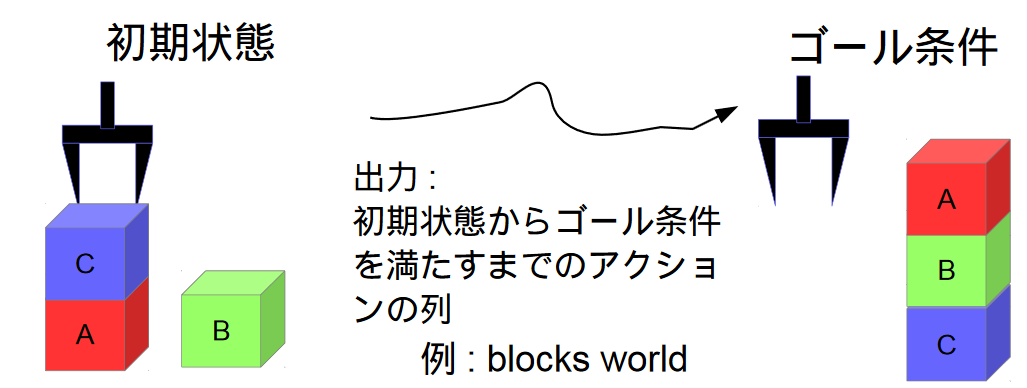
\includegraphics[width=0.8\linewidth]{./figures/blocks-image.png}
\caption{Blocks worldドメイン}
\label{fig:sliding-token}
\end{figure}

\begin{figure}
%\begin{adjustbox}{width=\textwidth,keepaspectratio}
\lstset{language=pddl,basicstyle=\ttfamily\footnotesize,breaklines=true}
\begin{lstlisting}
;;;;;;;;;;;;;;;;;;;;;;;;;;;;;;;;;;;;;;;;
;;; 4 Op-blocks world
;;;;;;;;;;;;;;;;;;;;;;;;;;;;;;;;;;;;;;;;
(define (domain BLOCKS)
  (:requirements :strips)
  (:predicates (on ?x ?y)
	       (ontable ?x)
	       (clear ?x)
	       (handempty)
	       (holding ?x)
	       )

  (:action pick-up
	     :parameters (?x)
	     :precondition (and (clear ?x) (ontable ?x) (handempty))
	     :effect
	     (and (not (ontable ?x))
		   (not (clear ?x))
		   (not (handempty))
		   (holding ?x)))

  (:action put-down
	     :parameters (?x)
	     :precondition (holding ?x)
	     :effect
	     (and (not (holding ?x))
		   (clear ?x)
		   (handempty)
		   (ontable ?x)))
  (:action stack
	     :parameters (?x ?y)
	     :precondition (and (holding ?x) (clear ?y))
	     :effect
	     (and (not (holding ?x))
		   (not (clear ?y))
		   (clear ?x)
		   (handempty)
		   (on ?x ?y)))
  (:action unstack
	     :parameters (?x ?y)
	     :precondition (and (on ?x ?y) (clear ?x) (handempty))
	     :effect
	     (and (holding ?x)
		   (clear ?y)
		   (not (clear ?x))
		   (not (handempty))
		   (not (on ?x ?y)))))
\end{lstlisting}
%\end{adjustbox}
\caption{blocks-worldのdomainファイル}
\label{fig:pddl-domain}
\end{figure}

\begin{figure}
%\begin{adjustbox}{width=\textwidth,keepaspectratio}
\lstset{language=pddl,basicstyle=\ttfamily\footnotesize,breaklines=true}
\begin{lstlisting}
(define (problem BLOCKS-3)
(:domain BLOCKS)
(:objects A B C)
(:INIT (CLEAR C) (CLEAR B) (ONTABLE C) (ONTABLE B)
 (ON C A) (HANDEMPTY))
(:goal (AND (ON A B) (ON B C)))
)

\end{lstlisting}
%\end{adjustbox}
\caption{blocks-worldのinstanceファイル}
\label{fig:pddl-instance}
\end{figure}

\section{古典的プランニング問題の例}
\label{sec:classical-planning-example}

プランニングは様々な問題解決に役立てることができる。
ここでは簡単にプランニングによってどのような問題がモデルできるかを紹介する。

\begin{enumerate}
\item エアポート (airport)
空港の地上の交通管理を行う問題である。
飛行機の離着陸の時間が与えられるのに対し、安全かつ飛行機の飛行時間を最小化する交通を求める問題である。

\item サテライト (sattellite)
人工衛星は与えられた現象を撮影し、地球にデータを送らなければならない。
このドメインはNASAの人工衛星の実際の応用から考案されたものである。

\item ローバー (rovers)
ローバーとは惑星探査ロボットのことである。
この問題は惑星探査ロボットのグループを使って惑星を探索する計画を作る問題である。
ロボットらは興味深い地形などの写真を取るなどの作業を実行する必要がある。
このドメインもNASAの応用をもとにしたものである。

\item パイプスワールド (pipesworld)
複数の原油の油田から複数の目的地にパイプを通して送りたい。
各目的地に定められた量を送るように調整することが目的である。
パイプのネットワークはグラフとしてモデルされており、また同時に原油を通せないパイプの組が存在する。

\item セルアセンブリ (cell assembly)
セルアセンブリは狭いセルの中で働き手が複雑な製品を作成する工場システムである。
大規模な製造ラインと比較して、
セルアセンブリは主に中程度の数(100個程度など)の製品を作るために使われる。
製品の開発や受注生産などに対応して、今生産しなければならない製品を手早く作成するためのセルの行動プランを考えることが問題の目的である。
\cite{asai2014fully}

\item ゲノムリアレンジメント (Genome rearrangement)
ゲノムリアレンジメントは多重整列問題の一つである。
ゲノム間の編集距離とは類似性を測るための指標として使われ、生物の進化の歴史をたどるために使われる。編集距離はあるゲノムから操作を繰り返してもう一方のゲノムに変換するためのコストの総和として定義される。
プランニングモデルを用いることでより様々な操作を定義することができる。例えば遺伝子の位置に入れ替えなど、\ref{sec:msa}節で説明したように単純にグリッド経路探索に落とし込むことのできない複雑な操作を考えることができる。
\cite{erdem2005genome}

\item トラック (trucks)
ロジスティクスと呼ばれる問題の一種である。
トラックを運転してすべての荷物をそれぞれ定められた運び先に届ける問題である。
ただしトラックが運べる荷物の総量は有限であるため、それを考慮して経路を考えなければならない。加えて、届けるまでの期限が存在する荷物が存在する。

\end{enumerate}

これらの問題はすべて問題に特化した特別なアルゴリズムをそれぞれの問題に対して開発することもできる。多くの場合、特化アルゴリズムの方が汎用プランナーよりも高速である。プランナーの利点は問題に特化した実装をしなくてもPDDLを書くだけで問題を解くことが出来るという点にある。

\section{ヒューリスティック関数の自動生成}
\label{sec:automated-heuristic}

PDDLにはヒューリスティック関数は何を使えばよいかなどの情報は書かれていない。
よって、PDDLを入力とする状態空間問題を解く場合、エージェントはヒューリスティック関数を自動生成しなければならない。
PDDLからヒューリスティック関数を自動生成する手法はプランニング研究の最も重要な研究課題の一つである。

ヒューリスティックの生成方法の一つの指針としては\ref{sec:heuristic-example}節で言及した緩和問題によるヒューリスティックが分かりやすい。
すなわち、元の問題$P$よりも簡単な問題$P'$を生成し、$P$の状態$s$から$P'$の状態$s'$へのふさわしい関数を定義する。そして$h(s)$の値を$P'$における$s'$を初期状態とするゴールへの最適解にする。
このようにしてヒューリスティック関数は自動生成することができる。

各アルゴリズムの実装はfast-downward \footnote{\url{http://www.fast-downward.org}}を参照されたい。

\subsection{ゴールカウントヒューリスティック (Goal Count Heuristic)}

多くの問題ではゴールはいくつかの条件を満たした状態の集合として与えられる。
ゴールカウントヒューリスティックは満たしていないゴール条件の数をヒューリスティック値とする関数である。
例えばスライディングタイルのゴール条件は全てのタイルが所定の位置にあることである。
なので所定の位置にないタイルの数を$h$値とすることが出来る。

ゴールカウントヒューリスティックは許容的であるとは限らない。コスト1のアクションが2つのゴールを同時に満たすかもしれないからだ。1つのアクションで同時に満たせるゴールが1つ以下である場合、そしてその時のみ、許容的である。

\subsection{適用条件緩和 (Precondition Relaxation)}

\define{適用条件緩和}{precondition relaxation}{てきようじょうけんかんわ}はアクションの適用条件を無視し、すべてのアクションをすべての状態で適用できる緩和問題を解くヒューリスティックである。すべてのアクションが適用できるようになるので、グラフのエッジの数が増えることになる。このとき、すべてのゴール条件の命題は1ステップで満たすことができる。適用条件緩和はゴールカウントヒューリスティックに近いが、少しだけ適用条件緩和の方が正確である。なぜなら適用条件緩和の場合、1. 複数のゴールを同時に満たすアクションがある場合、そのアクションを1ステップで実行することができ、2. アクションを適用することによって一旦満たされた命題が削除されることがあるからである。適用条件緩和された問題は元の問題と比べて非常に簡単になっているが、まだまだ難しい。なので更に緩和し、一度満たされた命題が削除されないとすることが多い。
こうすると緩和問題は、追加効果$add(a)$の和集合がゴール条件を全て満たす$Goal \subseteq \bigcup_{a \in A'} add(s)$ような最小のアクション集合$A'$を求める問題になる。これはまさしく\define{集合被覆問題}{set cover}{しゅうごうひふくもんだい}である \cite{karp1972reducibility}。
集合被覆問題でもまだNP困難問題であるがシンプルな貪欲で$\log n$の近似アルゴリズムになる\cite{chvatal1979greedy}。
ただし近似アルゴリズムを使う場合、許容的なヒューリスティックではなくなってしまう。


\subsection{削除緩和 (Delete Relaxation)}

\define{削除緩和}{delete relaxation}{さくじょかんわ}はアクションの削除効果を無視する緩和問題を用いたヒューリスティックである \cite{hoffmann:01a}。この緩和問題では各アクション$a \in A$の代わりに$a^+$を用いる。$a^+$は$a^+$と同じ適用条件、追加効果を持っているが削除効果が空集合である ($del(a^+) = \emptyset$)。この緩和問題における最適解のコストをヒューリスティック関数$h^+$として用いる。
緩和問題では削除効果がないので状態に含まれる命題変数は単調増加していく。そのため元の問題よりも簡単になるが、これでもまだNP困難である \cite{bylander:94}。
そのため$h^+$を非許容的に見積もるヒューリスティック、例えばadditive heuristic \cite{bonet:01a}、FF heuristic \cite{hoffmann:01a}、pairwise max heuristic \cite{mirkis2007cost}、set-additive heuristic \cite{keyder2009trees}などがつかわれる。これらを用いた場合得られるヒューリスティックは非許容的になる。

$h^+$を許容的に見積もるヒューリスティックとしてはmax heuristic $h^{max}$がある \cite{bonet:01a}。$h^{max}$はゴール条件の各命題$t \in Goal$に対してその命題一つのみをゴール条件と更に緩和した問題 ($del(a^{max}) = \emptyset, Goal^{max} = t$)を解く。このコストを$c(t)$として、$h^{max}$はその最大値である ($h^{max} = \max_{t \in Goal} c(t)$)。
$h^{max}$は許容的であるが、非許容的なヒューリスティックよりも探索の効率が悪いこと多いことが実験的に示されている。
ちなみにadditive heuristicは最大値の代わりに$c(t)$の総和を取るものである。非許容的である代わりに$h^{max}$よりも性能が良いことが多い。

\subsection{最長経路 (Critical Path)}

\define{最長経路ヒューリスティック}{critical path heuristic} \cite{haslum:00}は命題の集合を全て満たすための最小コスト$c(X)$を$X$の大きさ$m$以下の部分集合$K \subseteq X$の最大値で近似する ($c^m(X) = \max_{X' \subseteq X, |X'| \leq m} c^m(X')$)というアイディアに基づいたヒューリスティックである。この近似は下界になるので許容的なヒューリスティックが得られる。max heuristicは最長経路ヒューリスティックのうち$m=1$の場合である ($h^{max} = h^1$)。$h^m \geq h^{m-1}$なので$m$が大きいほど正確な見積もりが出来るが、同時に計算コストが$m$に対して指数的に伸びるトレードオフがある。

元々GraphPlanと呼ばれる並行プランナーで使われたアイディアに基づいている \cite{blum:97}。

\subsection{抽象化 (abstraction)}

\define{抽象化}{abstraction}{ちゅうしょうか}ヒューリスティックは状態$s$を抽象状態$\alpha(s)$への写像を用いたヒューリスティックである。
ヒューリスティック値$h^\alpha(s)$は抽象化された状態空間$S^\alpha = \{\alpha(s) | s \in S\}$でのゴールへの距離である。
抽象化は元の問題よりも簡単になるので許容的なヒューリスティックが得られる。
ヒューリスティックの性能は$\alpha$の選択による。
$\alpha$の選択方法としてはパターンデータベースヒューリスティック \cite{culberson1998pattern,edelkamp2001planning,holte:04,katz2008structural}、merge-and-shrink \cite{helmert2007flexible,helmert2014merge}などがある。


\subsection{ランドマーク (landmark)}

プランニング問題の\define{ランドマーク}{landmark}{ランドマーク}とは、全ての解の中で一度でも真になることがある命題である \cite{porteous2001extraction}。
初期状態とゴール条件に含まれる命題はランドマークである。
ランドマークの直感的な理解としては、問題を解くために通過する必要がある中間目標地点である。

\define{ランドマークカウント}{landmark count}{ランドマークカウント}ヒューリスティックはこれから通過しなければならないランドマークの数をヒューリスティック値とする。
ランドマークを全て正しく発見する問題はPSPACE困難なので近似をする必要がある。
近似の方法によって非許容的なヒューリスティック (e.g. LAMA) \cite{richter2008landmarks}を得る手法と許容的なヒューリスティックを得る手法がある \cite{karpas2009cost}。

\define{ランドマークカット}{Landmark cut}{ランドマークカット}はランドマークカウントを一般化したヒューリスティックである \cite{helmert:09}。「全ての可能な解で真になる命題」はいくつかは発見できるが、十分な数を発見するのはかなり難しい。なのでランドマークカットはその代わりに「全ての可能な解で少なくとも一つが真になる命題の集合」を使う。このような命題の集合はjustification graphと呼ばれるランドマーク発見のためのグラフのカットに相当するため、ランドマークカットと呼ばれる。


\section{関連文献}

\TODO{}


% -*- coding: utf-8 -*-

\begin{comment}

\chapter{探索問題の派生}
\label{ch:search-problem-variants}

この章では\ref{ch:state-space-problem}章で定式化した状態空間問題と少し定式化の異なる問題を扱う。
ブラックボックスプランニングは状態空間問題の一つであるが、今まで扱った問題と異なり、ドメインモデルがブラックボックスで与えられるという違いがある(\ref{sec:black-box-planning}章)。よってヒューリスティック関数を生成することが出来ず、情報なし探索が必要となる。



\section{ブラックボックスプランニング (Blackbox Planning)}
\label{sec:black-box-planning}

プランナーはPDDLを用いることでドメインの知識を吸い出し、それを利用して探索を効率化する。しかしながら、完全なモデルを得るのが難しい問題の場合、PDDLのような記述を得ることが出来ない。
例えばビデオゲームのような環境では、ゲームをクラックしない限り、完全なモデルを得ることは出来ない。
このような中身を見ることの出来ない環境でのプランニング問題をブラックボックスプランニング問題と呼ぶ。

ブラックボックスプランニングはAtari 2600や\cite{lipovetzky2015a}や、General Video Game Playing \cite{geffner2015}などのビデオゲームなどの環境に応用されている。

ブラックボックスプランニング問題は状態空間問題である。状態$s$は有限長の配列$V$で表せられ、$v \in V$の値域は$D(v)$とする。ただし、$V$の各変数がどのような意味を持つのかは未知である。
Expand関数、Goal関数はブラックボックスとして与えられる。また、ある状態に対して$A$のうち実行可能なアクションの集合が既知とは限らない\footnote{厳密にブラックボックスである場合は既知とするべきではないが、多くの研究ではオラクルによって実行可能なアクションが知らされるというモデルを用いている。}。

このようなドメインではドメインの知識を得ることが出来ないので、\ref{ch:heuristic-search}章で解説したようなヒューリスティック関数を用いることは出来ない。

幅優先探索などによってBrute-forceに探索しつくす方法を取ることも出来るが問題のサイズが大きい場合に解くことが出来ない\cite{Bellemare2013}。
Iterative Width探索 (IW search)\cite{lipovetzky2015a}は幅優先探索に新奇性による枝刈りを加えた手法である\footnote{Iterative Width探索はドメインモデルのある場合でも有用であることが知られている\cite{lipovetzkyg12}。}。IW(1)は新しく生成された状態は新しいatomを真にしない場合、枝刈りされる。

\subsection{新奇性に基づく枝刈り}
\label{sec:novelty-based-pruning}
inadmissible pruning
 Novelty-based pruning
 Iterative Width search

\subsection{ビデオゲームAI: Atari 2600} 
\label{sec:video-game}

\section{パターンマイニング}


\section{二人プレイヤーゲーム}
\label{sec:two-player-game}
and or tree
Alpha beta pruning

\subsection{αβ木}
\label{sec:alpha-beta-tree}

\subsection{Monte Carlo Tree Search}
\label{sec:monte-carlo-tree-search}


\section{オンラインプランニング}
\label{sec:online-planning}



% TODO: こういうチャプターがあるとキャッチーだね
\chapter{機械学習と探索・プランニング (Machine Learning, Search, and Planning)}
\label{ch:machine-learning}
A review of ML for AP \cite{jimenez2012review}


\section{機械学習による探索の効率化}
\label{sec:ml-for-search}
YJ DASP

\section{ドメインモデルの生成}
\label{sec:domain-acquisition}

本書を通して扱ってきた状態空間問題の大きな問題点は、問題モデルをどのように獲得するか、である。
\ref{sec:coverage}章で述べたように、本書はこれまで正しいモデルが与えられていることが前提として話を進めてきた。

%では、正しいモデルはどのようにして得るのか?
多くのアプリケーションではドメインモデル(e.g. PDDL)は人間のエキスパートが手でコーディングする。
しかしながら、この方法だと人間のエキスパートがあらかじめ想定した環境にしか適用できない。ダイナミックな環境で活躍できるようなエージェントを実装するためには、エージェントが何らかの方法でドメインモデルを生成する方法が必要である。

LOCMはプランからアクションスキームを生成する。
LOCM staticなconstraintも見つける。

階層的プランニング
オプション
Kaelbling
Konidaris et al.

\section{探索と機械学習}
\label{sec:search-and-ml}
R. Sutton
David Silver RL and simulation-based search

\subsection{Alpha Go}
\label{sec:alpha-go}

\section{参考文献}
Predictron
DL for Reward design in MCTS
Juhn, Satinder, et al.
\end{comment}

\begin{comment}
\begin{appendices}
\chapter{関連和書}

本書で扱った内容に関連する和書はいくつかある。

まず、ヒューリスティック探索は人工知能の一分野であり、人工知能の一部を実装する手法として研究されている。人工知能の金字塔であるRussel\& Norvigによる教科書は和訳も存在する\cite{russell2016artificial}。人工知能研究について興味がある読者はこれをお勧めする。

グラフ探索アルゴリズムの数学的背景は組合せ問題である。
組合せ問題についてはDonald KnuthによるThe Art of Computer Programming Volume 4A Combinatorial Algorithmsが網羅的である\cite{knuth2011art}。



\end{appendices}
\end{comment}



\bibliographystyle{spmpsci}

\bibliography{ref-jf17}

\printindex

\end{document}

